\documentclass[12pt, a4paper]{report}
\usepackage{german, isolatin1, palatino}
\usepackage[dvips]{graphicx}
\usepackage{epsfig}
\usepackage{hyperref}
\usepackage{amsmath}
\bibliographystyle{alphadin}
\author{Christian R�diger\\Christoph Reichenbach \\Markus Weimer 946371\\}

\title{\textbf{Technische Universit�t Darmstadt}\\Fachbereich Informatik\\Prof. Dr.-Ing. S. A. Huss. \vfill Entwicklung eines Mechatronik-Frameworks f�r das Projekt L�ufer \vfill }

\pagestyle{headings}
\sloppy 

\begin{document}
\maketitle

\newpage

\noindent
Verantwortlichkeit der Autoren f�r die Einzelnen Kapitel:
\begin{description}
\item[Markus Weimer] Kapitel
  \ref{laeufer_kapitel},\ref{aufgabe_kapitel}, \ref{mw_kapitel} und
  \ref{fazit_kapitel}
\item[Christoph Reichenbach] Kapitel \ref{jameson_kapitel}
\item[Christian R�diger] Kapitel \ref{cr_kapitel}
\end{description}

\vfill

\noindent
Die vorliegende Arbeit wurde im Rahmen des Projektes L�ufer erstellt.
Weitergehende Informationen zum Projekt finden sich auf dessen
Homepage:\\
http://www.projekt-laeufer.de

\newpage

\section*{Zusicherung}

Ich versichere, meine oben genannten Anteile an dieser Arbeit ohne
unzul�ssige fremde Hilfe und nur unter Verwendung der in der Arbeit
angegebenen Literatur und Hilfsmittel angefertigt zu haben.

\vspace{1cm}

\noindent
Darmstadt, den \today \hfill Markus Weimer 

\vfill

\noindent
Ich versichere, meine oben genannten Anteile an dieser Arbeit ohne
unzul�ssige fremde Hilfe und nur unter Verwendung der in der Arbeit
angegebenen Literatur und Hilfsmittel angefertigt zu haben.

\vspace{1cm}

\noindent
Darmstadt, den \today \hfill Christian R�diger

\vfill

\noindent
Ich versichere, meine oben genannten Anteile an dieser Arbeit ohne
unzul�ssige fremde Hilfe und nur unter Verwendung der in der Arbeit
angegebenen Literatur und Hilfsmittel angefertigt zu haben.

\vspace{1cm}

\noindent
Darmstadt, den \today \hfill Christoph Reichenbach


\begin{abstract}
  
  Im Rahmen des Projektes L�ufer wurde mit dieser Arbeit ein
  mechatronisches System f�r den L�ufer entwickelt. Dieses System
  schliesst drei Komponenten ein: Das Fahrerinformationssystem, eine
  Platine samt Software f�r die Entwicklung mechatronischer Systeme
  sowie eine auf CANBus basierende Kommunikationsstruktur.

  
  Die vorliegende Arbeit beschreibt die dabei getroffenen Design- und
  Produktentscheidungen vor dem Projektkontext. Im ersten Kapitel soll
  zu diesem Zweck zun�chst ein �berblick �ber das Projekt L�ufer
  gegeben werden. Darauf folgt im zweiten Kapitel eine sich aus dem
  Projekt ergebende Anforderungsdarstellund an die Mechatronik. Diese
  beiden Kapitel wurden in enger Zusammenarbeit mit den Projektleitern
  des L�ufers erstellt.
  
  Die folgenden drei Kapitel beschreiben die drei Komponenten des
  mechatronischen Systems. Dabei wird von der Anwenderschnittstelle
  �ber die Kommunikation der Ger�te bis zu den Ger�ten selbst
  vorgegangen.
  
  Im letzten Kapitel wird dann eine kurze Zusammenfassung und ein
  Ausblick gegeben.

\end{abstract}


% Inhaltsverzeichnis
\tableofcontents

% Abbildungsverzeichnis
\listoffigures

% Tabellenverzeichnis
\listoftables


\chapter{Das Projekt L�ufer}\label{laeufer_kapitel}
von: Markus Weimer
%\section{Das Projekt L�ufer}

Bei diesem Fahrzeug handelt es sich um ein von seinen Entwicklern
,,L�ufer'' getauftes Tandem, das sich durch die Vielzahl an
technischen Neuerungen auszeichnet, deren Entwicklung sich zwei Zielen
unterordnet: Reisetauglichkeit und Fahrspa�.

% Projekt
Entwickelt wird das Fahrzeug von Studenten der TU Darmstadt, TU
M�nchen sowie der FH Darmstadt in einem sehr interdisziplin�ren Team.
Beteiligt sind neben Maschinenbauern verschiedener Spezialisierungen
auch (Wirtschafts-)Informatiker, Textil- und Industrie-Designer.  Ziel
des Projektes ist die Entwicklung eines muskelgetriebenen
\emph{Reise}fahrzeugs f�r zwei Personen.  Der Schwerpunkt liegt hier
auf der Reisetauglichkeit, und nicht auf Dingen wie der theoretisch
erreichbaren Maximalgeschwindigkeit.  Neben der technischen
Herausforderung sind das Lernen in anderen Strukturen sowie die
intensive Zusammenarbeit mit Partnern aus Industrie und Forschung
Triebfedern f�r das Projekt.

% Technik 
Ein wichtiger Schritt, die Ziele Fahrspa� und Reisetauglichkeit zu
erreichen, ist die Gewichtsreduktion. So ist der L�ufer komplett aus
Aluminium und Kohlefaser gefertigt, was sein Gesamtgewicht auf ca.
$50kg$ reduziert.  Der L�ufer verf�gt im Gegensatz zu vielen anderen
muskelgetriebenen Fahrzeugen �ber eine Verkleidung. Diese dient zum
einen der Verbesserung der Aerodynamik, zum anderen aber auch als
Regenschutz.  Dies zusammen mit dem Antriebsstrang, auf den weiter
unten eingegangen werden soll, erm�glicht es zwei normal trainierten
Menschen mit dem Fahrzeug eine Durchschnittsgeschwindigkeit von ca.
$40km/h$ zu erreichen.  Dieser errechnete Wert bezieht sich allerdings
nicht etwa auf eine besonders ebene Route, sondern auf eine Strecke im
Odenwald rund um Darmstadt, also im Mittelgebirge.


% �berleitung zu Christian
Insbesondere im Bereich der Mechatronik, also der Verbindung von
Mechanik mit moderner Informationstechnologie, geht der L�ufer nicht
nur f�r Fahrrad-Verh�ltnisse neue Wege.



%%% Local Variables:
%%% mode: latex 
%%% TeX-master: "master"
%%% End:

\chapter{Aufgabenstellung}\label{aufgabe_kapitel}
von: Markus Weimer
\section{Anforderungen an die Mechatronik im L�ufer}

\cite{artikel}
\begin{description}
\item [Design]
\item [Erweiterbarkeit]
\item [Handhabbarkeit durch Ingenieure]
\item [Niedriger Stromverbrauch]
\item [Sicherheit]
\item [Fehlertoleranz]
\item [Sponsor-Barkeit]
\item [Verf�gbarkeit]
\item [Zeitlicher Rahmen des Projektes]
\end{description}


% Markus' Kapitel
\chapter{Fahrerinterface}\label{mw_kapitel}
von: Markus Weimer
\section{Aufgabenstellung}

Abbildung \ref{mw_seite} zeigt eine Seitenansicht des L�ufers.  Dabei
wurden die derzeit geplanten mechatronischen Komponenten markiert.\\
Die einzelnen Komponenten sind:

\begin{figure}
  \center
  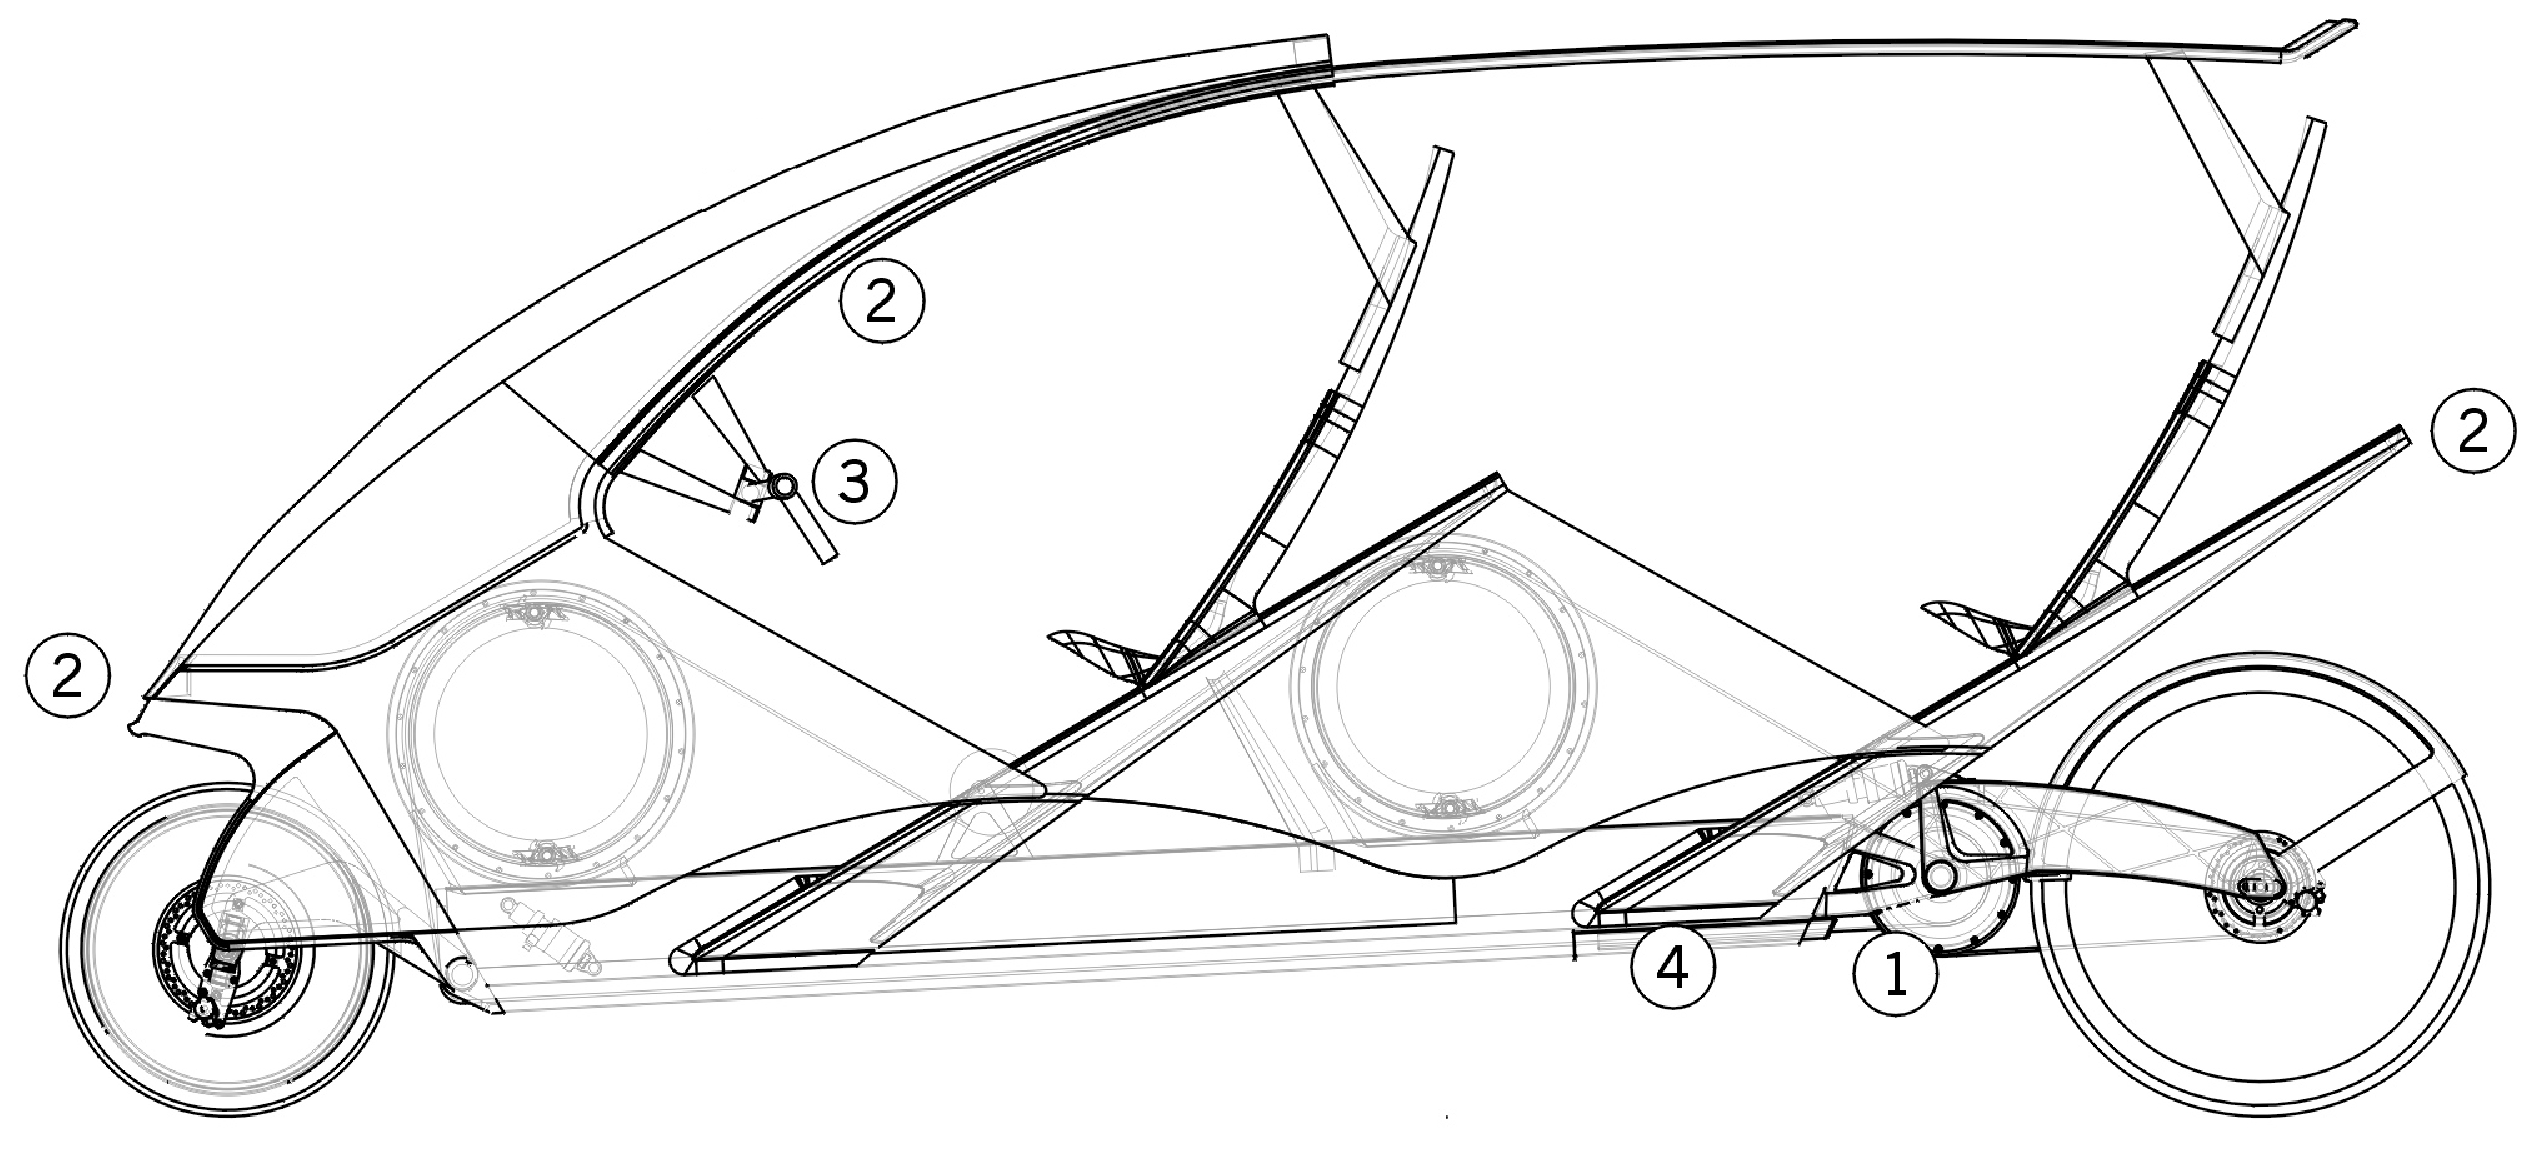
\includegraphics[width=13.5cm]{mw/bilder/seitenansicht.eps}
  \caption{Seitenansicht des L�ufers mit Markierungen der
    Mechatronischen Komponenten}
  \label{mw_seite}
\end{figure}

\begin{enumerate}
\item
  Antriebsstrang
\item
  Beleuchtungssystem 
\item
  Fahrerinformations-System
\item
  St�nder
\end{enumerate}

F�r die Zukunft sind weitere Komponenten m�glich und auch eingeplant.
Konkret angedacht wurde z.B. eine Anbindung eines GPS\footnote{Global
Positioning System}-Systems �ber den CAN\footnote{Controller Area
Network, vgl. Kapitel \ref{jameson_kapitel}}-Bus.  Die mechatronischen
Komponenten des L�ufers verf�gen �ber etliche Parameter, die der
Fahrer beeinflussen m�chte.  Als Beispiel sei hier der Antriebsstrang
genannt.  Es soll dem Fahrer z.B. erm�glicht werden, bei vollen
Batterien und kurzer Strecke alleine elektrisch zu fahren, und die
Pedale ohne Widerstand zu benutzen.

Au�erdem gibt es Informationen �ber den aktuellen Zustand des
Fahrzeuges, die an den Fahrer weitergeleitet werden m�ssen.  Dies sind
zum einen Daten, wie man Sie auch vom normalen PKW kennt, wie z.B. die
aktuelle Geschwindigkeit, zum anderen kommen beim L�ufer spezielle
Informationen aus dem Antriebsstrang hinzu: Wie schnell kann man bei der
aktuell in den Pedalen abgegebenen Energie fahren? Oder, wie voll sind
die Batterien?  Die beschriebenen Informationen m�ssen dem Fahrer in
einer Art und Weise zur Verf�gung gestellt werden k�nnen, die der
Fahrsituation angemessen ist.

Zus�tzlich ergaben Gespr�che mit den Entwicklern mechatronischer
Komponenten, da� aufwendige Berechnungen, die sich aus den W�nschen
des Fahrers ergeben, in einer relativ komfortablen Hochsprache wie
C/C++ programmierbar sein sollten, anstatt vergleichsweise umst�ndlich
in Assembler auf den Embedded Platinen.

Es ergeben sich somit die folgenden Anforderungen an das
Fahrerinformationssystem des L�ufers:

\begin{description}
\item[Gen�gend Rechenleistung:] Die geforderten Berechnungen sollen
  komfortabel in Hochsprachen durchgef�hrt werden k�nnen.
\item[Display:] Die Informationen f�r den Fahrer m�ssen dargestellt
  werden.  Aufgabe des Displays ist es, das Armaturenbrett eines PKW
  zu ersetzen.
\item[Interaktion:] Um die teilweise sehr umfassenden
  Einstellungsm�glichkeiten des Fahrzeugs ausnutzen zu k�nnen.
\end{description}

Die beschriebenen Aufgaben lassen sich in hervorragender Weise von
aktuellen Taschencomputern, sogenannten PDAs\footnote{PDA: Personal
Digital Assistent, zu Deutsch etwa: Pers�nlicher Digitaler Assistent.}
erf�llen. Exemplare der Ger�tekategorie PDA, insbesondere die neuerer
Bauart, verf�gen �ber gen�gend Rechenleistung, um die Aufgaben
innerhalb des L�ufers bew�ltigen zu k�nnen.  Zus�tzlich sind sind die
mobilen Kleicnrechner sehr stark auf den sorgsamen Umgang mit Energie
optimiert, was in einem Fahrzeug, da� seine Energie ausschlie�lich aus
der Muskelkraft seiner Fahrer bezieht, nat�rlich von besonderem
Interesse ist.  Au�erdem sind sie in gro�en St�ckzahlen kommerziell
verf�gbar, was den Preis f�r den einzelnen PDA stetig sinken l��t.

Aufgabe im Bereich des Fahrerinformationssystems ist es also
einerseits, einen geeigneten PDA auszuw�hlen und den gew�hlten
andererseits durch das Erstellen zus�tzlicher Software f�r das Projekt
nutzbar zu machen.

Die zu erstellende Software ist vor allem ein Kommunikationssystem
zwischen PDA und den im Fahrzeug verteilten Komponenten.  Dies ist
n�tig, da im PDA-Bereich zwar die aus dem PC-Markt bekannten
Schnittstellen und Kommunikationsprotokolle zur Verf�gung
stehen\footnote{Beispiele hierf�r sind die serielle Schnittstelle, die
Infrarottechnik IrDA sowie USB}. Im Bereich der mechatronischen
Systeme stehen die aus der PC-Technik stammenden Schnittstellen jedoch
im Allgemeinen nicht zur Verf�gung.  Vielmehr dominieren Protokolle
wie CAN und SPI\footnote{siehe Kapitel \ref{cr_kapitel}}.

F�r den Entwicker einer mechatronischen Komponente f�r den L�ufer mu�
die Kommunikation m�glichst einfach zu handhaben sein.  Eine solche
Forderung ergibt sich aus den �berlegungen in Kapitel
\ref{mw_problem}. Die entwickelte Software mu� diesem Umstand Rechnung
tragen, indem sie dem Entwickler eine m�glichst einfache und intuitive
Programmierschnittstelle zur Verf�gung stellt.

Neben den bisher erl�uterten Anforderungen der Entwickler
mechatronischer Komponenten soll aber gerade bei der Auswahl des PDAs
der sp�tere Nutzer des L�ufers und seine W�nsche Ber�cksichtigung
finden. Der potentielle L�uferfahrer bzw. die potentielle Fahrerin
w�nscht sich von einem solchen Ger�t einen Mehrfachnutzen.  Es soll
also sowohl als ,,Bordcomputer'' des L�ufers fungieren k�nnen, als
auch ein vollwertiger PDA sein.

Im folgenden soll zun�chst die Entscheidung f�r einen speziellen PDA
transparent gemacht werden.  Daraufhin wird die
Kommunikations\-schnittstelle f�r die Entwickler mechatronischer
Komponenten f�r den L�ufer beschrieben.

Im Bereich der Projektarbeit ergeben sich nat�rlich auch
Anforderungen, die sich nicht direkt aus theoretischen Erw�gungen
ableiten lassen k�nnen.  Viele Anforderungen werden erst und immer
wieder im Gespr�ch mit den Projektteilnehmern aus anderen
Fachgebieten, wie z.B. dem Maschinenbau oder dem Industriedesign,
deutlich.  Ergebnisse dieser Anforderungen sind unter anderem der so
genannte DebugTreiber, auf den am Ende des aktuellen Kapitels
exemplarisch f�r die interdisziplin�re Zusammenarbeit innerhalb des
Projektes eingegangen werden soll.


\newpage
\section{Auswahl des PDA}
\subsection{Anforderungen}
Die Anforderungen an den PDA ergeben sich aus den Anforderungen an die
gesamte Mechatronik sowie an das Fahrerinformationssystem im
speziellen.  Sie lassen sich in Anforderungen an die PDA
Systemsoftware und Anforderungen an die PDA-Hardware gliedern, was im
folgenden geschehen soll.  Eine Gliederung nach Betriebssystem ist
hilfreich, da sich auch der PDA-Markt sehr gut nach der Systemsoftware
der PDAs unterteilen l��t.  Weiter unten wird dies zur Vorauswahl des
PDAs ausgenutzt.

\subsubsection{Anforderungen an die Software}
\begin{description}
\item[Multitasking:] Hierbei verstehen wir unter ,,Multitasking'' die
  F�higkeit des PDA, mehrere Programme unabh�ngig voneinander
  auszuf�hren.  Die Anforderung nach Multitasking ergibt sich
  unmittelbar aus der Forderung an die gesamte Mechatronik,
  erweiterbar zu sein.  Ein PDA ohne Multitasking w�rde allerdings bei
  jeder Erweiterung des Systems einen Eingriff in die
  sicherheitsrelevante Fahrsoftware des L�ufers erfordern, was z.B.
  beim Einf�gen eines GPS\footnote{GPS=Global Positioning System}
  basierten Navigationssystems nicht w�nschenswert ist.  Verf�gt der
  PDA hingegen �ber Multitasking, kann eine Erweiterung auch durch ein
  weiteres Programm geschehen, da� parallel zu den anderen l�uft.
  
\item[GUI-Flexibilit�t:] Das Projekt L�ufer geht in vielen Bereichen
  einen designorientierten Weg, der nicht unerheblich zu dem gro�en
  Erfolg des L�ufers in der �ffentlichkeit sowie beim Aufbau von
  Industrie-Partnerschaften beigetragen hat.  Auch im Bereich der
  graphischen Interaktion mit dem System soll ein designorientierte
  Weg m�glich sein, um den L�ufer als ,,rundes Produkt'' entwickeln zu
  k�nnen.
  
  Bei der Auswahl eines PDA samt zugeh�riger Software ist demgem��
  darauf zu achten, da� man im Bereich der Gestaltung des
  GUI\footnote{GUI=Graphical User Interface, zu Deutsch: Graphische
    Benutzer Schnittstelle} gr�sst\-m�gliche Freiheiten hat.
  
\item[Programmierung:] Die Programmierung des PDA sollte einfach sein,
  wobei mit ,,einfach'' im Kontext des L�ufers gemeint ist, da� die
  Entwicklung f�r den PDA sich m�glichst wenig von der Entwicklung f�r
  einen PC unterscheiden sollte.  Das ist sinnvoll und w�nschenswert,
  da die sp�teren Nutzer unserer Software wahrscheinlich schon �ber
  Erfahrungen in der Programmierung von PCs verf�gen und deren
  Lernaufwand ja so niedrig wie m�glich zu halten ist.
  
  Au�erdem erm�glicht eine solche Vorgehensweise idealerweise die
  Entwicklung der Software auf einem PC, um sie dann sp�ter ohne gro�e
  Umst�nde einfach auf den PDA �bertragen zu k�nnen.  Inbesondere vor
  dem Projekthintergrund und der verteilten Produktentwicklung kann
  ein so ausgelegtes Vorgehen erhebliche Kosten f�r die Beschaffung
  von PDAs f�r die einzelnen Entwicklerteams in Darmstadt und M�nchen
  einsparen.
  
\item[Dokumentation und Support:] Da die Entwicklung der Software �ber
  die vorliegende Studienarbeit hinaus von weiteren Entwicklern
  fortgesetzt werden soll, ist eine gute Dokumentation und ein
  umfassender Support der verwendeten Werkzeuge, Bibliotheken und
  Compiler mehr als w�nschenswert.
  
  Aus den selben Gr�nden ist es n�tig, auf eine m�glichst
  ,,langlebige'' Plattform zu setzen, die sich nicht innerhalb des
  Projektes st�ndig ver�ndert oder f�r deren eingesetzte Version man
  in Zukunft wom�glich keine Entwicklungstools mehr erwerben kann.
  
\end{description}


\subsubsection{Anforderungen an die Hardware}
An die Hardware eines PDA f�r den Einsatz in einem Fahrzeug stellen
sich besondere Anforderungen, die im folgenden erl�utert werden
sollen.

\begin{description}
\item[Display:] Beim Display eines PDA f�r den Einsatz im L�ufer gibt
  es zwei wesentliche Aspekte zu beachten: Zum einen sollte es sich um
  ein Farbdisplay handeln und zum anderen sollte es vor allem unter
  all den Lichtbedingungen, in denen der L�ufer unterwegs sein wird,
  gut ablesbar sein.
  
  Die Forderung nach einem Farbdisplay ergibt sich aus der
  Design-Orientierung des Projektes sowie der Anforderung nach
  GUI-Flexibilit�t.  Desweiteren spricht f�r ein Farbdisplay,da� man
  mit ihm Warnhinweise und normale Nachrichten des Systems auf dem
  Display farblich kodieren kann, wie man dies von anderen Ger�ten
  kennt.  So lassen sich durch Farbe gerade im Fahrbetrieb wichtige
  Informationen hervorheben, was z.B. beim PKW mit seinen \emph{roten}
  Warnleuchten ebenfalls geschieht.
  
  Die Anzeigeeigenschaften des Display bei sehr extremen
  Lichtverh�ltnissen sind f�r den L�ufer entscheidend.  Das Display
  mu� bei allen Fahrsituationen m�glichst gut ablesbar sein, um den
  Fahrer �ber den aktuellen Zustand seines Fahrzeuges zu informieren.
  Zu den kritischen Lichtverh�ltnissen geh�rt dabei weniger die Nacht,
  da alle modernen PDAs �ber eine leistungsf�hige Beleuchtung
  verf�gen.  Wesentlich wichtiger ist das Verhalten w�hrend der
  D�mmerung und bei starkem Sonnenschein.  Beides stellt einige
  Display-Konzepte bei heute markt�blichen PDAs vor gro�e Probleme.
  
  Als Beispiel sei hier die inverse Hintergrundbeleuchtung der PDAs
  des Herstellers Palm genannt, die zwar bei absoluter Dunkelheit
  hervorragende Dienste leistet, bei D�mmerung aber zu Unlesbarkeit
  des Displays f�hrt.
  
\item[Optik:] Ein ebenfalls nicht zu untersch�tzender, wenn auch nur
  subjektiv zu beurteilender, Bereich ist die optische Erscheinung des
  PDA.  Die Optik spielt aus technischer Sicht nat�rlich nur eine
  untergeordnete Rolle, wird jedoch im Projektkontext bedeutsam.
  Erkennen l�sst sich die Bedeutung des Designs f�r den L�ufer an dem
  Umstand, dass einige Elemente des L�ufers nur unter �sthetischen
  Gesichtspunkten zu Stande gekommen sind.  Da sich unsere Arbeit in
  das Projekt integriert, m�ssen wir dem Gesichtspunkt Optik ebenfalls
  Bedeutung zumessen.
  
  Ein objektiv nachpr�fbarer Bereich der Optik ist die Bauform.  F�r
  den Einsatz im L�ufer kommen nur sogenannte Stift-PDAs in Frage, bei
  denen das Display hochkant steht und die Eingabe �ber einen Stift
  erfolgt.  Unter den bekannten um am Markt vertretenen Bauformen l��t
  sich ein Hochkant-Design am besten in das Fahrzeug-Cockpit des
  L�ufers integrieren.
  
\item[Anschlu�m�glichkeiten:] Da das Projekt L�ufer eines mit
  ausser\-gew�hnlicher Dynamik ist, ist die Anschlussvielfalt an einem
  PDA im L�ufer ein wesentliches Argument, um sich sp�tere
  Erweiterungen nicht durch einen zu beschr�nkten PDA zu verbauen.
  
  Die Mindestanforderung im Schnittstellen-Bereich ist eine
  RS232\footnote{Im PC-Bereich auch h�ufig nur ,,serielle
    Schnittstelle'' genannt.}  Schnittstelle, da �ber die serielle
  Schnittstelle die Verbindung zu einer unserer Platinen hergestellt
  wird.  Die Platine am anderen Ende der RS232-Schinttstelle verbindet
  dann den PDA mit dem CAN-Bus. Zu Details der Kommunikation im L�ufer
  siehe Kapitel \ref{jameson_kapitel}.
\end{description}


\subsection{Auswahl der Systemsoftware}
Der PDA Markt l��t sich, wenn man die diversen geschlossenen Systeme
au�er Acht l��t, nach den Betriebssystemen PalmOS, WindowsCE und
Linux aufgliedern.  Die ebenfalls noch angebotenen PDAs der Firma
PSION finden hier keine Beachtung, da deren Vermarktung und
Weiterentwicklung mittlerweile eingestellt wurde.  Au�erdem pa�t
deren Tastatur-Orientiertes Design nicht in das Konzept des
Cockpit-Entwurfs f�r den L�ufer.

Die Einteilung nach Betriebssystem lieferte eine erste Kategorisierung
des PDA-Marktes.  Zu jedem System sind relativ viele verschiedene PDAs
am Markt, wordurch die Entscheidung f�r ein bestimmtes Betriebssystem
die erste zu treffende war.

\subsubsection{�bersicht �ber PDA-Betriebssysteme}
Im folgenden sollen die einzelnen Systeme samt ihrer f�r das Projekt
relevanten Eigenschaften vorgestellt werden, um sich f�r eins zu
entscheiden, da� die software-seitigen Voraussetzungen f�r einen
Einsatz im L�ufer mitbringt.

\begin{description}
\item[PalmOS:] Das System ,,PalmOS'' wurde von der Firma 3Com
  entwickelt und zu\-n�chst ausschlie�lich auf deren PDAs, den
  sogenannten ,,PalmPilots'' eingesetzt.  Mittlerweile hat es PalmOS
  zur Marktf�hrerschaft gebracht und ist auch auf den Ger�ten von
  Herstellern wie Sony, Handspring und anderen zu finden.
  
  Folglich ist es verst�ndlich, dass als erstes Ger�te mit dem System
  des Marktf�hrers ins Auge gefa�t wurden.  Bei den Ger�ten kann man
  aufgrund der gro�en Verbreitung mit einer guten Akzeptanz seitens
  der Nutzers des L�ufers rechnen.  Auch wird ein eventueller Kunde
  mit hoher Wahrscheinlichkeit schon �ber ein solches Ger�t verf�gen.
  
  Ein ,,Palm IIIx'' wurde dann auch Basis eines ersten Versuchs der
  Mechatronik, der im Rahmen einer Studienarbeit von J�rn
  Schlingen\-siepen\cite{Schlinge} stattfand.  Im Rahmen der Arbeit
  wurde die grund\-s�tzliche M�glichkeit der Anbindung eines solchen
  Ger�tes an den CANBus untersucht und auch best�tigt.
  
  Allerdings verf�gt PalmOS in seiner jetzigen Version nicht �ber
  Multitasking, was einen Einsatz im L�ufer nicht erm�glicht.  Die
  geforderte Erweiterbarkeit wird nicht in dem Ma�e sicherstellt, wie
  es im L�ufer erforderlich ist.
  
  Im Bereich der Graphischen Gestaltung des Fahrerinterface erwiesen
  sich die verf�gbaren Ger�te mit PalmOS als recht eingeschr�nkt, da
  sie weder �ber eine anpa�bare Bibliothek von Oberfl�chenelementen
  noch �ber gen�gend Rechenleistung verf�gen, um die GUI selbst zu
  ,,malen''.  Bei einem System wie PalmOS ist das jedoch kein
  Design-Fehler, sondern schl�gt sich z.B. in der �berwiegend
  konstanten und guten Bedienbarkeit der Software f�r die PalmOS-PDAs
  nieder.  Die an sich gute Eigenschaft wirkt aber vor dem Hintergrund
  unserer Aufgabe negativ aus.
  
  Die Programmierung eines PalmOS-PDAs erfolgt mit speziellen Tools.
  Allerdings haben sich Ger�te mit PalmOS im Laufe der Zeit so weit
  verbreitet, da� mehrere alternative Programmierumgebungen und
  Compiler zur Verf�gung stehen.  Auch hat die hohe Verbreitung zu
  einer guten und frei verf�gbaren Dokumentation der
  Programmierschnittstelle und -Praktiken f�r das Betriebssystem
  PalmOS gef�hrt.
  
\item[WindowsCE / Pocket PC:] PDAs mit dem System aus dem Hause
  Microsoft zeichnen sich durch Ihre leistungsf�hige Hardware aus.  So
  ist es bei WindowsCE-Ger�ten nicht selten, einen Prozessor mit
  deutlich mehr als 200MHz Taktfrequenz vorzufinden.
  
  Auch verf�gt Windows CE �ber Multitasking, eine permanent im
  Hintergrund laufende Fahrsoftware ist also mit dem System
  realisierbar.
  
  Die graphische Oberfl�che ist sehr an die Desktop-Versionen von
  Windows angelehnt.  Die Flexibilit�t bei der Gestaltung einer
  Oberfl�che f�r die L�ufersoftware ist auch unter Ber�cksichtigung
  der Einschr�nkung durch die Festlegung auf eine Entwicklungsumgebung
  schon alleine deshalb gro�, weil die Ger�te �ber so gro�e
  Leistungsreserven verf�gen.  Im Prinzip wird sogar eine komplett
  ,,gemalte'' Oberfl�che erm�glicht, auch wenn die dann recht viel
  Speicher verbraucht.
  
  Die Programmierung des Systems erfolgt mittels der bekannten
  Microsoft-Tools wie z.B. Visual C++, welche schon alleine aufgrund
  ihrer Verbreitung bestens dokumentiert sind.  Allerdings ist
  WindowsCE genauso wie PalmOS ein reines PDA-System, so da� die
  Entwicklung f�r diese PDAs mit den speziellen Tools erfolgen mu� und
  zum Testen der Software ein Emulator zum Einsatz kommt.
  
\item[Linux:] Linux ist im gesamten PDA und Embedded-Bereich ein
  Neuling, allerdings mit steigender Verbreitung.  Die steigende
  Verbreitung ist vor allem auf die gro�e Flexibilit�t des Systems
  zur�ckzuf�hren.
  
  Linux verf�gt nat�rlich auch auf dem PDA �ber echtes Multitasking.
  Schlie�lich kommt der selbe Kernel und die selbe Systemsoftware zum
  Einsatz wie auf den anderen Plattformen, auf denen es eine
  Implementierung des freien Betriebssystems gibt.
  
  Die Gleichheit in der Software bringt Linux auf dem PDA eine gro�e
  Flexibilit�t, da direkt die gesamte Software, die es f�r Linux gibt,
  verf�gbar ist.  Betroffen hiervon sind insbesondere die Bibliotheken
  f�r Entwickler.  So existieren z.B. mehrere GUI-Bibliotheken, die
  noch dazu auf verschiedenen Wegen mit der Hardware kommunizieren
  k�nnen.
  
  Aus der identischen Software auf PC/Workstation und PDA folgt aber
  auch, da� man Software f�r den PDA unter Ber�cksichtigung einiger
  Randbedingungen auf dem PC entwickeln und testen kann.  Dabei kann
  auf einen Emulator der PDA-Hardware verzichtet werden.  Hierdurch
  wird es erm�glicht, da� Entwickler Software auf Ihrem PC entwickeln
  und mit diesem testen, die dann sp�ter durch ein Neu�bersetzen
  \footnote{Diesen Vorgang nennt man im Allgemeinen
    ,,crosscompiling''} auf den PDA portiert werden kann.
  
  Die gro�e Flexibilit�t zieht allerdings auch einen entscheidenden
  Nachteil nach sich: Nahezu jeder Entwickler f�r Linux-basierte
  Embedded Systems arbeitet mit seinem eigenen Set an Tools,
  Bibliotheken und Compilern.  Daraus folgt, da� es keine gro�e
  Entwicklergemeinde gibt, die alle mit den selben Tools arbeiten, was
  zu einer Un�bersichtlichkeit der Dokumentation f�hrt.  Die
  Un�bersichtlichkeit wird allerdings durch die Gleichheit des
  Systems zu dem auf PCs teilweise wieder ausgeglichen.
\end{description}  


\subsubsection{Entscheidung}
Tabelle \ref{mw_pda_os_tabelle} zeigt nochmals eine �bersicht der
Systeme mit ihren individuellen Eigenschaften.

PalmOS ist wegen der fehlenden Multitasking-F�higkeit f�r unsere
Aufgabe ungeeignet.  Somit musste die Entscheidung zwischen Linux und
Windows CE getroffen werden.
  
Wir haben uns letztendlich f�r Linux entschieden, um uns die gr��te
Flexibilit�t zu sichern.  Betroffen hiervon ist nicht nur die oben
schon ausgef�hrte Auswahl an GUI-Bibliotheken, sondern auch die
M�glichkeit im Falle der Notwendigkeit selbst am Betriebssystem Hand
anlegen zu k�nnen.  Da wir ein klassisches Embedded System durch einen
handels�blichen PDA ersetzten, war zu Beginn nicht klar, welche
Probleme dabei auftreten k�nnen.  Und mit einem unab�nderlichen
Betriebssystem w�ren solche Probleme eventuell nicht l�sbar.
  
Zus�tzlich ist es mit einem Linux-PDA m�glich, Software auf PCs zu
entwickeln und zu testen, ohne da� dazu ein PDA oder gar ein Emulator
n�tig ist.

\begin{table}
  \caption{�bersicht �ber die verschiedenen PDA-Betriebssysteme}
  \label{mw_pda_os_tabelle}
  \begin{center}
    \begin{tabular}{|c|c|c|c|}
      \hline
      \emph{Anforderung} & \emph{PalmOS} & \emph{WindowsCE} & \emph{Linux} \\
      \hline
      \emph{Multitasking} &$\circ$ &$\bullet$ & $\bullet$\\
      \hline
      \emph{GUI-Flexibilit�t} &$\circ$ &+ & ++\\
      \hline
      \emph{Programmierung} &$\circ$ &+&++\\
      \hline
      \emph{Dokumentation und Support} &++ &+ &+\\
      \hline
    \end{tabular}
  \end{center}
\end{table}



\subsection{Auswahl der Hardware\label{mw_pda_uebersicht}}
Im folgenden sollen kurz die PDAs beschrieben werden, die f�r das
Projekt in Frage kamen, und die in folge dessen auch n�her gepr�ft
wurden.

Da der Markt f�r Linux-basierte PDAs sehr in Bewegung ist, kann und
soll hier keine vollst�ndige und insbesondere keine aktuelle �bersicht
gegeben werden.  Ein guter Anlaufpunkt f�r eine solche ist die
Homepage von Linuxdevices\footnote{http://www.linuxdevices.com}.



\begin{description}
\item[Agenda VR3:] Diesem PDA, der in Abbildung \ref{mw_agenda} zu
  sehen ist, geb�hrt die Ehre des ,,first-to-market''-Ger�tes im
  Bereich Linux-PDAs, da es Agenda Computing als erstes gelang, einen
  endkundentauglichen PDA mit Linux als Betriebssystem in die L�den zu
  bringen.
  \begin{figure}
    \center
    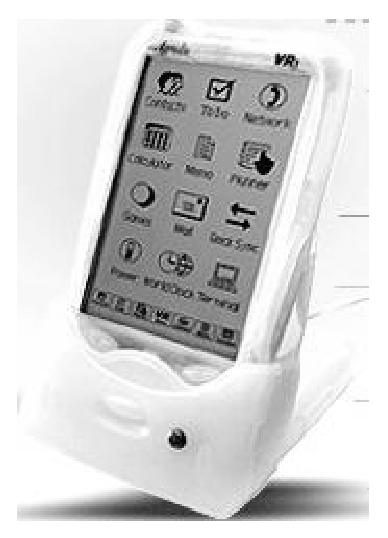
\includegraphics[width=7.0cm]{mw/bilder/agenda.eps}
    \caption{Der Agenda VR3}
    \label{mw_agenda}
  \end{figure}
  
  Leider gab es zum Zeitpunkt der Entscheidung noch keine
  Farb-Variante dieses Ger�ts. Farbe ist aber in einer
  Design-orientierten Entwicklung wie dem L�ufer ein absolutes Mu�.
  
\item[G.Mate Yopy:] Abbildung \ref{mw_yopy} zeigt den G.Mate Yopy, der
  lange Zeit als Mythos durch die diversen News-Seiten und -Foren des
  Internet geisterte. Ihm wurde am ehesten zugetraut, der erste
  brauchbare PDA mit Linux als Betriebssystem zu sein.  Die Hoffnung
  der Linux-Enthusiasten wurde nicht zuletzt durch die Pr�sentation
  des Yopy auf der CeBIT 2000 durch den damaligen G.Mate-Partner
  Samsung gen�hrt.

  \begin{figure}
    \center
    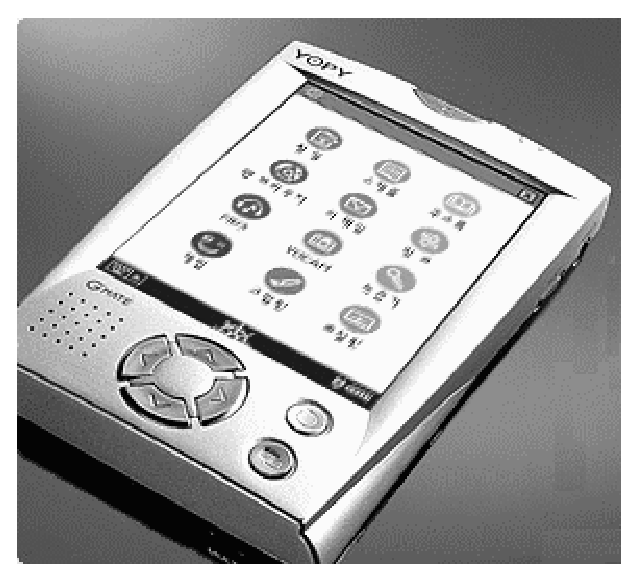
\includegraphics[width=7.0cm]{mw/bilder/yopy.eps}
    \caption{Der G.Mate Yopy}
    \label{mw_yopy}
  \end{figure}
  
  Nachdem Samsung jedoch aus dem Projekt ausgestiegen ist, ist es
  ruhig um den Yopy geworden. In Deutschland war kein solches Ger�t
  auszumachen.  Somit kam der Yopy leider nicht f�r das Projekt in
  Frage, zumal seine Zukunft nach wie vor ungekl�rt ist und somit eine
  Versorgung der Nullserie des L�ufers mit Ger�ten nicht sicher war.
  
  Auf der CeBIT 2002 wurde der Yopy wieder gezeigt, jedoch nun mit
  einem v�llig neuen mechanischen Aufbau, der an ein klappbares
  Mobiltelefon erinnert.  Eine solche Form pa�t nicht zu den Anforderungen
  an einen PDA im L�ufer, weshalb sich die Entscheidung gegen diesen
  PDA auch im Nachhinein als richtig erwiesen hat.

  
\item[VTech Helio:] Siehe Abbildung \ref{mw_helio}.  Hierbei handelt es
  sich um einen PDA der Firma VTech, der mit dem propriet�ren VT-OS
  als Betriebssystem betrieben wird.  VTech unterst�tzt allerdings
  auch die Entwicklung einer Linux-Distribution f�r den Helio.
  \begin{figure}
    \center
    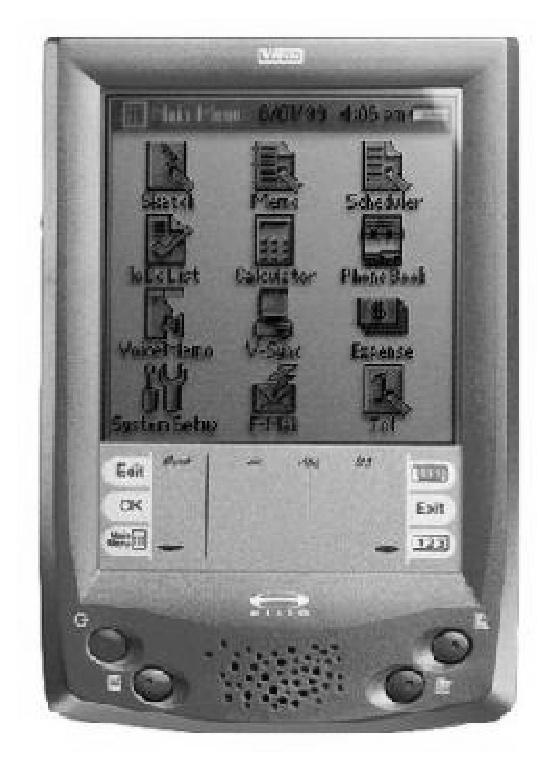
\includegraphics[width=7.0cm]{mw/bilder/helio.eps}
    \caption{Der VTech Helio}
    \label{mw_helio}
  \end{figure}
  
  Der PDA macht von seiner �u�eren Erscheinung mehr den Eindruck eines
  Spielger�tes f�r Kinder, was ja auch der Haupt-Markt des Anbieters
  VTech ist.  Der PDA verf�gt ausserdem nicht �ber ein Farb-Display,
  so da� er f�r das Projekt ebenfalls nicht in Frage kam.
  
  
\item[Casio Cassiopeia:] Die PDAs dieser Serie sind �beraus
  leistungsf�hig.  Sie verf�gen �ber einen Prozessor auf Basis der
  MIPS-Architektur bei 125MHz-150MHz, bis zu 32MB RAM und Farbdisplays
  mit einer Aufl�sung von 320x240 Pixel.  Auf der Seite der Hardware
  spricht also vieles f�r den Cassiopeia. Abbildung \ref{mw_casio}
  zeigt den Cassiopeia.
  
  \begin{figure}
    \center
    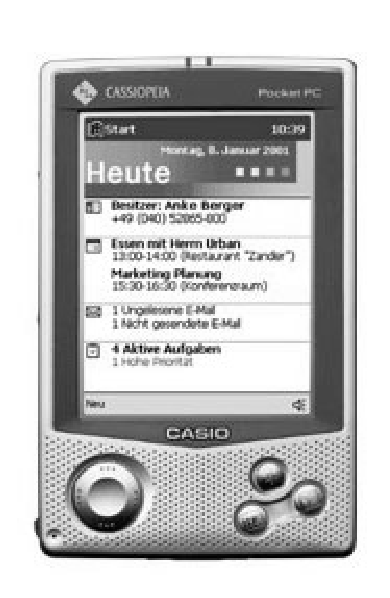
\includegraphics[width=7.0cm]{mw/bilder/casio.eps}
    \caption{Der Casio Cassiopeia}
    \label{mw_casio}
  \end{figure}
  
  Ebenfalls verf�gbar ist eine Implementierung des Linux Kernels f�r
  diese Ger�te.  Allerdings besitzen die Ger�te dieser Serie kein
  wiederbeschreibbares Flash-ROM, sondern nur ein ROM f�r das
  Betriebssystem, so da� ein Start von Linux immer �ber spezielles
  WindowsCE Programm namens ,,CyaCE'' erfolgen mu�.  Im Rahmen einer
  \emph{Produkt}entwicklung ist es jedoch nicht w�nschenswert, dass
  sich ein potentieller Nutzer zu sehr mit den technischem
  Details des Fahrzeuges auseinandersetzen mu�.
  
  Ein weiteres, nicht zu untersch�tzendes Argument gegen die Ger�te
  dieser Serie ist, da� sie von einem Asiatischen Hersteller
  vertrieben werden, und diese sich bisher als eher unwillige
  Sponsoren des Projektes erwiesen haben.
  
  
  
\item[Compaq IPAQ:] Der Compaq IPAQ (siehe auch Abbildung
  \ref{mw_ipaq_bild}) ist von der Hardware her dem Sharp-PDA sehr
  �hnlich, der einzige Unterschied liegt in der standardm��ig
  ausgelieferten Software.  Der IPAQ kommt standardm��ig mit Windows
  CE, w�hrend der Sharp mit Linux ausgestattet wird.
  \begin{figure}
    \center
    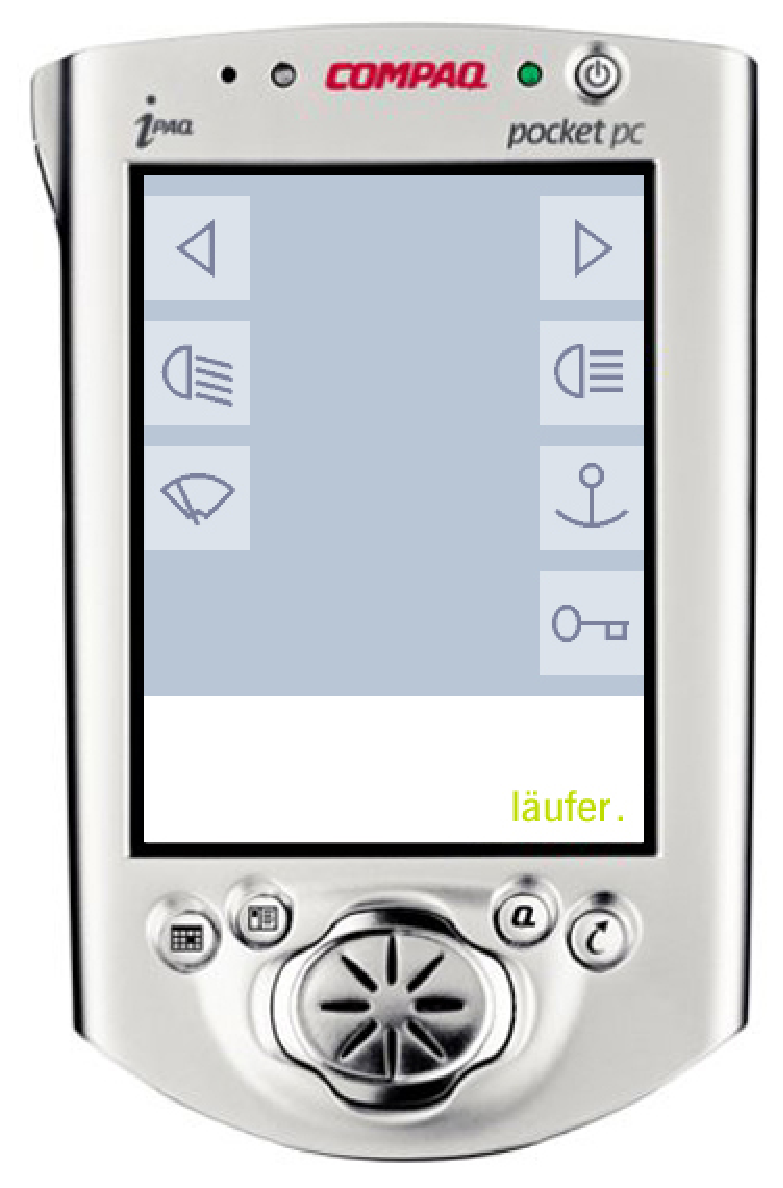
\includegraphics[width=7.0cm]{mw/bilder/Menu.eps}
    \caption{Der Compaq IPAQ mit der L�ufer-Software f�r die Cebit 2002}
    \label{mw_ipaq_bild}
  \end{figure}
  
  F�r den IPAQ existiert allerdings eine sehr weit fortgeschrittene
  Portierung des Linux Kernels und etlicher Programme, so da�
  mittlerweile sogar schon mehrere Distributionen um die Gunst des
  IPAQ-Besitzers buhlen.  Siehe dazu auch Kapitel \ref{mw_ipaq_linux}
  
  Die Hardware des IPAQ H3660 stellt wohl derzeit das technisch
  machbare im PDA-Umfeld dar. Das Ger�t bietet Leistungen, die ein
  Entwickeln auf normalen Desktop-Rechnern erm�glicht, ohne das
  Unbehagen, die Zielplattform k�nnte eine bestimmte Funktionalit�t
  aus Gr�nden der dort vorhandenen Ressourcen nicht zur Verf�gung
  stellen.
  
  Die Hardware des IPAQ im Einzelnen:
  
  \begin{description}
  \item[CPU:] StrongARM 206MHz
  \item[RAM:] 64MB
  \item[Flash:] 16MB interner Flash-Speicher
  \item[Display:] 240x320 12Bit reflektives Farbdisplay
  \item[Schnittstellen:] RS-232, USB, IRDA, Analog Sound
  \item[Erweiterungen:] Es besteht die M�glichkeit, den IPAQ um
    folgende Slots zu erweitern: CompactFlash, 1x PCMCIA oder 2x
    PCMCIA.  Hierzu wird der IPAQ in seine eigene Erweiterung, ein so
    genanntes ,,Jacket'' hineingesteckt, was Ver�nderungen im
    Formfaktor zur Folge hat. Die Jackets gibt es in Ausf�hrungen mit
    den genannten Steckplatz-Konfiguration.
  \end{description}
  
\item[Sharp Zaurus:] Dieser PDA verf�gt �ber �hnliche technische Daten
  wie der Compaq IPAQ.  Wie dieser verf�gt er �ber einen StrongARM
  206MHz Prozessor, 64MB RAM und 16MB Flash.  Auch das Display ist
  �hnlich dem des Compaq. Abbildung \ref{mw_sharp} zeigt dieses Ger�t.

  \begin{figure}
    \center
    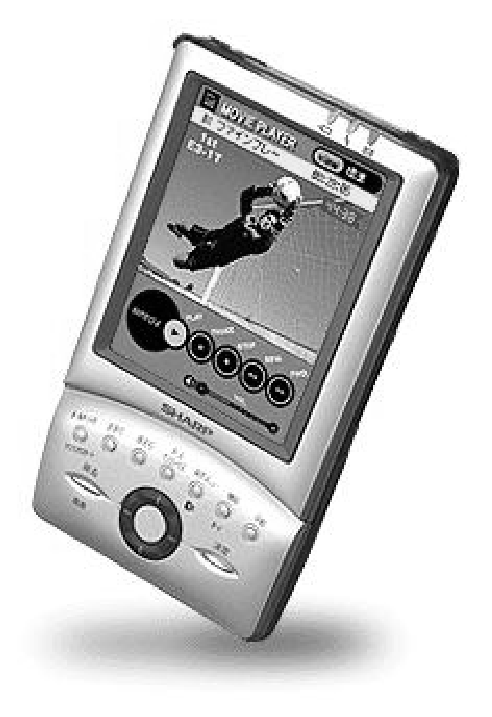
\includegraphics[width=7.0cm]{mw/bilder/sharp.eps}
    \caption{Der Sharp Zaurus}
    \label{mw_sharp}
  \end{figure}
  
  Allerdings wird der zu Beginn der vorliegenden Arbeit noch nicht mit einem
  Namen versehene PDA nicht mit Windows CE, sondern mit Linux als
  Betriebssystem ausgeliefert. Die Software entspricht weitgehend der,
  die wir auf dem IPAQ einsetzen. Es kommt also ein Linux Kernel 2.4.X
  mit QTopia als graphischer Oberfl�che zum Einsatz.
  
  Leider war das Ger�t zu Beginn unserer Arbeit noch nicht verf�gbar,
  so da� wir das von all seinen Daten her ideale Ger�t leider nicht
  verwenden konnten.  Auf der Cebit 2002 wurden erste Kontakte mit
  Sharp gekn�pft, um ein eventuelles Wechseln auf den Sarp Zaurus
  vorzubereiten.

\end{description}

\subsubsection{Entscheidung}
Tabelle \ref{mw_pda_tabelle} zeigt nochmals eine �bersicht �ber die
verschiedenen PDAs mit ihren individuellen Eigenschaften.  Die Wahl
fiel letztlich auf einen Compaq IPAQ, da das Ger�t nach den
Informationen, die zur Zeit der Entscheidung im WWW zur Verf�gung
standen, �ber die weitestgehende Unterst�tzung unter Linux verf�gt.
Ein weiteres wesentliches Argument f�r dieses Ger�t ist das reflektive
Display. Dadurch wird eine Nutzung als zentrale Anzeige in einem
Fahrzeug �berhaupt erst m�glich.  Durch das reflektive Display wird
die Anzeige des IPAQ bei st�rkerer Sonneneinstrahlung automatisch
heller, so da� im Gegensatz zu z.B. Notebooks ein Ablesen auch im
Sommer bei gro�er Helligkeit m�glich ist.

Leider war es zu Beginn der vorliegenden Arbeit nicht m�glich, den
Sharp Zaurus zu ber�cksichtigen, da er zu diesem Zeitpunkt nicht zur
Verf�gung stand.  Im weiteren Projektverlauf wird allerdings versucht,
auf den Zaurus umzusteigen, da er �ber �hnliche Leistungen wie der
IPAQ verf�gt, jedoch direkt mit Linux ausgeliefert wird.  Die
Verwendung eines Standard-PDA macht vor dem Hintergrund einer

\emph{Produkt}entwicklung nat�rlich Sinn.
\begin{table}
  \caption{�bersicht �ber die verschiedenen Linux-f�higen PDAs}
  \label{mw_pda_tabelle}
  \begin{center}
    \begin{tabular}{|c|c|c|c|c|}
      \hline
      \emph{Anforderung} & \emph{Display} & \emph{Optik} & \emph{Anschlu�m�glichkeiten} & \emph {Verf�gbarkeit}\\
      \hline
      \emph{VR3}         & -- & 0 & 0 & + \\
      \hline
      \emph{Yopy}        &  + & + & 0 & -- \\
      \hline
      \emph{Helio}       & -- & --& 0 & + \\
      \hline
      \emph{Cassiopeia}  &  + & + & + & -- \\
      \hline
      \emph{Zaurus}      & ++ & + & + & (-) \\
      \hline
      \emph{IPAQ}        & ++ & ++& + & + \\
      \hline
    \end{tabular}
  \end{center}
\end{table}


\subsection{Zusammenfassung}
Wie weiter oben beschrieben wurde die Entscheidung zugunsten von Linux
gef�llt; Linux auf dem PDA ist sehr PC-�hnlich zu programmieren und
verf�gt �ber Multitasking.  Au�erdem ist es im Bereich der GUI sehr
flexibel und es ist nicht unbedingt ein PDA n�tig, um Komponenten f�r
die L�ufer-Software zu entwickeln.

F�r den IPAQ wurde sich entschieden, weil er die beste Wahl nach dem
noch nicht verf�gbaren Sharp Zaurus darstellt.  Das Ger�t verf�gte als
erstes am Markt �ber ein \emph{reflektives}
TFT-Display\footnote{TFT=Thin Film Transistor}, was den Einsatz in
einem offenen Fahrzeug �berhaupt erst m�glich macht.  


\newpage
\section{Auswahl der Linux-Distribution}
\subsection{Anforderungen}
F�r den IPAQ standen zum Zeitpunkt der Entscheidung mehrere
Linux-Distributionen zur Auswahl.  Es mu�te sich also innerhalb des
Projektes f�r eine entschieden werden.  Dabei waren die Anforderungen
der Entwickler mechatronischer Komponenten ebenso zu ber�cksichtigen
wie die sp�teren Nutzer des L�ufers.

F�r Entwickler ist es am wichtigsten, da� ihnen die Entwicklung f�r
das System m�glichst leicht gemacht wird.  Dies schlie�t eine
ordentliche Programmierschnittstelle ebenso ein wie gute Werkzeuge zum
Erstellen der Graphischen Benutzerschnittstelle.  Aber auch ein gutes
Management der Softwareinstallation auf dem Ger�t ist dem Entwickler
wichtig.

F�r den Anwender ist der Mehrfachnutzen des Ger�tes entscheidend.  Es
soll zus�tzlich noch als ,,normaler'' PDA nutzbar bleiben.  Dazu
geh�rt eine ausgereifte Auswahl an Anwendungen zur Termin- und
Adre�verwaltung.  Aber nat�rlich auch ein umfangreiches
Softwareangebot, was auch die M�glichkeit bietet, neue Versionen der
installierten Software einfach einspielen zu k�nnen.  Dies gilt
insbesondere f�r die Systemsoftware, also die Distribution an sich,
aber auch f�r die f�r den L�ufer speziell angefertigte Software.



\subsection{Die Alternativen}\label{mw_ipaq_linux}
Compaq selbst unterst�tzt ma�geblich die Portierung des Linux-Kernels,
ist aber mittlerweile aus der Entwicklung einer eigenen darauf
aufsetzenden Distribution ausgestiegen, da mehrere aus der Sicht
Compaqs besser Alternativen zur Verf�gung stehen.  Zur Entstehungszeit
der vorliegenden Ausarbeitung befindet sich Linux auf PDAs und
insbesondere auf dem IPAQ unter dem Einflu� starker
Entwicklert�tigkeit, so da� viele Distributionen und Programme sich
noch im Zustand ,,Projekt'' befinden und erst nach und nach zu
,,Produkten'' werden.  Das prominenteste ,,Produkt'' d�rfte der Sharp
Zaurus sein, dessen Software weitgehend mit der freien Oberfl�che OPIE
�bereinstimmt.

Im folgenden sollen die einzelnen Projekte, die sich um Linux auf dem
IPAQ bem�hen, vorgestellt werden.  Wie auch schon bei der �bersicht
�ber aktuelle Linux-PDAs (siehe \ref{mw_pda_uebersicht}) kann und soll
hier kein vollst�ndiger �berblick �ber die Projekte gegeben werden.
Die Projekte, die hier genannt werden, sind die, die im Rahmen dieser
Studienarbeit n�her untersucht wurden.\\
Die einzelnen Projekte sind:

\begin{description}
\item[PocketLinux:] PocketLinux\cite{plinux} kann man wohl mit Fug und
  Recht als das ambitionierteste Projekt bezeichnen.  PocketLinux
  setzt sich aus einem Linux-Kernel, eine Java Virtual
  Machine\footnote{Kurz: Java VM bzw. JVM} sowie einer
  XML\footnote{eXtensible Markup Language}-basierten GUI zusammen.
  Leider hat ein kurzer Test der Version f�r x86-Linux zu der
  Erkenntnis gef�hrt, da� die Kombination Java+XML+PDA wohl (noch)
  nicht performat genug ist, um die Anspr�che des Projekts L�ufer an
  das Ansprechverhalten der Software zu erf�llen.
  
  Mittlerweile wurde die Entwicklung von PocketLinux auch eingestellt.
  Die Entwicklung der Java VM geht allerdings weiter und wird als
  eigenst�ndige JVM f�r Embedded Devices entwickelt.
  
\item[Familiar Linux:] Familiar\cite{flinux} ist die
  ,,Brot-Und-Butter'' Distribution von Linux auf dem IPAQ.  In ihr
  sind auch die fr�heren Compaq-Distri\-butionen aufgegangen.
  
  Familiar verf�gt �ber ein Debian-�hnliches Paketsystem, wodurch die
  Installation weiterer Software sehr einfach m�glich ist.  Jede
  verf�gbare Software ist hierzu in Pakete organisiert, die wom�glich
  untereinander durch Beziehungen verbunden sind.  Die Pakete werden
  dazu automatisch aus dem Internet geladen und eventuelle
  Abh�ngigkeiten zu anderen Softwarepaketen werden aufgel�st.  Dadurch
  werden dem Anwender die von anderen Linux-Systemen bekannten
  Probleme mit Abh�ngigkeiten zwischen Softwarepaketen erspart.  So
  f�hrt z.B.  die Installation eines graphischen Programms automatisch
  zur Installation der ben�tigten Umgebung.  F�r das Paketsystem der
  Distribution Familiar existieren verschiedene graphische Frontends,
  so da� die Handhabung der Softwareverwaltung f�r den Anwender sehr
  einfach m�glich ist.
  
  In der Standardinstallation verwendet Familiar das von
  UNIX-Workstations bekannte XWindow System in der Version 11 (kurz
  X11) als graphische Schnittstelle, es existieren aber auch andere
  graphische Oberfl�chen.  Die Portierung bestehender Anwendungen ist
  recht einfach, da X11 als Fenstersystem auf nahezu jeder auf UNIX
  oder seinen Artverwandten basierenden Workstation Verwendung findet.
  Allerdings sind diese Anwendungen in der Regel nicht auf den kleinen
  Bildschirm des PDA hin optimiert, da an UNIX Workstations historisch
  gesehen schon immer sehr gro�e Monitore mit gro�er Aufl�sung �blich
  waren.  Ebenfalls verf�gbar sind die ersten X11-basierte
  Anwendungen, die speziell f�r Familiar entwickelt wurden.  Die
  Anwendungen decken den Bereich der Organizer-Software ab und
  ber�cksichtigen nat�rlich die spezielle Hardware, auf der sie laufen
  sollen.
  
\item[Intimate:] Das Ziel des Projektes ,,Intimate'' ist es, ein
  komplettes Debian-Linux auf den IPAQ zu bringen.  Hierf�r wird mehr
  Speicherplatz ben�tigt, als der IPAQ in seiner Standard-Version zur
  Verf�gung stellt.  Deshalb setzt die Installation von Intimate
  zwingend das Vorhandensein einer externen Speicherm�glichkeit
  voraus.  Meistens wird wohl ein IBM Microdrive zum Einsatz kommen,
  das 1GB an Speicher im Formfaktor einer CompactFlash-Karte bietet.
  
  Intimate entsch�digt f�r den geschilderten Aufwand mit einer
  Softwareauswahl, die (fast) auf dem Niveau von Linux auf
  Intel-Rechnern liegt.  Insbesondere sind die bekannten Pakte wie
  Gnome, KDE, Mozilla, Emacs und andere verf�gbar.  Die Anwendungen
  leiden jedoch unter dem kleinen Display des PDA, das �ber eine
  Aufl�sung von 240x320 Pixel verf�gt.
  
  F�r den L�ufer ist allerdings eine weitgehende Verf�gbarkeit von
  Desktop- und Server-Anwendungen nicht unbedingt erforderlich, ja
  sogar hinderlich, da es im Bereich der XWindow-Anwendungen derzeit
  noch keine wirklich zufriedenstellende Software f�r den PDA-Einsatz
  gibt.  Die ben�tigte Festplatte braucht �berdies recht viel Strom,
  wodurch sich Intimate f�r die gegebene Anwendung als ungeeignet
  erwies.

  
\item[QTOPIA:] QTOPIA ist keine eigene Distribution, sondern ein Set
  von PDA-Anwendungen die auf der QT-Bibliothek des Norwegischen
  Herstellers Trolltech basieren.
  
  Die Bibliothek wurde in der Version QT/Embedded (QTE) speziell an
  die Bed�rfnisse von PDAs angepa�t.  QTE operiert direkt auf dem
  Linux Framebuffer und nicht auf dem X Window System.  Dadurch spart
  es Speicherplatz und Rechenzeit, verliert aber den Vorteil von X11,
  n�mlich die Netzwerkfunktionalit�t.
  
  QTE ist je nach Art der Kompilierung voll Sourcecode-kompatibel zu
  den anderen QT-Varianten f�r Windows, XWindow, MacOS, etc.  Um aus
  einer bestehenden QT-Anwendung f�r z.B. das XWindow System eine
  Anwendung f�r den PDA zu machen, Bedarf es keiner �nderungen,
  vorausgesetzt die GUI pa�t auf den Bildschirm des PDA.  Daraus folgt
  eine ungemeine Vereinfachung der Programmierung.


  QT genie�t au�erdem den Ruf einer sehr guten Dokumentation, was
  den Entwicklern mechatronischer Komponenten sicher zugute kommen
  sollte.
  
  QTOPIA stellt nun eine komplette PDA-Umgebung auf Basis der
  Klassenbibliothek QT zur Verf�gung.  QTOPIA schliesst von
  Rahmenbedingungen, wie verschiedenen Formen der Texteingabe
  (Handschrift, Virtuelle Tastatur, T9\footnote{Bei T9 werden wie beim
    Handy die Worte nach einigen wenigen Zeichen erkannt} etc.) ein.
  Zus�tzlich umfa�t das PDA System ebenfalls einen ordentlichen
  Grundstock an Anwendungen, die man auf einem PDA erwartet.  Dazu
  geh�ren neben der PIM\footnote{Personal Information Manager}-Suite
  auch ein Betrachter f�r Dateien von Tabellenkalkulationen, ein
  Webbrowser sowie Email-Client und nicht zuletzt eine Anzahl an
  Spielen.
  
  QTOPIA findet z.B. auf dem Sharp Zaurus Verwendung, was f�r die
  Produktreife der Software spricht.
\end{description}

\subsection{Die Entscheidung}
F�r die Verwendung im L�ufer wurde QTOPIA auf Familiar gew�hlt, da
dies unter den gegebenen Umst�nden die fortgeschrittenste Wahl
darstellte.  Familiar mit X11 kam trotz der technischen �berlegenheit
des XWindow Systems nicht zum Zuge, da es an guten PDA Anwendungen f�r
die Workstation-Grafikschnittstelle fehlte.  QTOPIA ist explizit f�r
den Einsatz auf PDAs entwickelt und stellt dar�ber hinaus sogar eine
sehr gute Programmierschnittstelle zur Verf�gung.

Auch die Aussicht auf kommerziell verf�gbare PDAs mit QTOPIA
beeinflu�te die Entscheidung ma�geblich, genauso wie die Qualit�t
anderer auf QT aufsetzender Softwarepakete wie z.B. KDE.



\newpage
\section{Klassenbibliothek}
Abbildung \ref{mw_schnittstellen} zeigt die von der Klassenbibliothek
zu unterst�tzenden Schnittstellen (schraffiert).  Diese Schnittstellen
sollen dem Entwickler mechatronischer Komponenten durch die
Klassenbibliothek auf dem PDA zug�nglich gemacht werden.

Die den Entwicklern mechatronischer Komponenten zur Verf�gung
gestellte Programmierschnittstelle bestimmt ma�geblich deren
Produktivit�t und die Qualit�t der von ihnen erstellten Software.  In
folge dessen kommt der Klassenbibliothek eine besondere Bedeutung zu,
die in etwa der des richtigen PDAs aus der Sicht der sp�teren Nutzer
des L�ufers entspricht.


Auf die beiden Bereiche Treiber - CAN-Bus sowie Treiber - GUI soll im
folgenden eingegangen werden.  Dem voran stehen einige Anforderungen,
die sich aus den schon weiter oben in Kapitel \ref{aufgabe_kapitel}
beschriebenen Anforderungen an das Gesamtsystem herleiten.

\begin{figure}
  \center
  \includegraphics[width=7.0cm]{mw/bilder/schnittstellen.eps}
  \caption{Die abzudeckenden Schnittstellen (schraffiert)}
  \label{mw_schnittstellen}
\end{figure}


\subsection{Anforderungen}
Die Programmierschnittstelle hat zwei wichtige Aufgaben: Die
Bereitstellung einer einfach zu verwendenden Kommunikation zwischen
PDA und Platinen sowie eine Schnittstellendefinition zwischen PDA
Software und dem Interface, mit dem der Fahrer auf die Fahrzeugsysteme
zugreifen kann.

Dabei m�ssen die f�r das Projekt spezifischen Randbedingungen
Beachtung finden: Zu den Randbedingungen z�hlt, da� mehrere Entwickler
parallel und wahrscheinlich ohne Kenntnis voneinander an Komponenten
f�r den L�ufer arbeiten werden. Au�erdem war zu Beginn der
vorliegenden Arbeit noch nicht vollst�ndig sicher, �ber welche
mechatronischen Systeme der L�ufer mal verf�gen wird.  Trotz des
unsicheren Umfeldes m�ssen die gesamten Software- und
Hardware-Komponenten am Ende der Entwicklung an einer Stelle zentral
zusammengef�hrt und kontrolliert werden k�nnen.

Es ist also notwendig, die Entwickler so gut es m�glich ist voneinander
unabh�ngig zu machen, es aber trotzdem zu erm�glichen, deren Arbeit am
Ende in einem Gesamtsystem zusammen zu f�hren.


\subsection{Die Kommunikation im L�ufer aus PDA Sicht}\label{mw_com}
Um die Entwickler mechatronischer Komponenten f�r den L�ufer
voneinander zu trennen, ist eine Kommunikationsstruktur notwendig, die
dem durch die Bereitstellung virtueller privater Verbindungen zwischen
PDA Software und Platine Rechnung tr�gt.  Somit wurde ein
Designmerkmal des CANBus' dieser Anforderung geopfert.  F�r die
n�heren Details der Kommunikationsprotokolle im L�ufer sei auf Kapitel
\ref{jameson_kapitel} verwiesen.  Hier soll nun im folgenden auf die
Anwender- bzw. Entwicklersicht auf die Kommunikation vom PDA aus
eingegangen werden.

Die Grundidee der Kommun�kation im L�ufer ist die der
objektorientierten Programmierung (OOP).  Wir verstehen das physische
Ger�t und auch seinen Treiber als \emph{Objekte}, die sich gegenseitig
\emph{Nachrichten} schicken.  Die Objekte selber haben einen Status,
sind also Statusmaschinen.  Ein physisches Ger�t und sein Treiber
stellen nun gekoppelte oder kommunizierende Statusmaschinen dar.  Wenn
sich der Status des einen \emph{signifikant} �ndert, teilt es diesen
Status�bergang dem jeweils anderen mit.  \emph{Signifikant} meint in
diesem Zusammenhang, dass nur solche Status�berg�nge dem anderen
mitgeteilt werden, die f�r diesen auch von Bedeutung sind.  

Als Beispiel f�r die Klassifikation von �berg�ngen siehe Bild
\ref{mw_blinker_zustaende}.  Dort wird ein einfaches �bergangsdiagramm
f�r einen Blinker dargestellt.  Die fett gezeichneten �berg�nge werden
dabei extern, also durch eine Nachricht des Treibers ausgel�st.  Wenn
nun das Ger�t eine Fehlfunktion feststellt, geht es in den Zustand
$Z2$ �ber.  Dieser �bergang ist signifikant, da der Treiber im PDA
davon unterrichtet werden muss.  Nicht signifikant sind die �berg�nge 


\begin{figure}
  \center
  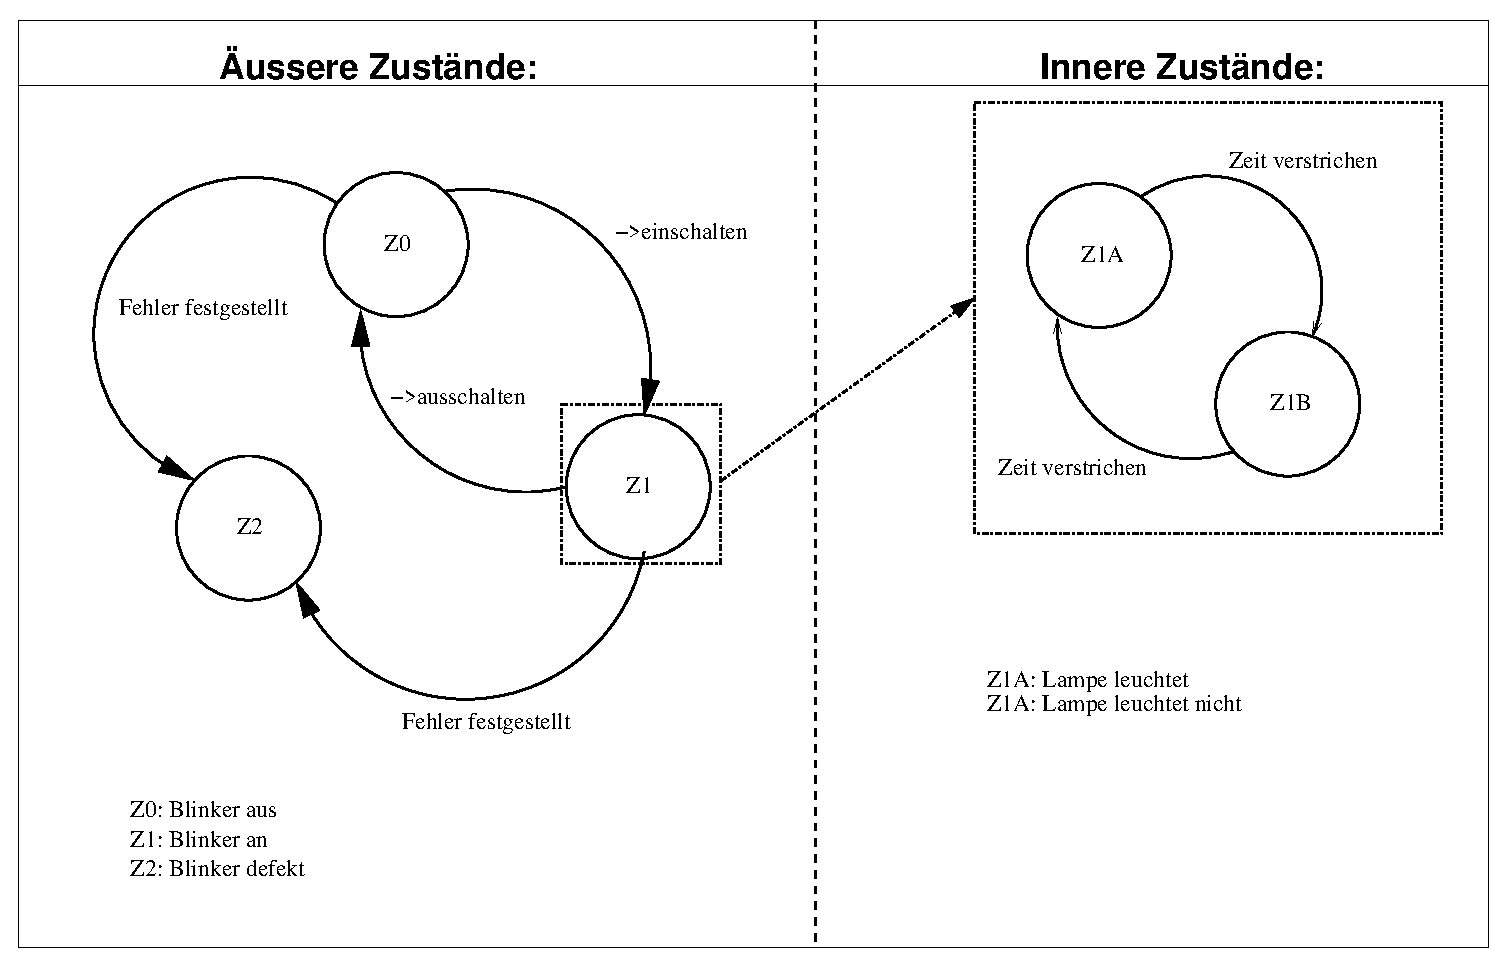
\includegraphics[width=14cm]{mw/bilder/zustaende.eps}
  \caption{�bergangsdiagramm eines modellhaften Blinkers. Fette Linien
  bedeuten �berg�nge, die vom Treiber aus ausgel�st wurden.}
  \label{mw_blinker_zustaende}
\end{figure}



Grundbausteine der Kommunikation im L�ufer sind so genannte
Nachrichten\footnote{im folgenden auch: Message}, die von einem
Bus\-teil\-nehmer zum anderen gesendet werden.  Jeder Busteilnehmer
erh�lt dazu eine im System eindeutige Nummer, die sogenannte
ID\footnote{ID: f�r IDentifier}.  �ber die Komponenten-ID wird die
Verbindung zwischen einem realen Ger�t, also z.B. einem
Scheibenwischer und dem entsprechenden Treiber auf dem PDA
hergestellt.  Die Kommunikationsstruktur des L�ufers macht das Routing
der Nachrichten �ber den CANBus f�r den Entwickler transparent, d.h.
er mu� sich lediglich darum k�mmern, da� sich sein Ger�t und der
dazugeh�rige Treiber unter der selben ID beim System anmelden.

Die eigentliche Kommunikation erfolgt dann wie schon gesagt in Form
von Nachrichten, die zwischen dem Treiber und dem zu ihm geh�renden
Ger�t ausgetauscht werden.  Bei den Nachrichten handelt es sich immer
um einen Befehl (8Bit) mit optionalen Parametern (15Bytes).  Dadurch
kann sich jeder Entwickler f�r sein Ger�t einen eigenen Satz an
Befehlen definieren, ohne da� der Befehlsatz jedes Ger�tes den anderen
Teilnehmern im System bekannt sein mu�.  Details zur Kommunikation
finden sich in Kapitel \ref{jameson_kapitel}.



\subsection{Implementierung}\label{mw_klasse}
Ziel der Entwicklung der Klassenbibliothek ist es, die Entwicklung
darauf aufsetzender Komponenten so einfach wie m�glich zu machen, da
die Entwickler, die die Komponenten entwickeln werden, sich neben der
Programmierung auch noch anderen Teilen ihrer Komponente widmen
m�ssen.  Die auf der entwickelten Bibliothek aufsetzenden Module sind
genauer:

\begin{description}
\item[Treiber] Die Treiber stellen ein Interface zu den einzelnen
  mechatronischen Komponenten her.  Dazu sollen sie das Ger�t durch
  eine Klasse repr�sentieren, die als Methoden die speziellen
  F�higkeiten des Ger�tes exportiert.  Hierzu ist es n�tig, den
  Entwicklern durch die Klassenbibliothek ein Interface zum CANBus
  zur Verf�gung zu stellen.  Au�erdem m�ssen die Treiber auf
  Nachrichten sowohl von der GUI als auch von ihrem Ger�t am CANBus
  reagieren k�nnen.
  
\item[GUI] Die GUI soll sp�ter das Interface zum Fahrer darstellen.
  In ihr werden alle F�den zusammengef�hrt werden, die als Methoden
  aus den einzelnen Klassen laufen.  Dazu mu� es f�r den Entwickler
  der GUI einfach sein, auf die Methoden der Treiber zuzugreifen und
  deren Statusmeldungen zu erhalten.

\end{description}

Die genannten Module sind nicht Teil der vorliegenden Studienarbeit,
da ihre Implementierung im Falle der Treiber am besten durch den
Entwickler der mechatronischen Komponenten durchgef�hrt wird.  Nur der
Entwickler hat das Detailwissen, um die Treiber dem mechatronischen
Ger�t angemessen zu entwickeln.  Im Falle der GUI kann diese erst dann
erstellt werden, wenn alle Fahrzeugkomponenten feststehen, da in ihr
auch die Fahrzeuglogik festgehalten wird. Um die Fahrzeuglogik zu
implementieren, bedarf es genauerer Kenntnisse der Fahrdynamik des
L�ufers als die Autoren haben k�nnen, schon aufgrund ihrer
Fachrichtung.

Aufgabe ist es also, zwei Schnittstellen zu definieren. Im einzelnen
sind es die Anbindung der GUI an die Treiber sowie die Kommunikation
zwischen Treiber und CANBus.

\subsection{Anbindung der GUI an die Treiber}
Die GUI mu� Befehle an die Treiber geben k�nnen.  Das l��t sich recht
einfach dadurch erreichen, da� die Treiber als lokale Variablen in der
GUI Vorliegen.  Die GUI wird also zum Hauptbestandteil des
Software-Systems des L�ufers.

Die umgekehrte Kommunikation gestaltet sich etwas schwieriger.  Bei
der Anbindung der GUI an die Treiber kann man grunds�tzlich
Verschiedene Wege gehen:
\begin{description}
\item[Callback] Zum einen kann man allen Treibern bei der
  Initialisierung einen Pointer auf die GUI �bergeben.  Dabei mu� aber
  jeder Treiber die GUI und ihre Methoden schon kennen.  Da diese aber
  nicht Teil der vorliegenden Arbeit sein kann, ist die verbreitete
  Methode des Callback f�r unsere Anwendung leider nicht sehr
  geeignet.
  
  Eine Alternative hierzu w�re es, dem Treiber ein vermittelndes
  Objekt zu �bergeben, das eine Methode enth�lt, die einen String
  entgegennimmt.  Hierduch kann man die gew�nschte Flexibilit�t
  erreichen, da ein sp�terer Autor der GUI mittels Stringvergleichen
  erkennen kann, was f�r ein Ereignis aufgetreten ist.
  Stringvergleiche sind allerdings nicht sehr effizient und auch im
  L�ufer gar nicht n�tig, wie im folgenden Text deutlich wird.
  
\item[Polling] Die GUI k�nnte auch die Treiber in regelm��igen
  Abst�nden Pollen, d.h. eine bestimmte im Framework zu definierende
  Methode der Treiber-Objekte aufrufen.  �ber einen solchen
  Mechanismus w�rde dann jeder Treiber Rechenzeit erhalten und k�nnte
  eingehende Nachrichten bearbeiten.
  
  Die Methode des Polling bietet die gew�nschte Flexibilit�t, da die
  GUI nur noch die Treiber kennen mu�, aber nicht umgekehrt.
  Allerdings ist es offensichtlich, da� ein solches Vorgehen starke
  Probleme hinsichtlich der Leistung hat.  Zum einen wird so keine
  bedarfsgerechte Verteilung der CPU Leistung erreicht und zum anderen
  kostet das unn�tige Aufrufen von Methoden, die derzeit nichts zu tun
  haben, unn�tig Rechenzeit.
  
\item[Signals und Slots] F�r die GUI kommt das Produkt ,,QTOPIA'' der
  Firma Trolltech zum Einsatz, folglich stand eine weitere M�glichkeit
  zur Verf�gung, die Kommunikation zwischen Treiber und GUI zu
  realisieren.  Die auf QTOPIA basierende L�sung ist im Gegensatz zu
  den anderen Ans�tzen nicht zu den Standard-Techniken zu z�hlen,
  weshalb hier eine Erl�uterung des bei Trolltech entwickelten
  Verfahrens gegeben werden soll.
  
  QT verf�gt �ber einen Mechanismus, der mit sogenannten ,,Signals''
  und ,,Slots'' arbeitet.  Signale und Slots k�nnen eine beliebige
  Anzahl Argumente beliebigen Typs �bermitteln und sind �berdies
  typsicher.
    
  Ein Objekt verschickt Signale, durch welche Slots von verkn�pften
  (connected) Objekten aufgerufen werden. Am besten l��t sich dies an
  einem kleinen Beispiel zeigen:
  
\begin{verbatim}
class Foo : public QObject
 {
  Q\_OBJECT
  public:
    Foo();
    int  value() const { return val; }
  public slots:
    void setValue( int );
  signals:
    void valueChanged( int );
  private:
    int  val;
 };
\end{verbatim}
    
  Die Ausdr�cke ,,Q\_OBJECT'', ,,slots'' und ,,signals'' werden vom
  Meta Object Compiler (moc) ben�tigt.  Dieser Compiler erzeugt ein
  neues C++-Sourcefile, das Code enth�lt, der das Objekt
  initialisiert.  Dieses File mu� compiliert und zu den anderen
  Objekt-Files gelinkt werden.  Die genannten Ausdr�cke werden vom
  Pr�prozessor entfernt bzw. so ver�ndert, da� der C++-Compiler den
  Code problemlos �bersetzen kann.
    
  Die Implementation von Foo::setValue():
\begin{verbatim}
void Foo::setValue( int v ) 
 {
   if ( v != val ) {
    val = v;
    emit valueChanged(v);
   }
 }
\end{verbatim}
  
  Ein weiterer moc-Ausdruck ist ,,emit'', womit ein Signal versendet
  wird.  Nun werden zwei Instanzen von Foo miteinander verbunden:

\begin{verbatim}
Foo a, b;
connect(&a, SIGNAL(valueChanged(int)), &b, SLOT(setValue(int)));
b.setValue( 110 );
a.setValue( 88 );
b.value();          // gibt 88 zur�ck
\end{verbatim}
    
  Durch Aufrufen von a.setValue() verschickt a ein Signal, worauf der
  damit verbundene Slot b.setValue() aufgerufen wird.
  
  Durch den Signal/Slot-Mechanismus von QT k�nnen zwei Objekte
  zusammen\-arbeiten, ohne da� sie sich gegenseitig kennen (es mu� nur
  jemand da sein, der sie verkn�pft).  Ein solcher Mechanismus
  erleichtert die Programmierung von GUIs ungemein, da in einem neuen
  Widget\footnote{Element einer graphischen Oberfl�che} oft
  Standardkomponenten wie Pushbuttons etc. eingebunden werden m�ssen.
  QT �bernimmt f�r den Programmierer die Verwaltung solcher
  Standardkomponenten, sie m�ssen nur dynamisch alloziert (mit new)
  und connected werden.
  
  Genau das ist aber auch bei der Kommunikation im L�ufer mehr als
  n�tzlich: Die Treiber k�nnen unabh�ngig von der GUI entwickelt
  werden und auch in eventuellen Nachfolgeprojekten Verwendung finden.
  Sie stellen ihre Funktionalit�t als Slot zur Verf�gung und
  emittieren Signale, wenn sie der GUI etwas mitteilen wollen.  Wohin
  die Signale dann geleitet werden, ist Sache desjenigen, der den
  Treiber verwenden wird.
  
  Die beschriebene gro�e Flexibilit�t gab den Ausschlag f�r eine
  Entscheidung zugunsten eines solchen Ansatzes.  Informationen �ber
  QT finden sich unter \cite{mwtt}.  Der einzige Nachteil der
  beschriebenen L�sung ist die Abh�ngigkeit von QT, was bei der
  Nutzung von QT als GUI f�r den PDA aber kein gro�es Hindernis
  darstellt.

\end{description}

\subsection{Zugriff der Treiber auf den CANBus}
F�r den Zugriff auf den CANBus kann man ebenfalls die sehr m�chtigen
Strukturen von QTOPIA nutzen.  In einem solchen Fall sendet das
Framework ein Signal, da� eine neue Nachricht vorliegt.  �ber einen
Verteilermechanismus w�rde die Nachricht dann als Signal an einen
Slot des entsprechenden Treibers gesendet.

Im L�ufer wird ein solcher Ansatz allerdings nicht verfolgt.  Statt dessen
erben alle Treiber von einer gemeinsamen Basisklasse, die die
Funktionalit�t des Sendens und Empfangens von Nachrichten zur
Verf�gung stellt.  Das Empfangen ist dabei eine abstrakte virtuelle
Methode, die von jedem Treiber einzeln implementiert werden mu�.
Hierzu haben die folgenden beiden �berlegungen gef�hrt:

Zum einen den Teil der Bibliothek, der nicht direkt mit der GUI
zusammenh�ngt, m�glichst portabel zu gestalten.  Das bedeutet auch,
da� man sich in diesem Bereich nicht von QT's Pr�prozessor abh�ngig
machen kann.

Zum anderen sind die anzubietenden Funktionalit�ten in dem Teil des
Frameworks wesentlich �bersichtlicher und auch schon im Laufe der
vorliegenden Arbeit bekannt: Das Senden und Empfangen von Nachrichten.
Die genaue Kenntnis der anzubietenden Funktionen nicht zu nutzen w�rde
unn�tige Komplexit�t im Programm hervorrufen und die Bibliothek nur
unn�tig vergr��ern.

\subsection{Implementierungsdetails}
%Abbildung \ref{mw_uml} zeigt ein UML der entstandenen Bibliothek.
Auf Details zur Implementierung soll an dieser Stelle unter Hinweis
auf die im Anhang vorhandene API\footnote{API: Application Programming
  Interface}-Referenz verzichtet werden.

%UPDATEN
%\begin{figure}
%  \center 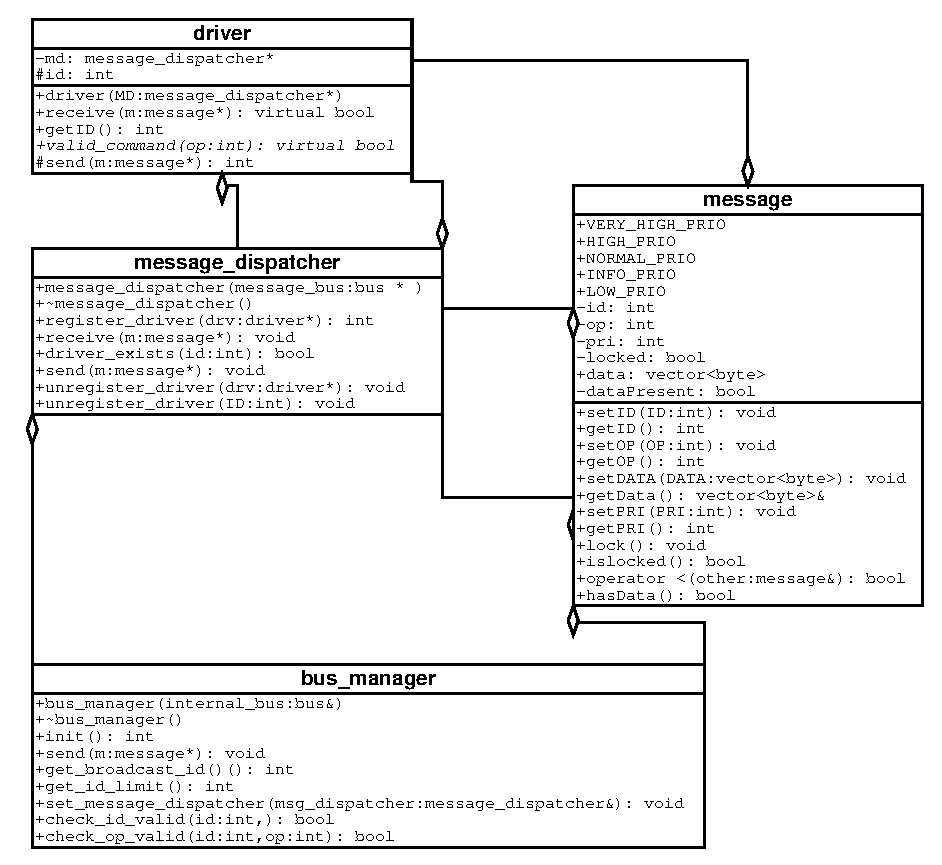
\includegraphics[width=15.0cm]{mw/bilder/uml.eps}
%  \caption{UML der Klassenbibliothek}
%  \label{mw_uml}
%\end{figure}


%------------------------------------------------------------
\newpage
\section{Entstandene Software: DebugTreiber}

\subsection{Zweck des Tools}
Im Rahmen der Gespr�che mit den ebenfalls am Projekt L�ufer
beteiligten Maschinenbau-Studenten kam immer mehr zum Vorschein, da�
f�r die Entwicklung der mechatronischen Teile noch zus�tzliche
Werkzeuge ben�tigt werden.  So ist es f�r eine z�gige Entwicklung von
Komponenten nicht vertretbar, die Hardware parallel zum Treiber
entwickeln zu m�ssen.

Ein Entwickler z.B. eines Blinkers sollte die M�glichkeit erhalten,
seine Hardware zu testen, ohne tats�chlich schon den Treiber dazu
entwickelt zu haben. Der Entwickler wei�, welche ID\footnote{Diese
  jeder Komponente eindeutig zugeordnete Nummer mu� allerdings f�r
  jedes mechatronische Gesamtsystem zentral vergeben werden, da ein
  globaler Addressraum, wie ihn z.B. Ethernet bietet, nicht zur
  verf�gung steht.}sein Ger�t hat und welche Operationen es versteht.
Folglich kann er die korrekte Funktionsweise durch manuelle Eingaben
und Beobachten der Reaktion seines Ger�tes �berpr�fen. Beobachten kann
er entweder �nderungen am Ger�t selber (z.B.: Lampe blinkt) oder aber
R�ckmeldungen des Ger�tes �ber den CAN-Bus.  Um den
Hardware-Entwicklern die Arbeit zu erleichtern, erm�glicht der
DebugTreiber nun genau das: Manuelles Senden und Empfangen von
Nachrichten an ein bzw. von einem bestimmten Ger�t.

Da wir bei der Kommunikation zwischen Ger�t und Treiber (siehe
\ref{mw_com}) ein hinreichend generisches Verfahren einsetzen, war es
leicht m�glich, ein Programm zu entwickeln, das einen solchen
,,Handbetrieb'' eines Ger�tes erm�glicht.

\subsection{Funktionalit�ts�bersicht}

\subsubsection{Senden}
Abbildung \ref{mw_screen_senden} zeigt die GUI zum Senden einer
Message an ein Ger�t am CAN-Bus.  Wie in \ref{mw_com} beschrieben setzt
sich das Protokoll aus Operationen und eventuellen Parametern
zusammen.

Die Messages kann man hier (numerisch) zusammenstellen, um dem unter
,,Setup'' eingestellten Ger�t eine Message zu senden.  Die GUI sollte
weitgehend selbsterkl�rend sein.  Sie verhindert, da� man Parameter
eingibt, die nicht gesendet werden, indem man vorher ausw�hlen mu�,
wieviele Parameter es denn werden sollen.  Einstellen kann dies ein
Benutzer mit dem Eingabefeld ,,Anzahl Datenbytes''.

Ein solches Tool kann (und will) allerdings nicht verhindern, da�
einem Ger�t Befehle gesendet werden, die es nicht verstehen kann.  Der
Entwickler kann und will das selbst �berpr�fen, um auch das Verhalten
seines Systems bei falschen Eingabedaten zu testen.

\begin{figure}
  \center 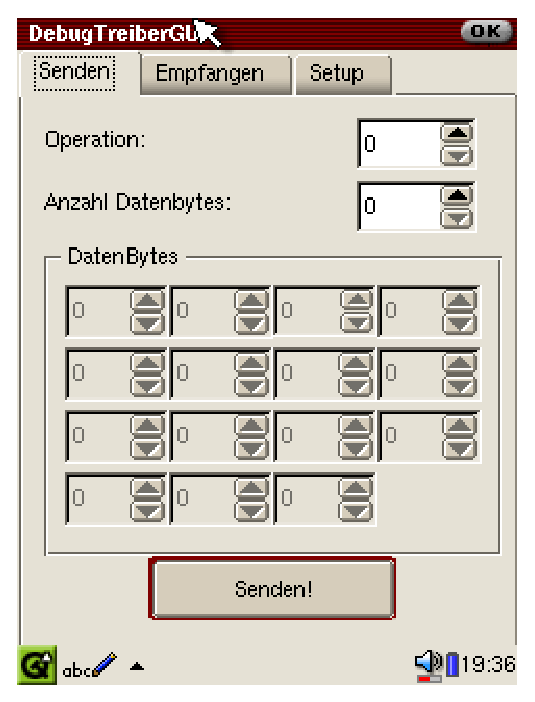
\includegraphics[width=5.0cm]{mw/bilder/GUI_senden.eps}
  \caption{Screenshot Senden}
  \label{mw_screen_senden}
\end{figure}


\subsubsection{Empfangen}
Abbildung \ref{mw_screen_empfangen} zeigt die GUI zum Empfangen von
Messages vom CAN-Bus.  Das Tool speichert eingehende Messages, die
unter der im ,,Setup'' eingestellten ID eintreffen.

Mit dem Feld ,,�bertragung'' kann man ausw�hlen, welche der
gespeicherten Messages man betrachten m�chte.  Dieses Feld zeigt
standardm��ig immer die Nummer der letzten empfangenen Message an.

Der Wechsel kann jedoch recht h�ufig sehr schnell von statten gehen.
Aus diesem Grund ist es m�glich, den Proze� zu pausieren.  Die Pause
kann der Benutzer mittels des Kontrollfeldes ,,Pause'' ausl�sen.
Einkommende Nachrichten werden bei aktivierter Pause weiterhin im
Hintergrund archiviert.

\begin{figure}
  \center 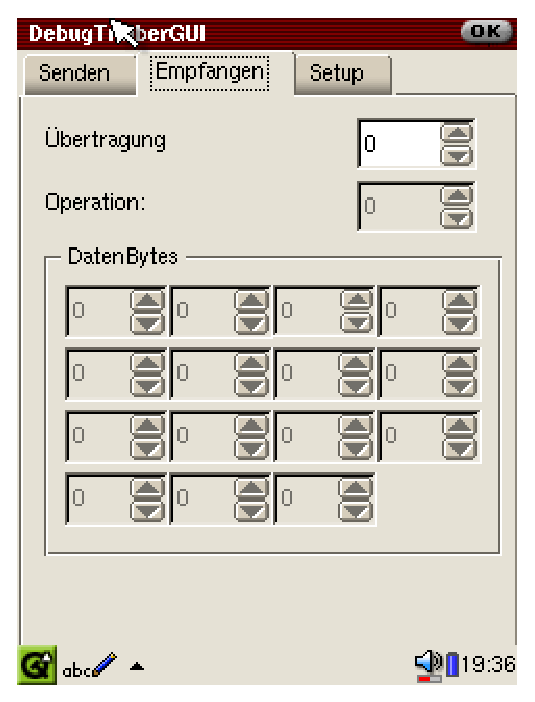
\includegraphics[width=5.0cm]{mw/bilder/GUI_empfangen.eps}
  \caption{Screenshot Empfangen}
  \label{mw_screen_empfangen}
\end{figure}

\subsubsection{Setup}
Abbildung \ref{mw_screen_setup} zeigt die GUI zum Einrichten des
Debug-Tools.  Hier kann man die gew�nschte ID des Ger�tes einstellen,
f�r das sich das Tool als Treiber registriert.  Alternativ kann man
hier ausw�hlen, einen sogenannten ,,Broadcast'' zu erstellen, der dann
an alle Busteilnehmer gesendet wird.

\begin{figure}
  \center 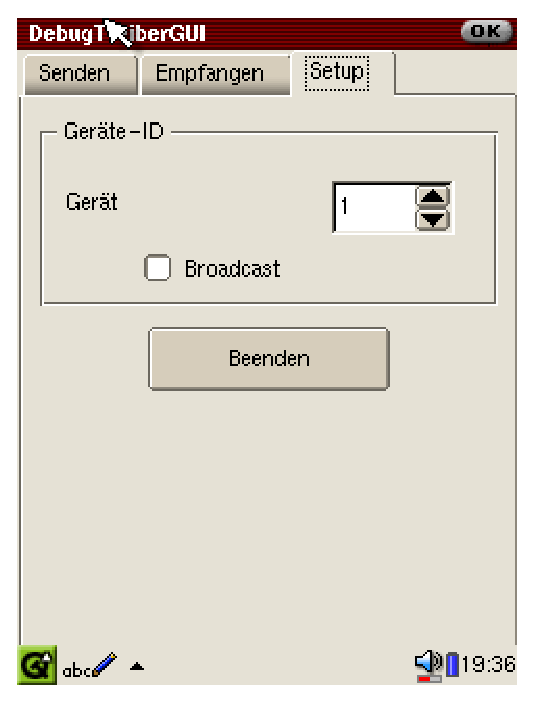
\includegraphics[width=7.0cm]{mw/bilder/GUI_setup.eps}
  \caption{Screenshot Setup}
  \label{mw_screen_setup}
\end{figure}


\newpage
\section{Fazit}
Im Rahmen dieses Teilbereichs der Mechatronik-Entwicklung f�r das
Projekt L�ufer wurde der Rahmen f�r das Fahrerinformationssystem des
L�ufers entworfen und implementiert.  Der Rahmen wird dann von den
Maschinenbauern mit ihrer spezifischen Fachkenntnis ausgef�llt
werden.

Da� das Framework hinreichend Leistungsf�hig ist, bewies die z�gige
Entwicklung der Demo f�r die Cebit 2002, bei der der L�ufer und seine
Mechatronik ausgestellt wurde.  Abbildung \ref{mw_cebit_gui} zeigt die
hierzu entwickelte GUI.  Auch bei dieser Entwicklung hat sich die Wahl
von Linux als PDA-System bew�hrt, da umfangreicher Support seitens der
Entwickler auf den entsprechenden Mailinglisten gegeben wurde, ohne
den eine solch schnelle Entwicklung sicher nicht m�glich gewesen w�re.

\begin{figure}
  \center 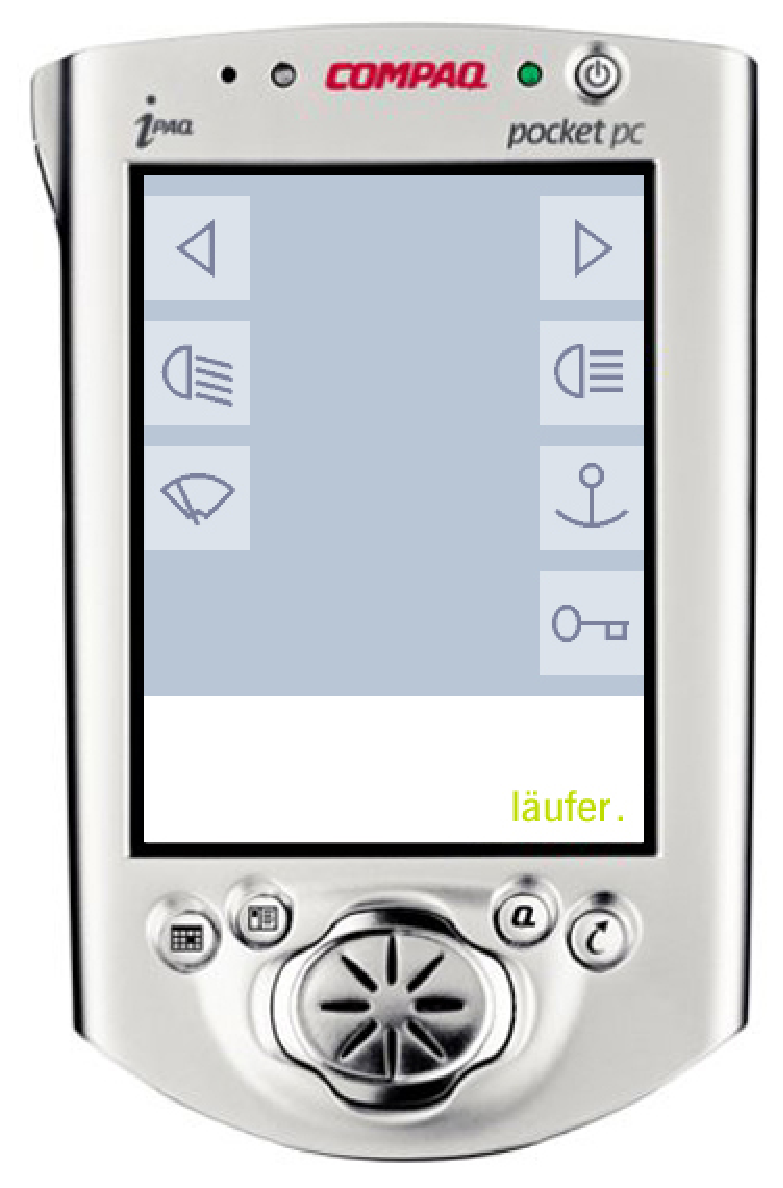
\includegraphics[width=7.0cm]{mw/bilder/Menu.eps}
  \caption{Der Compaq IPAQ mit der L�ufer-Software f�r die Cebit 2002}
  \label{mw_cebit_gui} 
\end{figure}





%%% Local Variables:
%%% mode: latex 
%%% TeX-master: "master"
%%% End:



% Jamesons Kaptitel
\chapter{Kommunikation}\label{jameson_kapitel}
von: Christoph Reichenbach
% TODO: Fazit, Einleitung

\section{Einleitung}

Der L�ufer ist kein Monolith. Nicht nur kann das wendige Fahrzeug kaum mit einem statischen Felsbrocken
verglichen werden, sondern auch-- und insbesondere-- ist sein Aufbau modular. Doch die Module schweben, wie
das im Reich der Hard- und Software nun einmal Sitte ist, nicht in isolierten Welten; Kommunikation,
Daten�bertragung zwischen ihnen ist essenziell, denn Blinker und Scheibenwischer k�nnen nicht, oder jedenfalls
bestenfalls in beschr�nktem Umfang, �ber ihre Zust�nde entscheiden, und zugleich kann und will man diese einzelnen
Elemente nicht unmittelbar mit dem Fahrer verdrahten, der bei der Fahrt meist besseres zu tun hat, als Blinker
�ber DIP-Schalter zu konfigurieren.


Dieser Abschnitt widmet der Kommunikation zwischen den Elementen des L�ufers, insbesondere zwischen der zentralen
Steuereinheit, hier durch einen PDA realisiert, und ihren Klienten. Verschiedene M�glichkeiten der Konstruktion
eines Daten�bertragungssysteme werden beschrieben und bewertet werden, mit einer abschlie�enden Beschreibung der ge-w�hlten
Kommunikationsinfrastruktur.


\section{Vor�berlegung}

Bevor wir uns in die faszinierende Welt der Daten�bertragung st�rzen, sollten wir, jedenfalls
f�r dieses spezielle Projekt, eine Grundsatzentscheidung treffen: Wollen wir ein m�glich
zentral gesteuertes Netzwerk verwenden, in dem das Maximum an Entscheidungen vom PDA
getroffen wird, oder diese Entscheidungen, soweit m�glich, den zu verwenden vorgesehenen SX-Platinen �berlassen?


Ein Vorteil einer zentralistisch angelegten Steuerung scheint, jedenfalls bei einem Reisefahrzeug,
nur schwer erkennbar; der �bliche Grund f�r solche Konstruktionen, die Minimierung von Redundanzen, greift
in einem Netz von konzeptionell ohnehin separaten Einheiten nicht. Somit sollten wir, um den
Daten�bertragungsaufwand zu minimieren, nur mehr Konfigurationsinformationen vom PDA an die Peripherie,
und umgekehrt nur wirklich auf dem PDA notwendige Informationen versenden; letztere lassen sich zusammenfassend
als f�r den Fahrer gedachte Angaben-- Geschwindigkeit, Akkumulatorstand-- und zur Weiterleitung an andere
Ger�te vorgesehene Informationen wie Zust�nde von als Peripherie angeschlossenen Lichtschaltern oder Blinker-Hebeln
beschreiben\footnote{Das Vorkommen der letztgenannten Informationen ist nicht zwingend erforderlich, falls
die Peripherie unmittelbar miteinander kommunizieren kann, z.B. durch eine Direktverbindung oder in einem
Multi-Master-Bussysstem.}.

\newpage

\section{Anforderungen an die Kommunikation}

Kommunikation, wenn nicht Selbstzweck-- wie bei allen Dingen-- mu� an der Me�latte
dessen beurteilt werden, was ihr Ziel und Zweck ist. Um von einer ``guten'' oder ``schlechten''
L�sung unsres Kommunikationsproblemes sprechen zu k�nnen, stellt sich uns somit zun�chst die Aufgabe,
die zur Bemessung der gesuchten Qualit�t dienenden Kriterien niederzuschreiben und auszuformulieren,
nicht zuletzt gegeneinander abzuw�gen, denn eine vollst�ndige Ordnung mu� sein, jedenfalls f�r ein
eindeutiges Urteil.

Das diese Abw�gung nicht einfach sein mu�, ist einleuchtend, doch f�hren wir sie trotz dieser
Vor�berlegung zun�chst aus, um eine Beurteilungsbasis zu bilden. Was also sind jene Me�latten,
die wir unsrer Kommunikationsl�sung anlegen wollen?

	\subsection{Korrektheit}

	Alle �bertragenen Daten m�ssen korrekt sein.


	Zu diesem Punkt mu� mehr gesagt werden, als sein Name hergibt. Korrektheit findet sich auf mehrere
	Arten und Weisen in unseren Forderungen wieder, die wir hier, milde axiomatisiert, auflisten wollen:

	\begin{enumerate}
	  \item{Wenn ein Datum den Empf�nger nicht erreicht, mu� der Sender davon erfahren}\label{j-correct-0}
	  \item{Wenn ein Datum den Empf�nger erreicht, mu� es zuvor versandt worden sein}\label{j-correct-1}
	  \item{Wenn ein Datum den Empf�nger mehrfach erreicht, mu� seine Semantik idempotent sein}\label{j-correct-2}
	\end{enumerate}

	Von diesen drei Forderungen ist insbesondere die Nummer \ref{j-correct-2} erl�uterungsbed�rftig. In Kommunikationssystemen
	kommt es erfahrungsgem�� vor, da� versandte Pakete aufgrund von unangemessen ausgel�sten Fehlerbehandlungen (�blicherweise,
	wenn die Best�tigung der Gegenseite einem unbemerkten �bertragunsfehler zum Opfer fiel) wiederholt versandt werden.
	Unsre obige Forderung ist nun auf zwei Weisen erf�llbar, n�mlich zum Einen, indem verhindert wird, da�
	der Empf�nger die Botschaft mehrfach erh�lt, oder zum Anderen, indem auf einer h�hergelegenen Interpretationsebene (auf die
	somit diese Fehlerbehandlung verschoben wird) der Doppelempfang ohne Folgen bleibt.

	Die erste Forderung ist in der Praxis auf eine sehr hohe Protokollebene verschiebbar, insbesondere, da wir Bidirektionalit�t fordern, ihr
	wesentlicher Vorteil, die Erkennung einer Situation, in der ein bestimmtes Ger�t vom Netz abgetrennt wurde, jedoch in
	genau dieser Situation f�r dessen bed�rfende Ger�te durch erzwungene Antworten auf alle an den Empf�nger gerichteten
	Anfragen erreicht werden kann.

	Diese drei Implikationen werden unsre Grundforderungen bilden. Da wir jedoch jenseits der Wunderbaren Welt der
	theoretischen Informatik operieren, werden sie nat�rlich nur ``in den allermeisten F�llen'' erf�llbar sein,
	aber diese Aussage bezieht sich nat�rlich auf alle unsre Forderungen. Diese speziellen Forderungen jedoch sind von der
	Art, in der sich wenig Verhandlungsspielraum-- im Gegensatz, zum Beispiel, zur �bertragungs-geschwindigkeit-- ergibt, somit
	m�ssen wir bei von uns gew�hlten Technologien stets auf ihre Erf�llung oder Erf�llbarkeit achten.

	\subsubsection{Bedeutung der Forderungen}

	Die Forderungen selbst sind �brigens durch ein triviales Modell bereits erf�llbar, einen {\it wissentlichen Nichtverschicker},
	der kein Datum versendet und den Sender davon in Kenntnis setzt (was die erste Forderung unmittelbar und die beiden anderen
	trivial erf�llt). Die Forderung, da� �berhaupt Daten �bertragen werden k�nnen, m�ssen wir somit auch ausdr�k-ken.

	%

	\subsection{Hinreichende Daten�bertragungsrate}

	Die Geschwindigkeit, mit der Daten �bertragen werden, mu� den Anforderungen des Projektes gen�gen.


	Diese Anforderung ist, in einer derartigen Formulierung, von kaum zu �bertreffender Ungenauigkeit, doch eine
	pr�zise Formulierung der be-n�tigten Daten�bertragungsrate scheint in der gegebenen Situation kaum m�glich, insbesondere,
	da die Menge der anzuschlie�enden Ger�te nicht fest gegeben ist und somit nur eine Absch�tzung gemacht werden kann,
	wieviel diese dann schlie�lich an ``laufenden'' Informationen ben�tigen beziehungsweise versenden.

	Unsre Vor�berlegung jedoch, den Ger�ten gr��tm�gliche Autonomie zu gew�hren, legt nahe, da� die Bandbreite �berschaubar
	bleiben kann; betrachten wir dazu einen typischen Extremfall:

	\subsubsection{Schnelles Tachyometer}

	Typische Geschwindigkeitsmesser in verwandten Fahrzeugen werden oft nicht h�ufiger als zwei Mal pro Sekunde mit neuen
	Informationen versorgt; ein genauer aufl�sendes Tachyometer k�nnte zum Beispiel mit der Fernseh-typischen Rate von 25 Hz eine
	als st�ndig aktuell erscheinendende Qualit�t erreichen; bei 24 Bit Datenlast (8 Bit Kennziffer, 16 Bit Information)
	w�ren dies folglich, in diesem Beispiel, 600 bps f�r dieses eine Ger�t.


	Auf die n�chsth�here glatte Zahl aufgerundet (um eventuellen Un-w�gsamkeiten, wie Datenverlust, zumindest in einem bescheidenen Ma�e
	vorzubeugen) w�ren dies 1024, f�r eine gesch�tzte Obergrenze von 16 Ger�ten also
	16384 bps im auf Datenlast eingeschr�nkten �bertragungs-verkehr-- also Kontrolldaten ignorierend-- als theoretisches Minimum.
	Das ist, aus heutiger Sicht, nicht sehr viel, was aber, nach der Vor�berlegung, unsren Erwartungen grob entspricht.


	Bandbreite alleine reicht nat�rlich nicht unbedingt; die Erz�hlung vom mit CD-ROMs beladenen G�terzug als K�nig der Bandbreite ist
	gel�ufig genug, um an eine andere h�ufige Forderung der Daten�bertragung zu erinnern.

	%

	\subsection{Geringe Latenzzeiten}

	Die Zeit, die zwischen dem Versand und dem Eintreffen eines Datenpaketes vergeht, sollte minimal sein.


	Erneut eine eher vage Forderung, die an unsere Argumentation zur nicht-Zentralisiertheit erinnert. Wie 'minimal' die Verz�gerung sein
	sollte, ist an praktischen Beispielen wohl-- abgesehen von offensichtlichen Beschr�nkungen-- am ehesten an einer doppelten
	�bertragung zwischen einem Schalter und einer anderen Peripherie, beispielsweise einem Scheinwerfer, erkennbar; hier machen sich
	hohe Latenzzeiten zwar nicht in einer gef�hrdenden, aber doch f�r den Fahrer ersichtlichen und irritierenden Weise
	bemerkbar. Bei einer nicht direkten Verdrahtung m��te also eine �bertragung zweier Botschaften innerhalb kurzer
	Zeit versandt werden k�nnen, bei
	direkter Kommunikationsm�glichkeit zwischen Schalter und Licht verringert sich dies auf eine einzelne Botschaft.

	Eine gute Latenzzeit f�r diesen Kommunikationsschritt w�re, wie im letzten Kriterium erw�hnt, 0.04s; praktisch ausreichend
	w�re jedoch auch eine schlechtere Zeit von 0.1s, da, wie erw�hnt, zu guter Letzt doch ``nur'' wieder das Empfinden des Fahrers bedient wird.

	Gerade an diesem Beispiel sieht man nat�rlich eine zuvor schon oft implizit erw�hnte notwendige Anforderung, die als n�chstes ausgef�hrt werden soll.

	%

	\subsection{Bidirektionalit�t}

	Kommunikation zwischen Peripherie und PDA sollte in beide Richtungen m�glich sein.


	Diese Forderung ergibt sich unmittelbar aus der Notwendigkeit, Informationen, wie, zum Beispiel, die aktuelle Reisegeschwindigkeit,
	aus Peripherieger�ten auszulesen.

	%

	\subsection{Unterst�tzung f�r mehr als einen Client}

	Es sollte m�glich sein, mehr als ein Peripherieger�t mit dem PDA kommunizieren zu lassen.


	�hnlich wie beim vorherigen Punkt, der Bidirektionalit�t, ergibt sich diese Notwendigkeit aus praktischen Erw�gungen. Eine
	Ermangelung an Bidirektionalit�t oder Mehr-Client-Funktionalit�t w�re zwar allgemein\\durch Verwendung mehrerer paralleler
	Kommunikationssysteme aus-\\gleichbar, eine solche Konstruktion ist aufgrund des Mehraufwandes an Hardware und der grunds�tzlich
	anderen Ansteuerung jedoch separat zu handhaben. Die angeklungene Forderung nach einem eher geringen Hard-ware-Aufwand l��t sich
	im �brigen noch verallgemeinern, wie wir im n�chsten Punkt sehen werden.
	%

	\subsection{Geringe Ressourcenanforderungen}

	Das verwendete Kommunikationssystem soll ``m�glichst wenig'' Hardware, Strom, und Prozessorleistung der beteiligten Kommunikationssysteme
	ben�tigen.



	Eine pr�zisere Angabe jenseits von offensichtlichen Schranken des\\ Machbaren sind hier nicht m�glich; dies ist ein eher komparatives Kriterium.

	%

	\subsection{Praktische Realisierbarkeit mit gegebenen Mitteln}

	Das Kommunikationssystem mu� an finanziellem und technischem Aufwand realistisch implementierbar sein.


	Insbesondere ist, rein komparativ gesehen, eine Unterst�tzung seitens der Sponsoren, sowohl materiell als auch
	mit Informationen und praktischer Unterst�tzung ein relevantes und jedenfalls im Zweifelsfall den Ausschlag gebendes Kriterium.
	%


	\subsection{Die Minimalanforderungen}\label{j-min-req}

	Um nun nicht unn�tig auszuschlie�en, wollen wir unsre Minimalforderungen derart formulieren, da� der Ausgleich fehlender
	Eigenschaften auf einer h�heren Ebene prinzipiell erlaubt sein soll, endg�ltiger Ausschlu� einer Technologie w�rde also nur
	erfolgen, wenn sie das Erf�llen eines der Kriterien (in einem angemessenen Ma�) prinzipiell ausschlie�en w�rde.

	Wir fordern von gew�hlten Technologien minimal, da� sie nicht ausschlie�en, da� folgende Kriterien erf�llt werden:
	\begin{enumerate}
	  \item{\bf Korrektheit}
	  \item{{\bf Hinreichende Daten�bertragungsrate}: Mindestens 16384 bps f�r\\ Daten alleine}
	  \item{{\bf Geringe Latenzzeit}: Maximal 0.05s pro Botschaft oder 0.1s f�r zwei Botschaften\footnote{Diese beiden Kriterien sind sehr unterschiedlich, da z.B. �ber Priorisierungsmechanismen unter Umst�nden sichergestellt werden kann, da� Botschaften, die eingingen, jedoch weiterversandt werden m�ssen, eine geringere Latenzzeit haben. Auf der anderen Seite jedoch ist es-- bei einer Latenz von konstant 0.05s-- durch zus�tzlichen Bearbeitungsaufwand m�glich, da� dennoch ein wenig mehr als 0.1s ben�tigt wird. Diese Zeit betrachten wir jedoch als unerheblich und verwenden somit 0.05s als ein einfacher zu handhabendes Kriterium.}}
	  \item{\bf Bidirektionalit�t}
	  \item{\bf Unterst�tzung f�r mindestens 16 Peripherieger�te}
	  \item{{\bf Geringe Ressourcenanforderungen}: Strombedarf auf Platine abdeckbar, eventuelle Kabel maximal handels�bliche Koaxialkabel an Dicke, 
	    sonstige Hardware sollte maximal soviel Masse haben wie der Rest der SX-Platine}
	  \item{\bf Praktische Realisierbarkeit}
	\end{enumerate}


	Mit diesen sieben Kriterien werden wir nun die verschiedenen M�glichkeiten, die sich uns zur Kommunikation bieten,
	beurteilen.

\newpage

\section{Alternativen der Kommunikationshardware}

Wir werden nun eine Reihe von Alternativen durchgehen, die uns, verbunden mit verschiedenen Vor- und Nachteilen,
Kommunikation zwischen PDA und Peripherie erlauben. Im Falle einiger dieser Technologien k�nnten die ben�tigten Anschl�sse
zwar unmittelbar auf die SX-Board aufgel�tet werden, eine Kommunikation mit dem PDA w�rde jedoch einer Zwischenstation, eines
Proxys, ben�tigen. Da auf den genannten Platinen ohnehin ein serieller Anschlu� vorhanden ist, k�nnen sie, bei
entsprechender Programmierung, unmittelbar als ein solcher dienen (sofern die verwendete Kommunikationsmethode
der Forderung nach {\bf Bidirektionalit�t} gen�gt).\\

	\subsection{Einfache Hartverdrahtung}
	
	Die einfachsten Dinge sind oft auch die besten, daher wollen wir zun�chst die Direktverbindung des PDAs mit der Peripherie �ber direkte
	Kabelverbindungen betrachten.

	Diese L�sung erf�llt zun�chst unsre Minimalanforderungen, erlaubt beliebig viele Peripherieger�te und ist an Bandbreite und Latenz nur durch
	den Systembus des SX-Controllers begrenzt. Doch schon hier stellt sich die erste Frage: Wie verbindet man die Controller direkt an ihrem
	Systembus? Ein Arbitrierungsmechanismus m��te herbei, es mu� sichergestellt werden, da� keine �bertragungen verloren
	gehen\footnote{Erste Forderung der Korrektheit}. Aber
	damit haben wir schon wesentlich mehr als eine einfache Hartverdrahtung; wenn wir jedoch unser Modell beibehalten wollen, bliebe uns nur,
	die Peripherie direkt mit den Eing�ngen der SX-Ports zu verbinden. Dies w�rde nat�rlich die Anzahl der anschlie�baren Peripherieger�te unmittelbar
	beschr�nken-- die notwendigen 16 Ger�te sollten jedoch kein prinzipielles Problem darstellen.

	Eine direkte Verbindung erzwingt jedoch einen unn�tig komplexen Kabelbaum (wenn zwei Peripherieger�te direkt
	nebeneinander liegen, ist es nicht ausreichend, sie miteinander zu verbinden-- jedes von ihnen mu� einzeln verkabelt sein). Eine derartige
	Konstruktion w�rde Masse am L�u-fer kosten und w�re fehleranf�llig; dennoch verbleibt die Hartverdrahtung als eine, wenn auch nicht
	optimale, M�glichkeit. Ihr Hauptvorteil, die hohe Geschwindigkeit und geringe Latenz (die durch zwischengeschaltete Verst�rker
	jedoch geringf�gig leiden d�rfte) ist im Projektrahmen zwar interessant, aber nicht fundamental ausschlaggebend.
	
	%

	\subsection{Drahtlose Kommunikation}

	Die Zusammenfassung aller drahtlosen Kommunikationsmittel in einer einzigen Sektion legt das Urteil �ber diese nat�rlich bereits nahe,
	daher will ich es ohne Umschweife ausformulieren.

	Drahtlose Kommunikation ben�tigt mehr Leistung als hartverdrahtete Kommunikation und ist st�rungsanf�lliger; da sie kein geschlossenes
	System erlaubt (jedenfalls nicht ohne harte Kryptographie, die jenseits der Schranken der praktischen Realisierbarkeit lag), ist
	somit auch die Erf�llung der Forderungen der Korrektheit nur schwerlich vorstellbar.
	%

%	\subsection{Universal Serial Bus (USB)}
	%
%% -- fixme -- %%

%	\subsection{IEEE 802}
	%
%% -- fixme -- %%

%	\subsection{IEEE 1394 ,,Firewire''}
	%
%% -- fixme -- %%

%	\subsection{Profibus}
	%
%% -- fixme -- %%

%	\subsection{InterBus}
	%
%% -- fixme -- %%

	\subsection{Actuator Sensor Interface (AS-i)}
	Das 1993 entworfene Actuator Sensor Interface des AS-i Konsortiums
	ist ein Master-Slave-System mit bis zu 31 Slaves, das sich insbesondere
	durch eine sehr geringe Komplexit�t auszeichnet. Tats�chlich erf�llt
	es alle Anforderungen, die von uns an ein solches Netzwerk gestellt werden;
	sein einziger wesentlicher Nachteil ist die Beschr�nkung der Gr��e des Ein- und
	Ausgangskanals auf je 4 Bit, was zu einer Verwendung von fragmentierter
	Daten�bertragung zwingt.\\
	Da wir jedoch zu sp�t von seiner Existenz erfuhren und nicht unmittelbar
	mit Unterst�tzung seitens der Sponsoren rechnen konnten, mu� seine
	Bedeutung auf eine Auff�hrung in dieser Ausarbeitung beschr�nkt bleiben.
	%
%% -- fixme -- %%

	\subsection{Controller Area Network (CAN)}

	Das Controller Area Network, 1986 von der Robert Bosch AG zur
	Multi-Master-Kommunikation im Auftrag von Mercedes entwickelt,
	erfreut sich heutzutage einer wachsenden Beliebtheit auch bei
	anderen KFZ-Her-\\stellern wie BMW, Porsche, Fiat etc., wird
	jedoch auch au�erhalb der Automobilbranche genutzt.


	Das CAN-Protokoll ist ein reines Kommunikationsprotokoll
	(welches auch vielfach bereits in Hardware implementiert
	wurde), bezieht sich also nicht auf die	verwendeten
	physikalischen Transfermedien und die dar�bergelegene
	``Objektschicht'' (wie die dar�berliegenden Schichten
	gem. OSI-Modell von der CAN-Spezifikation genannt
	werden). Zur Zeit existieren zwei relevante, im gleichen Netz
	ineroperable Protokollversionen:

	\subsubsection{CAN 1.2}
	Version 1.2 des Protokolls stellt Mechanismen zur
	Bus-Arbitrierung, Erkennung und Korrektur fehlerhafter
	Daten�bertragungen und einen vorgesehenen Adressraum von 11 Bits
	f�r angeschlossene Ger�te zur Ver-f�gung; aufgrund einer
	protokollbedingten Einschr�nkung ist jedoch ``nur''
	eine Adressierung von 2032 Busteilnehmern m�glich.\\
	Ein zur unmittelbaren Daten�bertragung verwendetes CAN-Frame
	(der Version 1.2) maximaler Gr��e beinhaltet 8 Bytes an Daten
	und belegt (inkl. Inter-frame space, dem Abstand zweier
	Frames) 111 Bit.\\
	Das Protokoll selbst l��t die genaue Hardware-Implementierung
	offen, g�ngig sind jedoch Raten von 1 Mb/s bei minimalem
	Verdrahtungsaufwand, was unsere Minimalanforderungen mehr als
	abdeckt.


	\subsubsection{CAN 2.0}
	Diese Protokollversion unterscheidet sich von CAN 1.2
	lediglich in der optionalen Verf�gbarkeit von
	29-Bit-Bezeichnern\footnote{Die Einf�hrung dieser Erweiterung
	begr�ndet sich historisch aus von der American Society of
	Automative Engineers (SAE) gestellten Anforderungen}.

	%

	\subsection{Vehicle Area Network (VAN)}

	Dieses Netzwerk, in direkter Konkurrenz zum CAN, wurde in Frankreich entwickelt, scheint sich jedoch keiner vergleichbaren
	Popularit�t zu erfreuen. Ebenfalls als Multi-Master-f�higes
	Protokoll entworfen, wurde es 1994 ISO-standardisiert, hat
	jedoch keine (uns relevant erscheinenden) markanten Vorteile
	gegen�ber seinem Konkurrenten.

	%

%	\subsection{Konklusion}

%% -- fixme -- %%
\newpage

\section{�brige Anforderungen und Umsetzung}
	\subsection{Bereits durch CAN abgedeckte Anforderungen}
	Untersuchen wir nun die gestellten Anforderungen in Bezug auf bereits
	stattgefunden habende Abdeckung durch CAN selbst:

	\begin{enumerate}
	  \item{{\bf Korrektheit}: Wir erinnern uns an die drei geforderten Eigenschaften:
	    \begin{enumerate}
	    \item{{\it Wenn ein Datum den Empf�nger nicht erreicht, mu� der Sender davon erfahren}:
	      Diese Implikation wird von CAN nicht selbst erf�llt; ein erweiterndes Protokoll m��te
	      sie sich zur Aufgabe setzen. In unmittelbarem Zusammenhang damit ergibt sich ein praktisch
	      relevantes Problem: Kurzzeitige Leitunsst�rungen k�nnen den Verlust einzelner Botschaften zur
	      Folge haben, ohne, da� die Kommunkation unbedingt zusammengebrochen w�re. Diese Situation
	      erfordert Neuversendungen der alten Daten, wird jedoch nicht von CAN abgedeckt, da dieses
	      Protokoll keine empfangenen Sendungen quittiert.
	    }
	    \item{{\it Wenn ein Datum den Empf�nger erreicht, mu� es zuvor versandt worden sein}:
	      Wird trivial von CAN erf�llt.}
	    \item{{\it Wenn ein Datum den Empf�nger mehrfach erreicht, mu� seine Semantik idempotent sein}:
	      Die Pr�misse gilt in CAN nicht, somit mu� die Konklusion nicht erf�llt werden.}
	    \end{enumerate}
	  }
	  \item{{\bf Hinreichende Transferrate}: Markt�bliche Implementierungen liefern 1 Mb/s; bei Wahl eines hinreichend
	    intelligenten Protokolles sollte die gew�nschte Mindest-Transferrate somit zu erreichen sein:
	    Eine solche Basis-�bertragungsrate liefert,
	    bei zwischen 111 ($1 \times 8$) und 440 ($8 \times 1$) Bits
	    f�r 8 Byte, also zwischen knapp 580000 und 145000 bps alleine f�r
	    Daten \footnote{falls keine Fehlerbehandlung n�tig ist}, weit mehr,
	    als gefordert.
	  }
	  \item{{\bf Geringe Latenzzeiten}:
	    Die Latenzen in CAN sind, wie allgemein in Bus-Systemen �blich, minimal. Bei 111 f�r schlechtest
	    m�gliche Frames liegt die Latenz unter 0.00012s, was dar�berliegenden Protokollen viel
	    Freiraum einr�umt.
	  }

	  \item{{\bf Bidirektionalit�t}:
	    CAN bietet, als Multi-Master-System, verschiedenste M�glichkeiten multidirektionaler Kommunikation.
	  }

	  \item{{\bf Unterst�tzung mehr als eines Clients}: Wie angedeutet, sieht CAN 1.2 eine Adressierung von bis zu 2032 Clients vor;
	    tats�chlich k�nnte durch sp�tere Auswahl auf den Empfangenen Daten diese Menge beliebig erweitert werden
	    (was im Rahmen dieses Projektes jedoch einer Begr�ndbarkeit entbehren w�rde).}

	  \item{{\bf Geringe Ressourcenanforderungen}: Die aufgef�hrten Bedingungen (Subesektion \ref{j-min-req}) werden von der handels�blichen Hardware
	    uneingeschr�nkt erf�llt.
	  }

	  \item{{\bf Praktische Realisierbarkeit}: Bei Verwendung dieser Technologie erhielten wir Unterst�tzung durch unsre
	    Sponsoren (von denen sogar eine entsprechende Empfehlung ausgesprochen worden war).
	  }
	\end{enumerate}

	\subsection{Verbleibende Anforderungen}
	Die wesentliche verbleibende Anforderung ist somit die erste Forderung der Korrektheit, die eine Notifikation
	des Senders im Falle einer fehlgeschlagenen �bertragung voraussetzt. Bevor wir uns �ber die Bedeutung dieser Forderung
	klar werden


\newpage

\section{Alternativen f�r das Kommunikationsprotokoll}

Die Wahl des Bus-Systems (f�r das wir, auf externe Empfehlung hin, CAN-Controller vom Typ
MCP2510 der Firma Microchip Technology Inc.
verwenden), war somit gefallen. Diese liefern die bereits zuvor f�r diverse Absch�tzungen verwendete �bertragungsrate
von 1 Mb/s.

%KILLME%
Offen stand jedoch noch das zu verwendende Datenprotokoll; verbreitete Protokolle sind, insbesondere in Europa,
das CANopen-Protokoll, wobei auch DeviceNet und das Smart Distributed System (SDS) sicher Optionen gewesen w�ren,
sich jedoch hierzulande durch ihre Verwendung keine unmittelbaren Vorteile ergeben h�tten. CANopen jedoch, zu dem
unter Umst�nden bereits fertige Komponenten verf�gbar gewesen w�ren, wenn auch deren Verwendbarkeit aufgrund der
besonderen Konstruktion des L�ufers zweifelhaft erscheinen w�rde, ist ein sehr komplexes Protokoll, dessen
Implementierung, gerade auch, da die sich ergebenden Vorteile in ihrem Nutzen bestenfalls beschr�nkt w�ren,
unn�tigen Aufwand ohne nennenswerten Lerneffekt verursacht h�tte.


%	\subsection{CANopen}
%% -- fixme: Mention it at the very least -- %%


%	\subsection{DeviceNet}
%% -- fixme: Mention it at the very least -- %%

%	\subsection{Smart Distributed System (SDS)}
%% -- fixme: Mention it at the very least -- %%


	\subsection{Eigenentwicklung}
%	Zuletzt blieb nun noch die M�glichkeit einer auf die Bed�rfnisse des L�ufers zugeschnittenen Eigenl�sung.
%KILLME:
	Daher schien uns die M�glichkeit einer auf die Bed�rfnisse des L�ufers zugeschnittenen Eigenl�sung als die Vielversprechendste.
%STOP KILLING ME

	Diese
	hatte zwar zun�chst den unmittelbaren Nachteil, noch nicht entworfen worden zu sein, in Anbetracht der Nicht-
	verf�gbarkeit existierender Implementierungen der andren genannten Protokolle f�r diese Plattform jedoch andererseits
	den Vorteil, mit moderaten Entwurfsaufwand den Implementierungsaufwand den Bed�rfnissen des L�ufers gegen�ber angemessen
	gestaltbar zu sein.

	\subsection{Fazit}
	Schlu�endlich fiel unsre Entscheidung schon sehr fr�h auf eine eigene Entwicklung, da der Aufwand f�r eine vollst�ndige
	Implementierung bereits existierender Protokolle (soweit ihre Spezifikationen �berhaupt �ffentlich verf�gbar waren) unseres
	Ermessens nach wesentlich h�her gewesen w�re, wohingegen die Einschr�nkung eines dieser Protokolle keine
	merklichen Vorteile gegen�ber einem solchen eignen Protokoll erwirkt h�tte. 


\newpage

\section{Das L�ufer-Protokoll f�r den CAN-Bus} 

Die Aufgaben des resultierenden Protokolls lassen sich nun wieder auf die bereits zuvor verwendeten Protokollkriterien zur�ckf�hren.
Hierbei mu� jedoch darauf geachtet werden, die Eigenheiten des CAN-Protokolls zu beachten; die Protokolle haben also nicht nur zur
Aufgabe, unsere Korrektheitsforderungen zu erf�llen, sondern auch, eine gute Anbindung an CAN zu bieten-- wobei es sich von diesem
nat�rlich aus Gr�nden eines klaren Designs zumindest in seiner Spezifikation hinreichend weit abtrennen sollte.\\

Unsere Entscheidung fiel zugunsten eines zweischichtigen Protokolldesigns, in dem eines der Protokolle die grunds�tzliche Kommunikation und das
andere einfaches Session-Management mit Timeouts spezifizierte. Die Trennung dieser beiden Dinge schien uns in Hinsicht auf die
bevorstehende Implementierung, aber auch aus Sicht der Modularit�t
sinnvoll.\\

Eine zun�chst noch offene Frage war jedoch die Form der Protokolle,
gerade auch, da CAN Unterst�tzung f�r Multi-Mastering bietet. Es wurde nun
zun�chst der Entschlu� gefa�t, das Session-Protokoll f�r eine
Master-Slave-Kommunikation auszulegen, da dies der angestrebten unmittelbaren
Kontrolle der Peripherie durch ein zentrales System entsprach; dies
erweiterten wir sp�ter um einen Notifikationsmechanismus in die andere
Richtung und bauten es somit zu einem zwei-Master-Netz aus.
Das Netzwerk-Protokoll hingegen, das auch die Aufgabe der
Adressierung bestimmter Clients �bernehmen sollte, bildete ein
Multi-Master-System mit prioritisierten Botschaften (speziell unter Ausnutzung
der Eigenschaften des CAN-Busses), aus den gleichen Gr�nden.\\

Aus theoretischer Sicht ist das Netz somit von sternf�rmiger
Topologie, die tats�chliche Verdrahtung hingegen kann nat�rlich
beliebig im Rahmen des von CAN Erm�glichten erfolgen.

	\subsection{Die beiden Protokollschichten}
	Die beiden Protokolle, mit Namen {\it LLO} und {\it LLZ} (``L�ufer Layer One'' bzw. ``Zero''), nehmen also
	zueinander signifikant andere Aufgaben wahr:

		\subsubsection{Aufgaben des LLO-Protokolls}
		Die Aufgaben des LLO-Protokolls umfassen die folgenden:
		\begin{enumerate}
		  \item{Adressierung der Klienten}
		  \item{Verpackung der zu �bertragenden Daten in Pakete des Data Link/ Network Layer (speziell CAN)}
		  \item{Busmastering}
		\end{enumerate}


		\subsubsection{Aufgaben des LLZ-Protokolls}
		Das LLZ-Protokoll �bernimmt folgende Teilaufgaben:
		\begin{enumerate}
		  \item{Session-Management}
		  \item{Erf�llung des ersten Korrektheitskriteriums}
		\end{enumerate}
		Eine ``Sitzung'' im f�r uns relevanten Sinn erstreckt sich hierbei von Aktivierung bis Deaktivierung
		des L�ufers.

		\subsubsection{Der sichere Betriebszustand}
		Beiden Protokollen ist ein Konzept zu Eigen, das den Namen ``sicherer Betriebszustand'' tr�gt, sich
		auf Klienten im Bus bezieht und
		individuell f�r jedes angeschlossene Ger�t definiert werden mu�. Dieser sichere Betriebszustand
		ist von angeschlossenen Ger�ten im Fehlerfall einzunehmen, insbesondere, wenn die Kommunikation nach
		au�en abrei�t.
\newpage

\section{Der Bezug zum OSI-Schichtenmodell}
Als kurzer Einschub soll hier noch einmal auf das OSI-Schichtenmodell
eingegangen werden, das zwar keinen leitenden Einflu� auf das Protokolldesign
hatte, wohl aber zur nachtr�glichen Klassifizierung verwendet werden kann.\\
In dem verwendeten Kommunikationssystem werden die Ebenen wie folgt belegt:

\begin{itemize}
  \item {{\bf Schicht 1: Physical Layer}: Diese Schicht findet sich in Verdrahtung, dem MCP2510, dem SX-Microcontroller, und den
    dazwischenliegenden Verbindungen.}
  \item {{\bf Schicht 2: Data Link Layer}: Die Fehlererkennung dieser Schicht ist im CAN-Protokoll spezifiziert, findet sich ent-
    sprechend physikalisch auf dem MCP2510.}
  \item {{\bf Schicht 3: Network Layer}: Ansteuerung der Komponenten wird, im Rahmen der CAN-spezifizierten Vorgaben, von einem
    von einer Implementierung des LLO-Protokolls realisiert. Die wesentliche Arbeit dabei wird durch Filtermechanismen im MCP2510
    realisiert.}
  \item {{\bf Schicht 4: Transport Layer}: Die Zerteilung in einzelne Pakete f�hrt die LLO-Implementierung durch.}
  \item {{\bf Schicht 5: Session Layer}: Die Registrierung von Busteilnehmern und Timeout-Checks bei der Kommunikation werden
    von LLZ realisiert.}
  \item {{\bf Schicht 6: Presentation Layer}: Nach- bzw. Vorbearbeitung der �bersandten Daten wird von Ger�ten und Treibern
    individuell gel�st und ist nicht Teil der hier beschriebenen Kommunikationsschicht.}
  \item {{\bf Schicht 7: Application Layer}: Die tats�chliche Durchreichung der Informationen an den Anwender, ihre optische
    Aufbereitung, automatische Beantwortung oder, allgemeiner, Versendung, findet sich in den anderen Teilen dieser Ausarbeitung
    beschrieben.}
\end{itemize}
    

\newpage

\section{Das LLO-Protokoll}\footnote{Die vollst�ndige Protokollspezifikation findet sich als Anhang (Sektion {\ref{llo-proto}}).}
Das Protokoll geht davon aus, dass versandte Daten ``ganz oder gar nicht'' ankommen, gem�� unsren Korrektheitsforderungen
(die ja zu zwei Dritteln schon von CAN erf�llt wurden). In diesem Rahmen stellt es zus�tzliche Sicherheitsmechanismen
und ein Multi-Master-Protokoll, das sich auf CAN implementieren l��t.

	\subsection{Struktur des Protokolls}

	Das LLO-Protokoll ist ein prinzipiell multi-Masterf�higes Protokoll, das die Nutzung der M�glichkeiten von Multi-Master-
	Sendungen jedoch auf asynchrone Notifikationen einschr�nkt. Somit existiert ein tats�chlicher Master in diesem Netzwerk,
	der als Controller bezeichnet wird; er erh�lt zugleich eine der 32 im Bus verf�gbaren Adressen (1) fest zugewiesen.
	Eine weitere Adresse ist f�r explizite Broadcasts (z.B. f�r eine totale Systemabschaltung im Falle der Entfernung des
	den Controller steuernden PDAs) reserviert, was 30 Adressen f�r Busteilnehmer l��t.\\
	Gerichtete und Broadcast-Adressierung sind somit m�glich; die L�nge der �bertragenen Daten ist zudem durch LLO nicht
	eingeschr�nkt.\\

	Fassen wir einmal kurz die vom Protokoll vorgesehenen Befehle mit ihren relativen Priorit�ten zusammen:
	\vspace{0.3cm}\\
	\begin{tabular}{cclp{7cm}}
	{\bf K�rzel} & {\bf Priorit�t} & {\bf Sender} & {\bf Bedeutung} \\
	\hline
	{\tt SYS} & 3 & Alle 		& Fehlermeldungen, Fehlerbehandlung \\
	{\tt ACK} & 3 & Alle 		& Best�tigung nach �bertragung \\
	{\tt KAL} & 3 & Controller 	& Keep-Alive-Signal (s. \ref{jd-llo-kal}) \\
	{\tt STX} & 2 & Controller 	& Controller $\rightarrow$ Client- Transfer \\
	{\tt RTX} & 1 & Client 		& Client $\rightarrow$ Controller- Transfer \\
	{\tt NOP} & 0 & Controller 	& Busfreigabe \\
	\end{tabular}
	\vspace{0.3cm}

	Betrachten wir nun die wesentlichen Eigenschaften des Protokolls: 

	\subsubsection{Sicherheitsmechanismen gegen Datenverlust}
	Um den Verlust von Datenpaketen wenigstens in den h�ufigsten F�llen zu bemerken, wird mit jeder �bertragung
	der Inhalt eines 4-Bit-Sequenzz�hlers versandt, der (bis auf {\tt SYS}-, {\tt KAL}- und {\tt NOP}-Nachrichten) zudem bei jeder
	nicht-Broadcast-Botschaft um eins erh�ht wird. Stellt nun der Controller oder der Client beim
	Empfang einer Botschaft ein Nicht-�bereinstimmen der Sequenznummern fest, kann er davon ausgehen, einige Botschaften verloren zu
	haben und diese neu anfordern.\\
	Diese Methode greift offensichtlich nicht immer; bei einer Datenverlustrate von $p$ ist die Wahrscheinlichkeit,
	genau 16 Nachrichten hintereinander zu verlieren, jedoch genau
	$p^{15} * (1-p)$, im Falle von Vielfachen von 16 (also allen M�glichkeiten, in denen ein Datenverlust nicht
	bemerkt w�rde) somit, f�r die Aufsummierung der Wahrscheinlichkeiten des Verlustes an der $n$ten Stelle
	$$p_n = p^{16n + 15} * (1-p)$$
	und im Limes
	\begin{equation}
	  \begin{split}
	    \lim_{n \rightarrow \inf} \sum_{k = 0}^n p_k &= (1-p) * p^{15} * \lim_{n \rightarrow \inf} \sum_{k=0}^n p^{16n}\\
	    & = (1-p) * p^{15} * \lim_{n \rightarrow \inf} \frac{p^{16(n+1)} - 1}{p^{16} - 1}\\
	    & = - \frac{(1-p) * p^{15}}{p^{16} - 1}
	  \end{split}
	\end{equation}
	Entsprechend ist bei einem ``realistischen'' Datenverlustwert die Wahrscheinlichkeit f�r einen kompletten Ausfall
	dieses Mechanismusses vernachl�ssigbar; selbst bei einem St�rfaktor von 0.1 l�ge die Wahrscheinlichkeit noch bei
	unter $10^{-15}$, sogar ein St�rfaktor von 0.9 k�nnte nur in knapp 2.6\% der F�lle einen Totalausfall dieses
	Sicherungsmechanismusses bewirken.

	\subsubsection{Keep-Alive}\label{jd-llo-kal}
	Dies alles ist im Falle einer kompletten Unterbrechung der Datenleitung jedoch wenig hilfreich. In diesem
	Fall kommt das Keepalive-Signal zum Tragen, das in regelm��igen Abst�nden vom Controller auf den Bus geschrieben wird;
	wenn nicht mindestens ein solches {\tt KAL} innerhalb von 0.3s empfangen wurde, sind Klienten dazu angehalten, sich
	selbst in den sicheren Betriebszustand zur�ckzufahren.

	\subsubsection{Busfreigabe und Client-zu-Controller-Botschaften}
	Da alle vom Controller verwendeten direkten Steuerbefehle Priorit�t �ber Client-Befehle haben (mit Ausnahme
	von {\tt ACK} und {\tt SYS}, die von Clients im Rahmen von vom Controller angesto�enen Kommunikationssequenzen
	gesandt werden d�rfen, sowie des schweren Systemfehlers {\tt SYS:EGLBL}, der alle Systeme in den sicheren Betriebszustand zwingt),
	mu� der Bus vom Controller explizit freigegeben werden. Dies erfolgt, wenn er selbst keine anstehenden Botschaften hat,
	ansonsten in regelm��igen Intervallen, mittels eines {\tt NOP}-Kommandos, das an Priorit�t geringer als das Client-nach-Controller-Kommando
	{\tt RTX} ist, das somit-- jedenfalls in der die CAN-Bus-Arbitrierung verwendenden Protokollauslegung-- dieses unterdr�ckt.\\
	{\tt RTX}- �bertragung l�uft analog zur {\tt STX}-�bertragung von Controller zu Client, verwendet jedoch einen eigenen
	Sequenzz�hler\footnote{Die historische Begr�ndung daf�r liegt im Wunsch, Vollduplex effizient unterst�tzen zu k�nnen; dies war
	relevant f�r die Verwendung von LLO �ber die serielle Schnittstelle.}.\\
	{\tt RTX}-Botschaften sind die einzigen Botschaften die, auf vier Prioritisierungsstufen, noch einmal untereinander an Wichtigkeit
	unterscheiden k�nnen. Eine genaue Spezifikation der Verwendung dieser Prioritisierung wurde im Rahmen dieser Studienarbeit nicht
	durchgef�hrt und den endg�ltig die Ger�te programmierenden Mitentwicklern �berlassen.

	\subsection{Umsetzung und Tests}
	Das LLO-Protokoll wurde in C zu Testzwecken, aber auch zur seriellen Kommunikation implementiert.
	Die Implementierung auf dem SX-Chip ist zur Zeit noch nicht abgeschlossen.

	\subsection{Einsatz im Proxy}
	Zur Kommunikation zwischen PDA und dem Rest des Busses mu� ein ``Proxy'' verwendet werden, eine
	dedizierte Platine, die der Vermittlung zwischen CAN-Bus und der seriellen Schnittstelle des PDAs dient.
	Die Kommunikation zwischen Proxy und PDA findet �ber die serielle Schnittstelle statt, die beide
	Ger�te optional auf Vollduplex betreiben k�nnen.\\
	Der Proxy selbst nimmt im Netz noch eine weitere Aufgabe wahr: Er �berpr�ft das Vorhandensein des PDAs
	und sendet einen Broadcast der Form {\tt SYS:EGLBL} im Falle des Ausbleibens von Antworten des PDAs
	(Systemabsturz, Ausfall, oder Entfernung des Ger�tes), um im Falle der Ausschaltung der zentralen
	Kontrollinstanz die angeschlossene Peripherie in den sicheren Betriebszustand zu zwingen.
\newpage

\section{Das LLZ-Protokoll}\footnote{Die vollst�ndige Protokollspezifikation findet sich als Anhang (Sektion \ref{llz-proto}).}

Das LLZ-Protokoll ist ein zustandsbasiertes Protokoll, das eine feste Maximall�nge von Botschaften vorsieht (16 Bytes, mit einer Minimall�nge von einem Byte) und
eine sehr spezifische Semantik erzwingt. Zudem implementiert es den letzten noch fehlenden Aspekt des Korrektheitskriteriums.

	\subsection{Struktur des Protokolls}

	LLZ definiert Kommunikation zwischen genau zwei Teilnehmern, von denen einer dedizierter Sender und der andere Empf�nger ist.
	Beide k�nnen Kommunikation initiieren, aber nur der Sender kann eine Antwort ``erzwingen'' lassen; zudem
	ist er auch derjenige, der den Zustand des\\ Empf�ngers kontrolliert.\\
	Das LLZ-Protokoll wird in mehreren Instanzen verwendet, wobei maximal eine pro Kanal des unterliegenden Protokolles angeboten wird
	(bei LLO werden aufgrund der maximal 30 verwendeten nicht-Controller-\newline Adressen also h�chstens 30 Instanzen des Protokolls zugleich ausgef�hrt).

	\subsubsection{Zust�nde der LLZ-Empf�nger}

	Bevor es jedoch zu einer Ausf�hrung der Daten�bertragungen des Protokolles kommt findet die Initialisierung der Busteilnehmer
	statt, bei der der Sender zugleich (m�glichst vermittels der Verwendung von Broadcasts eines unterliegenden Protokolles) �berpr�ft,
	wieviele Protokollinstanzen er zu verwenden hat, auf welchen der Kan�le des unterliegenden Protokolles also Empf�nger zu erwarten sind.\\

	Clients befinden sich initial im {\tt PRE-INIT}- Zustand, der ihnen jegliche Kommunikation auf dem Bus, mit Ausnahme der Beantwortung
	von Initialisierungssignalen ({\tt INI}) verbietet. Sobald sie ein solches Signal erhalten, gehen sie kurzfristig in einen
	weiteren Zustand ({\tt INIT}), in dem sie eine �berpr�fung der Protokollversionsnummer durchf�hren und, falls kein Fehler auftrat
	(den sie an den Sender kundtun w�rden, um Sendern, die mehrere Protokollversionen unterst�tzen, eine entsprechende Suche zu erm�glichen),
	in den {\tt RUNNING}-Zustand �ber, der ihren normalen Operationsmodus darstellt. Dabei wird ein weiteres Signal an den Sender, {\tt IOK},
	versandt.\\
	Auf Befehl des Senders hin schalten sie sich (eventuell auch schon aus dem {\tt PRE-INIT}-Zustand) in den {\tt DOWN}-Modus, der
	dem sicheren Betriebszustand entspricht.

	\subsubsection{Befehlstabelle}

	Bei der Best�tigung der erfolgreichen Initialisierung vermittels des {\tt IOK}-Blockes wird eine Tabelle der von diesem
	Ger�t unterst�tzten Befehle mitverschickt; diese Tabelle ist bitweise kodiert, wobei in 16 Bytes Raum f�r 128 Befehle geschaffen wurde.
	Eine spezifische Wahl der Befehlscodes wurde im Rahmen dieser Studienarbeit nur zu Testzwecken durchgef�hrt und wird sp�teren
	Implementierern �berlassen.\\
	Der Vorteil einer derart versandten Tabelle ist eine eingeschr�nkte ``Plug-and-Play''- Nachr�stbarkeit der Peripherie.
	Treiber seitens des PDAs\footnote{welche ihre Klienten �blicherweise auf einem bestimmten Kommunikationskanal erwarten} k�n-nen mittels
	der Befehlstabelle nun unmittelbar die Verf�gbarkeit von Funktionen, die in einer echten Teilmenge der Menge der Versionen
	der Peripherie implementiert wurde, �berpr�fen, und somit ihre Handlungen oder die von ihrer API angebotene Funktionenmenge
	entsprechend ausrichten.\\
	Alle Kommunikation �ber den Bus mu� durch einen solchen Befehl gekennzeichnet sein, der Befehl darf jedoch noch bis zu 15 Bytes
	an Parametern nehmen\footnote{Dies ist ein Kompromiss an den SX, dessen Datenb�nke genau 16 Bytes in Folge fassen}.
	Es gilt eine zus�tzliche Einschr�nkung der Form von Befehlen, die durch die Art des Timeout-Trackings
	bedingt wird: F�r alle Befehle $b$ gilt: F�r alle Parameterkonfigurationen $p, p^\prime$ gilt, da� der gesamte Zustand des Clients
	unmittelbar nach Ausf�hrung von $b$ mit $p$, ohne, da� zuvor $b$ mit $p^\prime$ ausgef�hrt wurde, identisch zum Zustand des
	Clients nach der Ausf�hrung von $b$ mit $p^\prime$ gefolgt von $b$ mit $p$ ist.\\
	Das hei�t, vereinfacht ausgedr�ckt, da� die Semantik eines Befehls sich niemals auf Zust�nde beziehen darf, die der gleiche Befehl
	modifizieren kann.
	\subsubsection{Timeouts}

	Daten�bertragungen in LLZ nehmen an, da� sie vollst�ndig und hinreichend korrekt durchgef�hrt werden oder
	jedenfalls dem �bertragenden eine Nachricht zukommt, wenn bei der
	�bertragung ein nicht korrigierbarer Fehler auftrat (im LLO-Protokoll ist das bei massivsten Datenverlusten
	und fehlschlagender Fehlerbehandlung der Fall). Von der korrekten �berpr�fung der Beantwortung von Botschaften
	geht es jedoch nicht aus, daher wird bei jeder Versendung eines Befehls $b$ mit beliebigen Parametern zum
	Zeitpunkt $t$ ein Tupel $(b, t)$ gespeichert, wobei eine (partielle) Zuordnung $\mbox{\it sent}\ b \mapsto t$ resultiert,
	also jedem $b$ ein eindeutiges $t$ (jeweils das aktuellste Datum, da, wie gefordert, gleiche Befehle sich ``gegenseitig �berschreiben'')
	zugeordnet ist.\\
	Mit dieser Information wird nun in regelm��igen Intervallen nach Timeouts von Antworten gesucht und somit der Rest des Korrektheitskriteriums
	erf�llt\footnote{Tats�chlich wird nat�rlich manchmal umsonst Alarm geschlagen, da unter Umst�nden nur die Best�tigung verloren gint, aber
	dies haben wir nicht ausgeschlossen}.

	\subsection{Umsetzung und Tests}

	Die Implementierung der Timeouts beschr�nkt sich auf den PDA; auf der Ebene der SX-Controller, also der Clients,
	ist im Allgemeinen kein ausreichender Speicherplatz f�r eine Timeout-Fehlerbehandlung; Timeouts treten zudem meist in Situationen auf,
	in denen der Client vom Netz abgetrennt ist, ein Fall, der jedoch bereits durch das periodische Keepalive-Signal
	des LLO-Busses behandelt wird.\\
	Die Implementierung und Anbindung auf Hochsprachenebene wurde abgeschlossen, auf SX-Ebene ist jedoch zum Zeitpunkt des
	Schreibens nur ein Fragment der Implementierung verf�gbar.\\
	In der ersten Implementierung ist die Beschr�nkung von Befehlen zumindest SX-seitig auf solche mit bis zu 5 Bytes an Parametern
	vorgesehen; Notifikationen ({\tt NTF}) und Kommandos ohne Antworten ({\tt CMD})  werden nicht verwendet werden.

\newpage

\section{Fazit}

Im Rahmen des Projektes wurde eine f�r die Zwecke des L�ufers geeignete Kommunikationsstruktur entworfen und getestet, eine
vollst�ndige Implementierung auch auf den Mikrocontrollern war aus verschiedenen Gr�nden bis zur Fertigstellung dieser Ausfertigung
nicht mehr m�glich und mu� im Anschlu� erfolgen.

\newpage



\section{Protokoll-Layer 1: LLO-Protokoll, Version 0}
Das L�ufer Layer 1- Protokoll hat die Aufgabe, eine zielgerichtete,
sichere �bertragung von potentiell beliebigen Datenmengen in einem
Broadcast-Netzwerk mit bis zu 30 Kommunikationsteilnehmern und potentiell
begrenzter Paketgr��e durchzuf�hren. Sicher in diesem Zusammenhang bedeutet,
da� es �berpr�ft, ob ein Rezipient die f�r ihn gedachte Botschaft erhalten
hat, und, falls nicht, eine vern�nftige Anzahl von Neu�bertragungen versucht,
nach denen es den Rezipienten als vom Netz abgetrennt registriert.
Das vorliegende Netz ist dabei sternf�rmig aufgebaut.
\\
Die hier befindliche Spezifikation bezieht sich auf Version 0 des
L�ufer Layer One (LLO)-Protokolls.\\


\subsection{Kommunikation}
Das Protokoll sieht ein Multi-Master-Netzwerk als Basis vor, mit einem
Master in der Funktion des LLO-Controllers. Das Netzwerk mu� entweder
drei Klassen von Nachrichten-Priorit�ten, oder voll-Duplex-Kom-\\munikation
unterst�tzen.\\
Im Kontrast zum LLO-Controller (kurz: Controller) werden die anderen
Busteilnehmer als LLO-Clients (kurz: Clients) bezeichnet, auch, wenn diese
Bezeichnung ihre M�glichkeiten nicht voll w�rdigt.\\

In dieser Spezifikation wird Bezug auf Timeouts genommen. Diese Timeouts
werden nicht explizit spezifiziert, mit Ausnahme des Keep-Alive-Timeouts,
um Implementierern die Wahl Bus-spezifische angemessene Timeouts zu erlauben.\\


\subsubsection{Clients}
Jedem Client ist eine eindeutige Identifikationsnummer (Port) zugeordnet, die
im Addre�bereich des Protokolls liegt (0-31 in dieser Version) und nicht
0 oder 1 ist (1 ist f�r den Controller reserviert).\\
Eine Menge von Hardware ist ein Client genau dann, wenn sie sich an einem
Port P != 0 als Client im Sinne der Protokollspezifikation verh�lt.
Aus dieser Definition folgt, da� mehr als ein physikalischer Empf�nger als
Client agieren kann; die Protokollimplementierungen auf den Clients haben
in diesem Fall Vorkehrungen daf�r zu treffen, da� ihr Verhalten auch im
Fehlerfall dieser Spezifikation entspricht.\\

Jedem physikalichen Element eines Clients ist ein sicherer Betriebszustand
zugeordnet. Sobald dieses Element feststellt, da� es von den �bertragungen
des Netzes abgetrennt wurde, mu� es s�mtliche Kommunikation beenden und
den sicheren Betriebszustand einnehmen.\\
Ein Verlassen des sicheren Betriebszustandes ist nur durch Zur�cksetzen
des Ger�tes auf einer untergeordneten Ebene m�glich (z.B. Hardware-Reset).\\


\subsubsection{Controller zu Client-\"Ubertragungen}
%---------------------------------------

\paragraph{Synchrone \"Ubertragungen\\}
%------------------------------
Eine �bertragung von einem Controller zu einem Client erfolgt unangek�ndigt
mit einer Sequenz von STX-Paketen (Synchronous Transfer); aus Sicht des
Masters:

\begin{tabular}{cl}
  $\leftarrow$  & {\tt STX(id, more) size: data}\\
  $\rightarrow$	& {\tt ACK(id, more)}\\
\end{tabular}

Graphisch dargestellt:

\vspace{0.3cm}
\begin{tabular}{|c|c|c|c|}
\hline
\hline
{\tt 010IIIII } & {\tt X00MSSSS } & {\tt LLLLLLLL} & \hspace{1cm} $\cdots$ {\tt SIZE} bytes $\cdots$ \hspace{1cm} \\
\hline
\hline
\end{tabular}

\vspace{0.3cm}

\begin{tabular}{|c|c|}
\hline
\hline
	  {\tt 011IIIII }
	  &
	  {\tt X00MSSSS } \\
\hline
\hline
\end{tabular}

\vspace{0.3cm}

Wobei die Bedeutungen wie folgt sind:\vspace{0.3cm}\\

\begin{tabular}{lcp{8cm}}
{\bf Name}	& {\bf K\"urzel} & {\bf Bedeutung}\\
\hline

{\tt STX}	& {\tt 010}	& Synchronous Transfer: Operationscode\\
{\tt ACK}	& {\tt 011}	& Acknowledgement: Operationscode\\
{\tt more}	& {\tt M}	& Flag, welches indiziert, ob noch mehr Daten in diesem	Kommunikationsstrom folgen\\
{\tt size}	& {\tt L}	& Menge an folgenden Datenbytes\\
{\tt id}	& {\tt I}	& Identit\"at des Clients (Client-Kanals)\\
{\tt seqnr}	& {\tt S}	& Sequenznummer (s. \ref{j:p1:ferr})\\
{\tt reserviert}	& {\tt X}	& Reserviertes Bit\\
{\tt data}	& 	& Sequenz von {\it size} Bytes an Daten\\
\end{tabular}
\vspace{0.3cm}\\

Wenn bei einer �bertragung das {\it more}-Flag gesetzt ist, m�ssen die
Daten der n�chstes �bertragung ans Ende der vorherigen �bertragung
angeh�ngt werden.\\
Zwischen Controller und Client findet maximal eine �bertragung
gleichzeitig statt; somit ist gew�hrleistet, da� Pakete einer �bertragung
eindeutig zugeordnet werden k�nnen.\\

Ein Ausbleiben des Acknowledgements f�r eine bestimmte, imple-\\mentierungs-
abh�ngige Zeit wird als Timeout gewertet; der Sender f�hrt in diesem Fall
eine Neu�bertragung durch.\\
Nach einer angemessenen Anzahl von versuchten Neu�bertragungen wird
schliesslich eine Fehlermeldung an die aussendende Stelle ausgegeben oder
(falls keine solche Stelle existiert) intern behandelt werden.\\

\paragraph{Broadcast-�bertragung\\}
%----------------------------

Broadcast-�bertratungen entsprechen �bertragungen, bei denen die
Zieladdresse gleich 0 ist.



\subsubsection{Client zu Controller- �betragungen}
%---------------------------------------
Diese �bertragungen sind synchron und werden mit der {\tt RTX}-Operation durch-
gef�hrt:


\begin{tabular}{cl}
$\rightarrow$ & {\tt RTX(id, more) size:data}\\
$\leftarrow$  & {\tt ACK(id, more)}\\
\end {tabular}

Die �betragungen finden statt, sobald der Controller explizit mit einer
NOP-Anweisung den Bus freigibt oder pausiert. In diesem Fall werden R-�bertragungen von
dem ausgewiesenen Sender akzeptiert, bis eine �bertragung nicht mehr das
'more'-Flag gesetzt hat oder ein unbehebbarer Fehler auftrat.
Jede erfolgreiche �bertragung wird mit einem {\tt ACK} best�tigt.


\subsubsection{Fehlererkennung und -behandlung}\label{j:p1:ferr}
%-----------------------------------
Das LLO-Protokoll geht von einem selbst fehlererkennenden Protokoll aus,
daher testet es nur auf Fehler, die eine Netz-Trennung zwischen Controller
und Client indizieren.


\paragraph{Sequenznummern\\}
Jede synchrone und asynchrone �bertragung erh�ht einen Sequenzz�hler
sowohl auf der Seite des Clients wie auch des Controllers; dieser Z�hler
hat den initialen Zustand 0 und z�hlt aufw�rts, in Schritten der Gr�sse
1, Modulo 16. Sein Zustand wird in jeder �bertragung mitgesandt und danach
erh�ht, mit der expliziten Ausnahme von {\tt SYS}-,
{\tt KAL}- und {\tt NOP}-�bertragung (bei denen er nur
mitgesandt, aber nicht erh�ht wird) sowie Broadcasts\footnote{Da die Sequenznummern von
Broadcasts nicht definierbar sind. Der Nichterfolg eines Broadcasts kann somit
nur durch Timeout der Best\"atigung erkannt werden. Dies bedeutet, dass die Empfangsreihenfolge
f\"ur Broadcasts nicht garantiert ist und reduziert deren Nutzen auf globale Fehlermeldungen.}.\\
F�r {\tt STX} und {\tt RTX} werden hierbei zwei getrennte Z�hler verwendet, um
bei gepipelinetem Versandt eine eindeutige Zuordnungsf�higkeit der Nummern
zu gew�hrleisten.


\paragraph{�bertragungen im Fehlerfall\\}
Falls bei einer �bertragung ein Fehlerfall diagnostiziert wird, wird diese
�bertragung entweder entweder erneut durchgef�hrt (wenn der Fehler vom
Sender diagnostiziert wurde), oder es wird- entweder anstelle eines {\tt ACK}
(synchron) oder statt zu schweigen (asynchron) ein {\tt SYS} zur�ckgesandt:

\begin{tabular}{cl}
  $\rightarrow$ & {\tt RTX(id, more) seq=10, size:data}\\
  $\leftarrow$  & {\tt ACK(id, more) seq=11}\\
  $\rightarrow$ & {\tt RTX(id, more) seq=14, size:data}  {\bf /* FEHLER */} \\
  $\leftarrow$  & {\tt SYS(id, more) seq=12, INVSQ}      {\bf /* Fehlersignalisierung */} \\
\end{tabular}

In diesem Fall antwortet der Sender entweder ebenfalls mit {\tt SYS} (Abbruch der
�bertragung), oder er wiederholt die �bertragung an der vom erhaltenen
{\tt SYS} indizierten Stelle. Ein Abbruch erfolgt genau dann, wenn sich die
angezeigte Sequenznummer des Empf�ngers auf eine vorhergehende Botschaft
bezieht, oder wenn die Differenz der Sequenznummern modulo 16 gr�sser
oder gleich 8 ist. Der Empf�nger synchronisiert im Abbruchsfall seine
Sequenznummer mit der des Senders.
Dieser Fehlerfall kann unter folgenden Bedingungen auftreten (unter Voraus-
setzung der Korrektheit des Controllers):
a) Ein Client verwendet eine inkorrekte Protokollimplementierung
b) Ein Client hat mehrere asynchrone Pakete verpa�t
c) Ein Client besteht aus mehreren physisch Einheiten, von denen eine echte
nichtleere Teilmenge einen Teil der �bertragungen verpa�t hat.

F�r den Fall (a) kann die Korrektheit des Empfangs im Allgemeinen nicht
gew�hrleistet werden. Fall (b) ist durch Definition der inh�renten Un-
sicherheit asynchroner Pakete abgedeckt. Kritisch ist somit Fall (c):
Die empfangenden physikalischen Einheiten m�ssen erkennen, da� eine
Geschwistereinheit einen Fehler erkannt hat, und sich ruhig verhalten.
Im Falle eines �bertragungsabbruches m�ssen auch die Einheiten, die
die Nachricht korrekt erhalten haben, die aktuelle �bertragung abbrechen,
um Konsistenz zu gew�hrleisten.

\paragraph{SYN-Request\\}
%-----------------
Ein {\tt SYN}-Request ist eine synchrone {\tt STX}-�bertragung, die eine size von 0
hat. Sie dient der Synchronisierung der Sequenznummern und ist wie eine
normale �bertragung zu behandeln, soweit das Protokoll betroffen ist.

Nach sp�testens 14 asynchronen Paketen (Broadcasts) in Folge mu� ein Sender
ein {\tt SYN}-Paket schicken, um die Synchronit�t der Sequenzz�hler zu
gew�hrleisten.


\paragraph{Systemcodes\\}
%-----------------
Bei einem SYS werden Systemcodes (meist Fehlercodes) mitversandt.
Sie sind definiert wie folgt:

\begin{tabular}{ccp{4.5cm}p{4.5cm}}
{\bf NR}& {\bf ID}	& {\bf Bedeutung}				& {\bf Kommunikation}\\
\hline
1	& {\tt EINTN}	& Interner Fehler			&Abbruch\\
2	& {\tt EINSQ}	& Unpassende Sequenznummer		&Retry oder {\tt ABORT}\\
3	& {\tt ABORT}	& �bertragung Ung�ltig, Abbruch		&Abbruch\\
4	& {\tt CONTN}	& �bertragung ab hier fortgesetzt	&Fortsetzung\\
5	& {\tt EOVFL}	& Nachricht zu lang: Buffer-�berlauf	&Abbruch\\
6	& {\tt EINVR}	& Ung�ltige Version			&Abbruch\\
7	& {\tt EGLBL}	& Globales Versagen			&Sicherer Betriebszustand\\
8	& {\tt ENRDY}	& Ger�t nicht bereit			&Retry nach Verz�gerung\\
\end{tabular}
\vspace{0.3cm}

Ein SYS:GLOBL kann als Broadcast vom Controller eingesetzt werden, um alle
Ger�te in den sicheren Betriebszustand zur�ckzufahren (und damit den Bus
effektiv zu deaktivieren).


\paragraph{Timeout\\}
%-------------
Bei synchronen Versendungen wird ggf. in einem spezifizierten Zeitraum kein {\tt ACK}
vom Empf�nger erhalten. In diesem Fall wird das Paket erneut versandt


\subsection{Keep-Alive}
%-------------

Mindestens einmal pro 100 ms mu� der Controller f�r ein Keep-Alive-Signal
({\tt KAL}) auf dem Bus sorgen. Bleibt dieses Signal f�r mehr als 300 ms aus,
so m�ssen sich alle Clients in einen sicheren Betriebszustand zur�ckfahren.


\subsection{Kodierung der �bertragungspakete}
%------------------------------------
Dieses Kapitel dokumentiert die Standardkodierung der Pakete; implementierende
Systeme k�nnen eine eigene, angemessenere Kodierung verwenden.


Graphisch pr\"asentiert sich die Kodierung wie folgt:

\vspace{0.3cm}
\begin{tabular}{|c|c|c|c|}
\hline
\hline
{\tt OOOIIIII } & {\tt XVVMSSSS } & {\tt LLLLLLLL} & \hspace{1.5cm} $\cdots$ {\tt SIZE} bytes $\cdots$ \hspace{1.5cm} \\
\hline
\hline
\end{tabular}\\
\vspace{0.3cm}


{wobei manche Befehle nur zwei Bytes verwenden und die Bedeutung der Abk\"urzungen wie folgt ist:}


\begin{tabular}{cp{10cm}}
{\bf K\"urzel} & {\bf Bedeutung}\\
\hline

{\tt O}	& Synchronous Transfer: Operationscode\\
{\tt I}	& Identit\"at des Clients (Client-Kanals)\\
{\tt X}	& Reserviertes Bit\\
{\tt V}	& Versionsnummer\\
{\tt M}	& Flag, welches indiziert, ob noch mehr Daten in diesem	Kommunikationsstrom folgen\\
{\tt S}	& Sequenznummer (s. \ref{j:p1:ferr})\\
{\tt L}	& Menge an folgenden Datenbytes\\
\end{tabular}


\subsubsection{Erstes Pr�fixbyte}
%----------------------
Das erste Byte des Paketes (Pr�fixbyte) setzt sich zusammen wie folgt:\vspace{0.3cm}\\

\begin{tabular}{ll}
{\bf Bits}	& {\bf Bedeutung} \\
\hline
7-5		& Operation \\
4-0		& Rezipient \\
\end{tabular}
\vspace{0.3cm}\\


\subsubsection{Operationen}
%------------------
\vspace{0.3cm}

\begin{tabular}{ll}
{\bf Nummer}	& {\bf ID} \\
\hline
0	& {\tt NOP}\\
1	& {\tt STX}\\
2	& {\tt RTX}\\
3	& {\tt ACK}\\
4	& {\tt SYS}\\
5	& {\tt KAL}\\
\end{tabular}


\subsubsection{Zweites Pr�fixbyte}
%-----------------------
\vspace{0.3cm}

\begin{tabular}{cl}
{\bf Bits} & {\bf Bedeutung}\\
\hline
7	& Reserviert\\
6,5	& Version (hier immer 0)\\
4	& Das 'mehr'-Flag\\
3-0	& Sequenznummer\\
\end{tabular}\vspace{0.3cm}\\


\subsubsection{STX, RTX: �betragungspakete}
%--------------------------------
In diesen Paketen folgt ein Byte mit der Anzahl der zu �bertragenden
Daten-bytes, gefolgt von entsprechend vielen Daten.


\subsubsection{ACK, NOP und KAL}
%--------------------
Diese Pakete sind nach den Pr�fixbytes leer.


\subsubsection{SYS}
%-------
Auf dieses Paket folgt genau ein Byte mit dem Identifikator der System-
Message.


\subsection{Appendix A: Implementierung auf dem CAN-Bus}
%-------------------------------------------
Bei einer Implementierung auf dem CAN-Bus (LLO/CAN) wird das komplette
erste Pr�fixbyte im Identifyer dargestellt:
\ \vspace{0.1cm}\\
\begin{tabular}{cl}
{\bf Bits}	& {\bf Bedeutung}\\
\hline
10-8	& LLO/CAN-Operation\\
7-5	& Priorit�t f�r {\tt RTX}-Botschaften, sonst 011\\
4-0	& ID des Rezipienten
\end{tabular}
\ \vspace{0.1cm}\\

\subsubsection{A.1 Codierung der LLO/CAN-Operationen}
%-------------------------------------

\begin{tabular}{cccl}
{\bf Bit 10} 	& {\bf Bit 9}	& {\bf Bit 8}	& {\bf ID}\\
\hline
0	& 0	& 0	& {\tt SYS}\\
0	& 0	& 1	& {\tt ACK}\\
0	& 1	& 0	& {\tt KAL}\\
1	& 0	& 0	& {\tt STX}\\
1	& 1	& 0	& {\tt RTX}\\
1	& 1	& 1	& {\tt NOP}\\
\end{tabular}\vspace{0.3cm}\\

Somit gilt: \{{\tt SYS}, {\tt ACK}, {\tt KAL}\} $>$ \{{\tt STX}\} $>$ \{{\tt RTX}\} $>$ \{{\tt NOP}\},
wobei A $>$ B bedeutet, da� alle Elemente von A eine h�here
Priorit�t als ein beliebiges Element aus B haben.

Bei STX und RTX wird die L�ngenangabe im daf�r von
CAN vorgesehenen Bereich gespeichert, nicht als zus�tzliches
Byte. Das Protokoll verwendet im optionalen Datenbereich also
genau ein Byte.

\label{llo-proto}

\newpage


\section{Protokoll-Layer 0: LLZ-Protokoll, Version 0}
%-------------------------------------------
Alle folgenden Aussagen beziehen sich auf Version 0 des Protokolls, mit
Ausnahme explizit gekennzeichneter Stellen.\\

Das LLZ (L�ufer Layer Zero)- Protokoll realisiert eine asynchrone
und synchrone Kommunikation �ber einen existierenden sicheren Transferkanal.
'Sicher' hat hierbei die Bedeutung, da� die erfolgreiche �bertragung
mit hoher Sicherheit ``garantiert'' wird; kommt die �bertragung nicht zustande,
tritt der Garantiefall ein und es mu� ein Fehler auf
der darunterliegenden Protokollebene ausgel�st werden.
Das Protokoll unterscheidet zwischen Empf�nger- und Senderstationen, die
verschiedene Rechte und Pflichten haben.\\
Zudem ist das Protokoll Zustandsbehaftet.\\

Im folgenden bezeichnet $\prec X$ das Ereignis, da� die Botschaft X empfangen
wurde, und $X \succ$ das vollst�ndige und erfolgreiche Versenden der Botschaft X,
ebenso wie $\rightarrow X$ (Senden) und $\leftarrow X$ (Empfangen).\\

\subsection{Kommunikation}
%----------------
Jegliche Kommunikation, mit Ausnahme einer Notifikation, wird von einem
Sender ausgel�st.\\

\subsubsection{Synchrone Kommunikation}
%---------------------------

\paragraph{Operationen und Semantik\\}
F\"ur jedes Ger\"at ist eine Menge von Operationen definiert. Diese
Operationen d\"urfen durch eine bestimmte Anzahl von Bytes parameterisiert sein.
F\"ur jede mit $\overline{x}$ parametrisierte Operation $p(\overline{x})$ gilt,
da\ss\ die Semantik des Empfangs von $p{\overline{x}^\prime}$ nach $p{\overline{x}}$
gleich der Semantik des Empfangs von $p{\overline{x}^\prime}$ ist, also, da\ss\ alle
Operationen nur Zustand {\it setzen} und {\it keine relativen Modifikationen} an ihm
durchf\"uhren.
 

\paragraph{Request\\}
%-------------
Eine synchrone Kommunikation beginnt mit einem Request, der vom Sender
ausgel�st wird. Die Notation hierf�r ist (aus Sender-Sicht)\\

\begin{tabular}{cl}
$\rightarrow$ {\tt REQ(n) <OP> [Parameter]*}\\
\end{tabular}

z.B.

\begin{tabular}{cl}
$\rightarrow$ {\tt REQ(2) SET-STATE 7}\\
\end{tabular}

(n ist 1 plus die Anzahl der Parameter). Die Operation ist ein 7-Bit-Wert
(das MSB ist reserviert); die Anzahl der Parameter ist beschr�nkt auf 15.
Auf einen Request mu� ein Response folgen. Protokollimplementierungen
m�ssen also eventuell vorher eingehende Notifikationen zur�ckstellen.\\

\paragraph{Response\\}
%--------------
Aus Sender-Sicht ist die Notation hierf�r wie folgt:

\begin{tabular}{cl}
$\leftarrow$ & {\tt RES(n) <OP> [Value]*}\\
\end{tabular}

Wobei {\tt <OP>} eine Wiederholung des Operationscodes aus dem Request ist.

\paragraph{Kommando\\}
%--------------
Statt einem Request kann auch ein Kommando ({\tt CMD} statt {\tt REQ}) abgesetzt werden.
Der einzige Unterschied ist, da� keine Response hierauf generiert wird.


\subsubsection{Asynchrone Notifikation}
%---------------------------
Der Empf�nger kann asynchron Notifikationen absetzen. Diese Notifikationen
sind wie Responses aufgebaut, haben als Transmissionsoperation (s. 1.3) jedoch
{\tt NTF} statt {\tt RES}. Insbesondere beinhalten sie auch eine Operation.
Notifikationen d�rfen nur bei au�ergew�nlichen Situationen verwendet werden.
Es bleibt Senderimplementierungen vorbehalten, Empf�nger, die Notifikationen
unangemessen mi�brauchen, per {\tt SDN} zu deaktivieren.

Jeder Einheit ist jedoch eine Notifikation pro Sekunde zuzugestehen.


\subsubsection{Spezifikation der Transmissionspakete}
%-----------------------------------------
Alle �bertragungen sind Byte-basiert. Ein Transmissionspaket mit einem
Payload der L�nge n+1 sieht aus wie folgt:

\begin{tabular}{|c|c|c|c|c|}
	prfx & dat0 & dat1 & . . .  & datn\\
\end{tabular}

I.e. ein 8-Bit-Pr�fix, gefolgt von n+1 Datenbytes.

Der Pr�fix hat folgende Form:
\vspace{0.3cm}\\
\begin{tabular}{cp{1.0 cm}p{10 cm}}
{\bf Bit}	& {\bf ID}	& {\bf Bedeutung}\\
\hline
7-5	& {\tt TOP}	& Transmissionsoperation (siehe \ref{j-app-1.3.1})\\
4	& --	& reserviert (mu� 0 sein)\\
3-0	& {\tt LEN/ ERC/ VNR}
		& {\tt LEN}: Anzahl der folgenden Bytes an Daten minus 1.
		  Falls {\tt TOP} den Wert {\tt ERR} hat, ist dies der Error-
		  code; es folgen keine weiteren Daten.
		  Falls {\tt TOP} den Wert {\tt INI} oder {\tt IOK} hat, ist hier
		  die Versionsnummer des Protokolls codiert.\\
\end{tabular}


\subsubsection{Transmissionsoperationen}\label{j-app-1.3.1}
%------------------------------
\ \vspace{0.3cm}\\

\begin{tabular}{clp{10cm}}
{\bf Code}	& {\bf ID}	& {\bf Semantik}\\
\hline
0	& {\tt SDN}	& Der Empf�nger soll einen sicheren Betriebs-
		Zustand einnehmen und s�mtliche Kommunikation
		unterbinden (siehe Sektion \ref{j-app-3})\\

1	& {\tt IOK}	& Initialisierungsantwort (Protokollversion in VNR)\\

2	& {\tt REQ}	& Sender-Operation: Synchrone Anfrage\\

3	& {\tt RES}	& Empf�nger-Operation: Synchrone Antwort\\

4	& {\tt CMD}	& Sender-Operation: Asynchrones Kommando\\

5	& {\tt NTF}	& Empf�nger-Operation: Asynchrone Notifikation\\

6	& {\tt INI}	& Initialisierungsoperation, siehe Sektion \ref{j-app-3}\\

7	& {\tt ERR}	& Protokollfehler, siehe \ref{j-app-1.3.2}\\
\end{tabular}


\paragraph{Protokollfehler\\}\label{j-app-1.3.2}
%---------------------
Falls ein Sender eine ung�ltige �bertragung absetzt, mu� der Empf�nger
ihn dar�ber benachrichtigen. Zu diesem Zweck ist {\tt TOP ERR} definiert. 

Die folgenden Werte f�r {\tt ERC} sind definiert:
\ \vspace{0.3cm}\\

\begin{tabular}{lp{11cm}}
{\bf \tt ERC}	& {\bf Bedeutung} \\
\hline
0	& Sonstiger Fehler (catch-all-code) \\
1	& Version nicht unterst�tzt \\
2	& Falsche Rolle: Sender versuchte, {\tt RES}, {\tt NTF} oder {\tt IOK} zu senden \\
3	& Schon initialisiert: {\tt INI} gesendet, obwohl der Empf�nger bereits initialisiert ist \\
4	& Fehler verschickt: Der Sender sandte ein {\tt ERR} zum Empf�nger \\
5	& Paket korrupt: Ein reserviertes Bit ist falsch gesetzt \\
6-15	& -- {\it reserviert} --\\
\end{tabular}
\ \vspace{0.3cm}\\

\subsection{Payload}
%----------
LLZ v0 �bertr�gt Datenpakete einer Gr��e von 1 bis 16 Bytes. Das erste
Byte, als ``Operation'' bezeichnet, mu� immer vorhanden sein. 


\subsection{Lebenslauf von Kommunikationsteilnehmern}\label{j-app-3}
%-------------------------------------------

Der Lebenslauf von Sendern wird in dieser Spezifikation nicht behandelt.
Empf�nger jedoch werden von Sendern initialisiert und, bei Bedarf, deaktiviert;
die entsprechenden Zust�nde und �berg�nge finden sich in 3.1.


\subsubsection{Empf�nger}
%--------------
Das LLZ-Protokoll definiert folgende Zust�nde eines Empf�ngers:
\ \vspace{0.3cm}\\

\begin{tabular}{ccp{8cm}}
{\bf Code}	& {\bf Name}		& {\bf Erkl�rung}\\
\hline
{\bf S0}	& {\tt PRE-INIT}	& Initialer Zustand. Ger�t darf keine Fehlercodes senden.\\
{\bf S1}	& {\tt INIT}		& Ger�t hat INI erhalten, noch nicht beantwortet\\
{\bf S2}	& {\tt RUNNING}		& Ger�t hat IOK geantwortet und ist im normalen	Betriebszustand\\
{\bf S3}	& {\tt DOWN}		& Ger�t hat SDN erhalten und den sicheren
                                          Betriebszustand eingenommen, es darf keine Fehlercodes mehr senden. \\
\end{tabular}
\ \vspace{0.3cm}\\


%Das Zustands�bergangsdiagramm ist wie folgt:
%
%		<SDN
%	+---------------------------+
%	|			    |
%	|   <INI     IOK>     <SDN  V
%	S0 -$\rightarrow$ S1 -$\rightarrow$ S2 -$\rightarrow$ S3
%        ^	 |
%	|	 |ERR>
%	+--------+


In Zusatenden {\bf S0}, {\bf S1} und {\bf S3} werden alle Messages ignoriert, die nicht
zu einem Zustands�bergang f�hren.


\subsubsection{Shutdown}
%------------
Beim Erreichen des {\tt DOWN}-Zustandes sollte das Kommunikationsprotokoll, soweit
m�glich, das zugrundeliegende System informieren, so da� dies einen
gesicherten "Failsafe"-Betriebszustand einnehmen kann.


\subsubsection{Initialisierung des Empf�ngers}
%-----------------------------------
Die korrekte Sequenz zur Initialisierung eines Empf�ngers verl�uft aus
Sicht des SENDERS wie folgt:

\begin{tabular}{cl}
$\leftarrow$	&{\tt INI(VNR=0)}\\
$\rightarrow$	&{\tt IOK(VNR=0) ops[16]}\\
\end{tabular}

Folgt keine Antwort, so mu� der Sender annehmen, da� der Empf�nger nicht
existiert.

Statt IOK kann auch {\tt ERR(1)} (Version nicht Unterst�tzt) gesendet werden,
siehe \ref{j-app-3.3.1}.

Das Datenfeld ops[16] beinhaltet eine Liste aller vom Ger�t unterst�tzten
Operationen, codiert in 128 Bits. Der Test auf Vorhandensein der Operation
x (f�r x $>$ 7) ist also in Hochsprachensemantik wie folgt:
\ \vspace{0.2cm}\\
{\tt have-op(x) := ((x >> 3) < n) {\bf /* Byte is defined */}\\
\mbox{\hspace{2cm}\&\& (ops[x >> 3] \& (1 << (x \& 7)))}}
\ \vspace{0.2cm}\\
Dies erlaubt die Deklaration der Operationen 0-127. Die Deklaration dient
Debugzwecken und ist in dieser Protokollversion nicht verbindlich.

\paragraph{Versionsunterschiede\\}\label{j-app-3.3.1}
%--------------------------
Falls die Protokollversion des Senders vom Empf�nger nicht unterst�tzt
wird, mu� er mit {\tt ERR(1)} antworten. Der
Sender kann dann andere Protokollversionen durchprobieren, oder mit {\tt SDN} das System deaktivieren.
\label{llz-proto}

Christians Kapitel
\chapter{Implementierung der Embedded Platinen}\label{cr_kapitel}
von: Christian R�diger
\section{Anforderungen an die Peripherieelektronik}
\subsection{Gesamtkonzept}
Die Mechatronik im Projekt L"aufer mu� einer Reihe projektspezifischer Anforderungen standhalten. Was bedeuten also die eingangs geschilderten
Zielsetzungen f�r die Peripherieelektronik?

Da sich der genaue Funktionsumfang aller mechatronischen Komponenten f"ur die Zukunft nicht absch�tzen l"asst, und neue Komponenten jederzeit einfach
einzugliedern sein sollen muss das System leicht erweiterbar sein. F�r die  Zielgruppe zur Nutzung der Platinen sind die Peripherieger�te des L"aufers
muss das System mit vertretbarem Aufwandt bedienbar sein. F�r den nutzenden Ingeneur muss der Effekt und nicht der Weg interessant sein.
Die begrenzten Resourcen eines autnomen Systems wie dem L"aufer erfordern au�erdem eine sparsame Nutzung von Energie.
Um die Fahrer nicht durch Fehlfunktionen oder Ausfall eines Ger�tes zu gef�hrden mu� das System betriebssicher sein. D.h. sowohl in der physikalischen
Auslegung als auch in der Implementierung m"ussen m"ogliche Extreme in der Nutzung des Fahrzeugs ber"ucksichtigt werden. Dies beinhaltet auch eine
gewisse Fehlertoleranz mittels ,,fail save Design''.
Nicht zuletzt muss die L�sung zum einen durch das vorhandene Know How im Umfeld des Projekt L"aufer umsetzbar als auch finanzierbar bzw. durch
Sponsoren erh�ltlich sein.
Bei der Zusammenstellung der Platine muss ausserdem auf Verf"ugbarkeit der Bauelemente sichergestellt sein.
Zu guter letzt muss eine Platine wenig Raum einnehmen um dem Design des Fahrzeugs gr"o�tm"oglichen freiraum zu gew"ahren.

Zusammengefasst ist das Ziel der Arbeit eine im mechatronischen Bereich vielseitig und einfach bedienbare Platine zu erstellen sowie die
Implementierung einer Grundfunktionalit�t.
Im folgenden wird die Umsetzung der Anforderungen im Detail besprochen.

\subsection{Flexibilit"at}
Der CAN-Bus macht ein einfaches Einklinken in den Bus an jeder erdenklichen Stelle m�glich. Dadurch ist das Gesamzkonzept schnell erweiterbar.
Ein neueres Ger�t erh�lt eien eindeutige Identifikationsnummer und wird dann durch den PDA erkannt und gesteuert. N�heres dazu findet sich im Protokollteil wieder.
Die Platine erm�glicht das Anschlie�en unterschiedlicher Ger�te ohne sich um Protokollfragen k�mmern zu m�ssen.
Die Wahl der Microcontrollers und der elektronischen Bausteine lassen dem Entwickler gr��tm�gliche Freiheit bei der Wahl der Funktionalit�t des
Peripherieger�tes. Das Layout der Platine erlaubt bei entsprechender Dimensionierung der Widerst�nde und Kondensatoren eine Versorgungsspannung von
5 bis 48 Volt. Ein Spannungswandler regelt dann die Spannung auf die f�r MOS-technologie �blichen 5 Volt herunter um die Bauelemente entsprechend zu
versorgen
\subsection{Kosten}
Die Platine enth�lt lediglich Standardbauelemente wie sie auch in der Automobilindustrie verwendet werden. Die Kosten einer komplett best�ckten Platine
belaufen sich auf etwa 150,- \geneuronarrow{}. das Layout erlaubt jedoch eine Teilbest�ckung die sich auf die f�r ein spezifisches Peripherieger�t notwendigen
Bauelemente beschr�nkt. Ein weitere wichtger Punkt bei der Kostenbestimmung war die verwndbarkeit und das zusammenspiel der Bauelemente in der
gew�nschten Zusammenstellung. Um gravierende Fehler auszuschlie�en und alle Vorstellungen umzusetzen begleitet die Firma Cetron gesammten Prozess der
Platinenentwicklung. Von der Idee, dem Prototypen, der Auswahl der Komponenten, des Microcontrollers, dem Layout der Platine in zwei Revisionen bis 
hin zur Suche nach Sponsoren f�r 12 4-Layer Platinen sowie bei der Best�ckung derselben stand die Firma Cetron mit Rat und Tat bei.
\subsection{Sicherheit}
Zum Schutz vor Strom und Spannungsspitzen sowie weitestgehend vor falscher Bedienung durch einen Entwickler wurde bei der Auswahl der Komponenten als
auch beim Layout auf Robustheit Wert gelegt. Die Platine sowie die Bauelemente enthalten eine Reihe von Schutzmechanismen wie Zener-dioden oder eine
,,Schmelzsicherung'' in Form einer besonders d�nnen Leiterbahn.
Der zweite wichtige Sicherheitsaspekt liegt in der Funktion eines etwaigen Ger�tes. Hierzu sind die Nutzer der Platine angehalten einen fail save
Zustand zu implementieren. Eine entsprechende Nachricht auf Protokollseite existiert bereits.
\subsection{Design}
Um sich in das Design des L�ufers zu integrieren sind sowohl die Erweiterbarkeit als auch die simple Gr�sse der Platine von Wichtigkeit.
Die Erweiterbarkeit ist bereits im Bereich Flexibilit�t beschrieben. Die Gr��e der Platine betr�gt  x * y cm hat also etw die Gr�sse einer Checkkarte.
 Abbildung!!!!! Platine Magnetkarte !!!!!!!!

\newpage
\section{Wahl der Komponenten}
\subsection{Microcontroller}

Die Wahl des Microcontrollers beruht auf der Empfehlung der Firma Cetron. Im folgenden werden im groben die Eigenschaften beschrieben. Weitere Details
stehen im Teil \ref{Konzeption} Konzeption der Implementierung.

Die Wahl des Microcontrollers fiel auf den SX52. Dieser Microcontroller der Firma Ubicom hat 16 sogenannte Codepages Flashrom a 512 12-Bit Worten f�r den 
Programmcode und 16 $\times$ 16 8-Bit Registerb�nke sowie eine Spezialbank zur Konfiguration. Das hei�t es stehen 8 Kilobyte (1 Byte = 12 Bit) f�r
Programmcode und $2^{8}$ 8-Bit Register zu Laufzeit zur Verf�gung.
Der SX52 hat 5 8-Bit Ports die sowohl als Input als auch als Output nutzbar sind. Es existiert ein Stromsparmodus (Sleep-mode) der zur Laufzeit an- und ausschltbar
ist. Der Microcontroller hat eine Interrupt-funktion die ebenfalls zur Laufzeit aktivier und deaktivierbar ist. Einer der 5 Ports kann als
Interrupt oder Weck-port konfiguriert werden.
Ein Besonderheit des SX ist ein komerziell erh�ltliches Programmierpaket, mithilfe dessen ein Programm schrittweise ausgef�hrt und sowohl auf
Bildschirm als auch am Microcontroller verfolgbar ist.
Dies macht die Programmierarbeit deutlich einfacher. Mit einer Taktfrequenz von 50 MHz ist der SX auch f�r eine 115 Baud �bertragung an der seriellen
Schnittstelle schnell genug.
\subsection{Peripherie}
Um eine flexible Nutzung der Platine zu sichern gilt es eine Vielzahl von Anschlu�m�glichkeiten zur Verf�gung zu stellen. Im folgenden werden die
genutzen Bauelemente und Funktionalit�t der Platine beschrieben.
\begin{description}
\item[Serial Peripheral Interface (SPI)]
Die gro�e Anzahl an Bauelementen macht eine sparsame Nutzung der I/O-Ports am Microprozessor n�tig.
Zu diesem Zweck sind der CAN-Bus-Chip, zwei Low-Side-Switches, ein Analog-Digital-Wandler und ein Digital-Analog-Wandler �ber ein SPI-Bus System mit
dem Microcontroller verbunden. Jeder dieser Bausteine hat einen Chipselect-Eingang der bei einer logischen Null den jeweiligen Baustein aktiviert. Der
Datentransfer geschieht dann zwischen Microcontroller und dem selektierten Baustein. 

Das jeweilige Chipselect wird �ber einen Multplexer gesetzt. Diese L�sung spart nicht nur wertvolle Pins am Port des Microcontrollers, sie garaniert
auch das keine zwei oder mehr Ger�te auf den Datentransfer reagieren.
\item[Kommunikation]
Neben dem SPI-Bus zur internen Kommunikation stehen eine serielle Schnittstelle und ein CAN-Bus f�r die externe Kommunikation zur Verf�gung. 
CAN -Jameson Fragen.
Die serielle Schnittstelle ist direkt �ber einen Wandlerbaustein (MAX202CSE) mit dem Microcontroller verbunden. Durch die Anbindung des 
RXD- (RXD = Receive Data) und CTS-Signals (CTS = Clear To Send) an den weckf�higen Port des Microcontrollers ist eine Aktivierung der Platine �ber die
serielle Schnittstelle m�glich.
\item[Digital-Analog-Wandler]
Angeschlossen an den SPI-Bus werden die Auszugebenden Spannungen mit 12 Bit codiert. So kann linear eine Spannung von 0 bis 12 Volt dargestellt werden.
Der Baustein von Linear Technologie LTC 1446 enth�lt zwei Digital-Analog-Wandler, so das insgesamt 24 Bit (2 $\times$ 12) �ber dan Bus �bertragen werden
m�ssen.

\item[Analog-Digital-Wandler]
Der LTC 1594 von Linear Tchnologie enth�lt einen 4-Kanal Multiplexer �ber den einer von vier Eing�ngen an den Analog-Digital-Wandler gef�hrt werden
k�nnen. Zur Konfigurations werden anfangs vier Bit �bertragen die zum einen als Aktivierung und zum anderen f�r die Auswahl des Multiplexereingangs.
Wenn ein Eingang ausgew�hlt ist, dann codiert der Analog-Digital-Wandler die anliegende Spannung bis maximal 12 Volt in 12 Bit. Die Abtastrate betr�gt
16,8 kHz.

�ber Jumper l�sst sich eine R�ckkopplung der Br�ckenausg�nge mit den Eing�ngen des Anlog-Digital-Wandlers herstellen. Das hei�t es existiert eine
direkte M�glichkeit zu Messung der ... ->->-> WAS eigentlich ??????

\item[Low-Side-Switch]

Siemens Smart Octal Low Side Switch TLE 6230 GP Short Circuit Protection 8 bit 4bit PWM

TLE1+2
\item[Digitale Ein- und Ausg�nge]

Digitale Ein- und Ausg�nge
\item[Br�cken]
2 x Infineon TLE 5206-2 5 Ampere H-Bridge for DC Motors up to 40 V 6 A peak

Br�cken
\item[Speicher]

RAM
\end{description}

\newpage

\section{Anforderungen an die Implementierung des Microcontrollers}

\subsection{Bedienbarkeit}

Konstanten
Speicherreservierung
Speicherplatzierung

Codeseg
Callseg
BANKseg

\subsection{Sicherheit}

muss der Ing machen

\subsection{Kommunikation}

Interrupt
Wake on ...

\subsection{Erweiterbarkeit}
Modulstruktur und Speichermanagement

\newpage
\section{Konzeption der Implementierung}
\label{Konzeption}
\subsection{Programmierumgebung}

SXprogramm
Debugm�lichkeiten

\subsection{Implemetierungen}
Im folgenden werden Beispielhaft einige Module und die Schwierigkeiten ihrer Programmierung beschrieben.
\begin{description}
\item[Serielle Schnittstelle]
interrupt
\item[PWM]
reverse iterations
\item[Speicher]
mini seriell
\item[SPI]
mux 
\item[Sensorik]
R�ckkopplung
\end{description}

\section{Beispielszenario Scheibenwischer}
\newpage
\section{Fazit}

\section{Ausblick}
Anleitung
C-Compiler
Techn Docu


% Schluss
\chapter{Fazit}\label{fazit_kapitel}
von: Markus Weimer
%\section{Zusammenfassung}
Insgesamt wurde ein Mechatronik-Framework entwickelt, das den
gestellten Anforderungen weitgehend gerecht wird. Teile des
Frameworks, wie die Platine und die darauf aufsetzende Software sind
bereits an der TU M�nchen im Einsatz, wo mechatronische Komponenten
f�r den L�ufer entwickelt werden. Andere Teile wie Kommunikation und
das Fahrerinterface k�nnen derzeit noch nicht eingesetzt werden, da
noch keine mechatronischen Komponenten zur Verf�gung stehen.  Deren
Entwicklungsende wird den Zeitraum der vorliegenden Ausarbeitung
�berschreiten.

Das Autoren-Team wird das Projekt L�ufer weiter begleiten, um auch die
Anwendung der im Rahmen dieser Arbeit erstellten Software zu
unterst�tzen.

Im Rahmen dieser Arbeit wurden allerdings nicht nur die im Hauptteil
beschriebenen Entwicklungen betrieben, sondern auch Erfahrungen in
Bereichen gesammelt, die nur einem Projekt offenstehen.  Diese sollen
im folgenden auch ihren Platz in dieser Ausarbeitung finden.

\begin{description}
\item[Gewinnung von Partnern] Das Projekt L�ufer setzt in seiner
  gesammten Entwicklung sehr stark auf die Zusammenarbeit mit externen
  Partnern aus Industrie und Forschung.  Dies stellt zum einen die
  praktische Umsetzbarkeit der angedachten und dem Partner
  vorgestellten Entwicklung sicher, erm�glicht aber andererseits auch
  die Nutzung externen Know-Hows.
  
  So reisten zwei der Autoren\footnote{Markus Weimer und Christoph
    Reichenbach} gemeinsam nach Bern, um an der dortigen FH deren
  L�sung f�r eine Mechatronik in einem muskelgetriebenen Fahrzeug
  kennenzulernen.  Aus den dortigen Gespr�chen folgten ma�gebliche
  Design-Entscheidungen f�r die Kommunikationsstruktur des L�ufers. Im
  fr�hen Stadium des Projektes reisten die selben Personen nach
  Saarbr�cken, um dort mit Spezialisten der Firma HighTec �ber die
  M�glichkeiten einer Verbindung zwischen PDA und CANBus zu sprechen.
  
  Sp�ter besuchten wiederum zwei der Verfasser dieser
  Arbeit\footnote{Markus Weimer und Christian R�diger} die Firma SHARP
  in Hamburg.  In einem Gespr�ch mit den dort f�r mobile Endger�te
  zust�ndigen Managern gelang es, SHARP als weiteren Industriepartner
  zu gewinnen. Dies war und ist f�r das Projekt als ganzes ein
  wichtiger Erfolg, da SHARP evtl. die Versorgung des Projektes mit
  PDAs f�r die Nullserie leisten wird. Bei Kosten um die
  600Euro je PDA ist dies ein nicht unerheblicher Posten
  bei der Frage, ob die Nullserie von zehn Fahrzeugen realisierbar
  ist.
  
\item[Interdisziplin�re Zusammenarbeit] Auch dies ist eine der St�rken
  des Projektes. Das Mechatronik-Team stie� als bisher letztes zum
  L�ufer-Team, in dem sich bis zu diesem Zeitpunkt haupts�chlich
  Maschinenbauer und Designer befanden.  Anders als in anderen
  Bereichen wird im Projekt die Unterschiedlichkeit nicht als
  Handicap, sondern als Chance verstanden.  Jedes Mitglied des
  Projektes kann sich der Unterst�tzung durch andere in deren
  jeweiligem Fachgebiet sicher sein.
  
  So erstellte z.B. der Designer des Projektes Farbschema und
  Layoutvorlagen f�r die CeBIT-Demo (s.u.). Andererseits erstellte
  Markus Weimer f�r die Webseite des Projektes einige interaktive
  Elemente\footnote{z.B. ein Kontakt-Formular} und gab Hinweise zur
  technischen Realisierung der Webseite.  Diese Zusammenarbeit der
  unterschiedlichen Fakult�ten hat auch im Bereich der Mechatronik
  L�sungen erm�glicht, die ohne Sie nicht denkbar gewesen w�ren.
  
\item[Messen] F�r die Industriepartner des L�ufers ist es nat�rlich
  von besonderem Interesse, sich mit dem L�ufer der interessierten
  �ffentlichkeit zu pr�sentieren.  Dies ist vor dem Hintergrund zu
  sehen, da� einiger der Partner im L�ufer mit Technologien arbeiten,
  die so noch nicht kommerziell erh�ltlich sind, oder nur einem sehr
  kleinen Kreis von Spezialisten bekannt sind.  Auf Messen k�nnen sich
  die Industriepartner mit dem L�ufer einen wahren Publikumsmagneten
  auf den Stand stellen, um an Ihm die eigene Technologie zeigen zu
  k�nnen.
  
  F�r das Projekt stellen Messen zum einen eine Herausforderung dar,
  da der L�ufer zum Beginn einer solchen in einem pr�sentablen Zustand
  sein mu�.  Zum anderen bergen die Messen aber auch sehr gro�e
  Chancen in sich, Kontakte zu weiteren interessanten Partnern aus
  Industrie, Forschung und Politik zu kn�pfen.
  
  Das Mechatronik-Team hatte zusammen mit dem Projekt L�ufer die
  Gelegenheit, sich auf der CeBIT 2002 auf dem Stand von IBM zu
  pr�sentieren.  W�hrend dieser Messe wurden erste Kontakte zu SHARP
  (s.o.) und auch zur C't (s.u.) aufgebaut. SHARP hat �berdies
  angedacht, das Projekt auf der diesj�hrigen Systems zu pr�sentieren.
  
\item[Medien] Ein Fahrzeug wie der L�ufer erregt nat�rlich ein
  gewisses Interesse der �ffentlichkeit und damit ebenfalls das der
  Medien.  Im Rahmen des Projektes sind schon einige
  Ver�ffentlichungen zustande gekommen.
  
  Das Mechatronik-Team hatte im Rahmen des Projektes ebenfalls die
  Gelegenheit, sich einem breiteren Publikum zu pr�sentieren. So z.B.
  in \cite{artikel}. Auch wurden Kontakte zum Computermagazin c't
  gekn�pft.  Ein Manuskript f�r einen Artikel wurde durch die Autoren
  dieser Arbeit ebenfalls eingereicht, allerdings bisher noch nicht
  ver�ffentlicht, da der zust�ndige Redakteur Urlaub hat.

\end{description}


Insgesamt hat das Projekt dieser Arbeit einen spannenden und
interessanten Rahmen gestellt, auch wenn es durch seinen aktiven
Charakter oftmals das Ziel dieser Arbeit neu definierte. Es bleibt zu
hoffen, das die Universit�tsausbildung in Deutschland zuk�nftig mehr
Studenten die Chance auf ein solches Umfeld bieten kann.



%\newpage
%\section{Ausblick}


\chapter{Danksagungen}\label{danke_kapitel}
Im Rahmen unserer Arbeit wurden wir durch einige Firmen und
Privatpersonen unterst�tzt, denen wir hier gerne danken m�chten:

\begin{description}

\item[SHARP Deutschland] F�r die Unterst�tzung unserer Entwicklung
  durch zwei Sharp Zaurus PDAs.
\item[CETRON] Dort besonders Andreas May f�r ein Offenes Ohr bei der
  Entwicklung der Platine und der darauf aufsetzenden Software.
\item[IBM] F�r die M�glichkeit, auf der CeBIT 2002 auszustellen sowie
  die Bereitstellung von Hardware.
\item
\end{description}

% Das Literaturverzeichnis
\bibliography{master}

\end{document}
